
% !TEX encoding = UTF-8
% !TEX TS-program = pdflatex
% !TEX root = tesi.tex
% !TEX spellcheck = it-IT

\documentclass[11pt,                    % corpo del font principale
               a4paper,                 % carta A4
               twoside,                 % impagina per fronte-retro
               openright,               % inizio capitoli a destra
               english,
               article]{book}    

%**************************************************************
% Importazione package
%************************************************************** 

\usepackage{amsmath,amssymb,amsthm}    % matematica
\newcommand{\R}{\mathbb{R}}
\usepackage[T1]{fontenc}  
\DeclareMathOperator{\sign}{sign} 
\DeclareMathOperator*{\argmin}{argmin}              % codifica dei font:
                                        % NOTA BENE! richiede una distribuzione *completa* di LaTeX

\usepackage[utf8]{inputenc}             % codifica di input; anche [latin1] va bene
                                        % NOTA BENE! va accordata con le preferenze dell'editor

\usepackage[english]{babel}    % per scrivere in italiano e in inglese;
                                        % l'ultima lingua (l'italiano) risulta predefinita

\usepackage{bookmark}                   % segnalibri

\usepackage{caption}                    % didascalie

\usepackage{chngpage,calc}              % centra il frontespizio

\usepackage{csquotes}                   % gestisce automaticamente i caratteri (")

\usepackage{emptypage}                  % pagine vuote senza testatina e piede di pagina

\usepackage{epigraph}			% per epigrafi

\usepackage{eurosym}                    % simbolo dell'euro

%\usepackage{indentfirst}               % rientra il primo paragrafo di ogni sezione

\usepackage{graphicx}                   % immagini

\usepackage{hyperref}                   % collegamenti ipertestuali

%\usepackage[binding=5mm]{layaureo}      % margini ottimizzati per l'A4; rilegatura di 5 mm

\usepackage{listings}                   % codici

\usepackage{microtype}                  % microtipografia

\usepackage{mparhack,fixltx2e,relsize}  % finezze tipografiche

\usepackage{nameref}                    % visualizza nome dei riferimenti                                      

\usepackage[font=small]{quoting}        % citazioni



\usepackage[italian]{varioref}          % riferimenti completi della pagina

\usepackage[dvipsnames]{xcolor}         % colori

\usepackage{booktabs}                   % tabelle                                       
\usepackage{tabularx}                   % tabelle di larghezza prefissata                                    
\usepackage{longtable}                  % tabelle su più pagine                                        
\usepackage{ltxtable}                   % tabelle su più pagine e adattabili in larghezza

\usepackage[toc, acronym]{glossaries}   % glossario
                                        % per includerlo nel documento bisogna:
                                        % 1. compilare una prima volta tesi.tex;
                                        % 2. eseguire: makeindex -s tesi.ist -t tesi.glg -o tesi.gls tesi.glo
                                        % 3. eseguire: makeindex -s tesi.ist -t tesi.alg -o tesi.acr tesi.acn
                                        % 4. compilare due volte tesi.tex.

\usepackage[style=numeric-comp,useprefix,hyperref,backend=bibtex]{biblatex}
                                        % eccellente pacchetto per la bibliografia; 
                                        % produce uno stile di citazione autore-anno; 
                                        % lo stile "numeric-comp" produce riferimenti numerici
                                        % per includerlo nel documento bisogna:
                                        % 1. compilare una prima volta tesi.tex;
                                        % 2. eseguire: biber tesi
                                        % 3. compilare ancora tesi.tex.
%\addbibresource{bibliografia.bib}
%**************************************************************
% file contenente le impostazioni della tesi
%**************************************************************

%**************************************************************
% Frontespizio
%**************************************************************

% Autore
\newcommand{\myName}{Michele Antonazzi}                                    
\newcommand{\myTitle}{Robust Door Detection in Autonomous Mobile Robots}

% Tipo di tesi                   
\newcommand{\myDegree}{Tesi Magistrale}

% Università             
\newcommand{\myUni}{Università Degli Studi di Milano}

% Facoltà       
\newcommand{\myFaculty}{Corso di Informatica}

% Dipartimento
\newcommand{\myDepartment}{Dipartimaneto di Informatica Giovanni degli Antoni}

% Titolo del relatore
\newcommand{\profTitle}{Prof.}
\newcommand{\correlatoreTitle}{Dott.}

% Relatore
\newcommand{\myProf}{Nicola Basilico}
\newcommand{\myCorrelatore}{Matteo Luperto}

% Luogo
\newcommand{\myLocation}{Milano}

% Anno accademico
\newcommand{\myAA}{2021-2022}

% Data discussione
\newcommand{\myTime}{December 2021}


%**************************************************************
% Impostazioni di impaginazione
% see: http://wwwcdf.pd.infn.it/AppuntiLinux/a2547.htm
%**************************************************************

\setlength{\parindent}{14pt}   % larghezza rientro della prima riga
\setlength{\parskip}{0pt}   % distanza tra i paragrafi


%**************************************************************
% Impostazioni di biblatex
%**************************************************************
\bibliography{bibliografia} % database di biblatex 

\defbibheading{bibliography} {
    \cleardoublepage
    \phantomsection 
    \addcontentsline{toc}{chapter}{\bibname}
    \chapter*{\bibname\markboth{\bibname}{\bibname}}
}

\usepackage{float} %per inserire figure in mezzo al testo

\usepackage{listings} % per inserire codice 

\setlength\bibitemsep{1.5\itemsep} % spazio tra entry

\DeclareBibliographyCategory{opere}
\DeclareBibliographyCategory{web}

\addtocategory{opere}{womak:lean-thinking}
\addtocategory{web}{site:agile-manifesto}

\defbibheading{opere}{\section*{Riferimenti bibliografici}}
\defbibheading{web}{\section*{Siti Web consultati}}


%**************************************************************
% Impostazioni di caption
%**************************************************************
\captionsetup{
    tableposition=top,
    figureposition=bottom,
    font=small,
    format=hang,
    labelfont=bf
}

%**************************************************************
% Impostazioni di glossaries
%**************************************************************

%**************************************************************
% Acronimi
%**************************************************************
\renewcommand{\acronymname}{Acronimi e abbreviazioni}

\newacronym[description={\glslink{apig}{Application Program Interface}}]
    {api}{API}{Application Program Interface}

\newacronym[description={\glslink{umlg}{Unified Modeling Language}}]
    {uml}{UML}{Unified Modeling Language}

%**************************************************************
% Glossario
%**************************************************************
%\renewcommand{\glossaryname}{Glossario}

\newglossaryentry{apig}
{
    name=\glslink{api}{API},
    text=Application Program Interface,
    sort=api,
    description={in informatica con il termine \emph{Application Programming Interface API} (ing. interfaccia di programmazione di un'applicazione) si indica ogni insieme di procedure disponibili al programmatore, di solito raggruppate a formare un set di strumenti specifici per l'espletamento di un determinato compito all'interno di un certo programma. La finalità è ottenere un'astrazione, di solito tra l'hardware e il programmatore o tra software a basso e quello ad alto livello semplificando così il lavoro di programmazione}
}

\newglossaryentry{umlg}
{
    name=\glslink{uml}{UML},
    text=UML,
    sort=uml,
    description={in ingegneria del software \emph{UML, Unified Modeling Language} (ing. linguaggio di modellazione unificato) è un linguaggio di modellazione e specifica basato sul paradigma object-oriented. L'\emph{UML} svolge un'importantissima funzione di ``lingua franca'' nella comunità della progettazione e programmazione a oggetti. Gran parte della letteratura di settore usa tale linguaggio per descrivere soluzioni analitiche e progettuali in modo sintetico e comprensibile a un vasto pubblico}
}
 % database di termini
\makeglossaries


%**************************************************************
% Impostazioni di graphicx
%**************************************************************
\graphicspath{{immagini/}} % cartella dove sono riposte le immagini


%**************************************************************
% Impostazioni di hyperref
%**************************************************************
\hypersetup{
    %hyperfootnotes=false,
    %pdfpagelabels,
    %draft,	% = elimina tutti i link (utile per stampe in bianco e nero)
    colorlinks=true,
    linktocpage=true,
    pdfstartpage=1,
    pdfstartview=FitV,
    % decommenta la riga seguente per avere link in nero (per esempio per la stampa in bianco e nero)
    %colorlinks=false, linktocpage=false, pdfborder={0 0 0}, pdfstartpage=1, pdfstartview=FitV,
    breaklinks=true,
    pdfpagemode=UseNone,
    pageanchor=true,
    pdfpagemode=UseOutlines,
    plainpages=false,
    bookmarksnumbered,
    bookmarksopen=true,
    bookmarksopenlevel=1,
    hypertexnames=true,
    pdfhighlight=/O,
    %nesting=true,
    %frenchlinks,
    urlcolor=webbrown,
    linkcolor=Black,
    citecolor=webgreen,
    %pagecolor=RoyalBlue,
    %urlcolor=Black, linkcolor=Black, citecolor=Black, %pagecolor=Black,
    pdftitle={\myTitle},
    pdfauthor={\textcopyright\ \myName, \myUni, \myFaculty},
    pdfsubject={},
    pdfkeywords={},
    pdfcreator={pdfLaTeX},
    pdfproducer={LaTeX}
}

%**************************************************************
% Impostazioni di itemize
%**************************************************************
\renewcommand{\labelitemi}{$\ast$}

%\renewcommand{\labelitemi}{$\bullet$}
%\renewcommand{\labelitemii}{$\cdot$}
%\renewcommand{\labelitemiii}{$\diamond$}
%\renewcommand{\labelitemiv}{$\ast$}


%**************************************************************
% Impostazioni di listings
%**************************************************************
\lstset{
    language=[LaTeX]Tex,%C++,
    keywordstyle=\color{RoyalBlue}, %\bfseries,
    basicstyle=\small\ttfamily,
    %identifierstyle=\color{NavyBlue},
    commentstyle=\color{Green}\ttfamily,
    stringstyle=\rmfamily,
    numbers=none, %left,%
    numberstyle=\scriptsize, %\tiny
    stepnumber=5,
    numbersep=8pt,
    showstringspaces=false,
    breaklines=true,
    frameround=ftff,
    frame=single
} 


%**************************************************************
% Impostazioni di xcolor
%**************************************************************
\definecolor{webgreen}{rgb}{0,.5,0}
\definecolor{webbrown}{rgb}{.6,0,0}


%**************************************************************
% Altro
%**************************************************************

\newcommand{\omissis}{[\dots\negthinspace]} % produce [...]

% eccezioni all'algoritmo di sillabazione
\hyphenation
{
    ma-cro-istru-zio-ne
    gi-ral-din
}

\newcommand{\sectionname}{sezione}
\addto\captionsitalian{\renewcommand{\figurename}{Figura}
                       \renewcommand{\tablename}{Tabella}}

\newcommand{\glsfirstoccur}{\ap{{[g]}}}

\newcommand{\intro}[1]{\emph{\textsf{#1}}}

%**************************************************************
% Environment per ``rischi''
%**************************************************************
\newcounter{riskcounter}                % define a counter
\setcounter{riskcounter}{0}             % set the counter to some initial value

%%%% Parameters
% #1: Title
\newenvironment{risk}[1]{
    \refstepcounter{riskcounter}        % increment counter
    \par \noindent                      % start new paragraph
    \textbf{\arabic{riskcounter}. #1}   % display the title before the 
                                        % content of the environment is displayed 
}{
    \par\medskip
}

\newcommand{\riskname}{Rischio}

\newcommand{\riskdescription}[1]{\textbf{\\Descrizione:} #1.}

\newcommand{\risksolution}[1]{\textbf{\\Soluzione:} #1.}

%**************************************************************
% Environment per ``use case''
%**************************************************************
\newcounter{usecasecounter}             % define a counter
\setcounter{usecasecounter}{0}          % set the counter to some initial value

%%%% Parameters
% #1: ID
% #2: Nome
\newenvironment{usecase}[2]{
    \renewcommand{\theusecasecounter}{\usecasename #1}  % this is where the display of 
                                                        % the counter is overwritten/modified
    \refstepcounter{usecasecounter}             % increment counter
    \vspace{10pt}
    \par \noindent                              % start new paragraph
    {\large \textbf{\usecasename #1: #2}}       % display the title before the 
                                                % content of the environment is displayed 
    \medskip
}{
    \medskip
}

\newcommand{\usecasename}{UC}

\newcommand{\usecaseactors}[1]{\textbf{\\Attori Principali:} #1. \vspace{4pt}}
\newcommand{\usecasepre}[1]{\textbf{\\Precondizioni:} #1. \vspace{4pt}}
\newcommand{\usecasedesc}[1]{\textbf{\\Descrizione:} #1. \vspace{4pt}}
\newcommand{\usecasepost}[1]{\textbf{\\Postcondizioni:} #1. \vspace{4pt}}
\newcommand{\usecasealt}[1]{\textbf{\\Scenario Alternativo:} #1. \vspace{4pt}}

%**************************************************************
% Environment per ``namespace description''
%**************************************************************

\newenvironment{namespacedesc}{
    \vspace{10pt}
    \par \noindent                              % start new paragraph
    \begin{description} 
}{
    \end{description}
    \medskip
}

\newcommand{\classdesc}[2]{\item[\textbf{#1:}] #2}                     % file con le impostazioni personali
\usepackage{fancyhdr}


\usepackage[top=3.6cm,bottom=3.5cm,outer=3.6cm, inner=4.0cm, twoside, a4paper]{geometry}
%-------------- intestazione e piè di pagina
\pagestyle{fancy}
\fancyhf{}
\fancyhead[LE,RO]{\nouppercase\leftmark}
\fancyfoot[CE,CO]{\thepage}


%---------------- elenchi puntati
\renewcommand{\labelitemi}{\textbullet}
\renewcommand{\labelitemii}{\textendash}
\renewcommand{\labelitemiii}{\textasteriskcentered}
\usepackage{subcaption}
\usepackage{graphicx}
\usepackage{amsthm}
\theoremstyle{definition}
\newtheorem{definition}{Definition}[chapter]
\newtheorem{theorem}{Theorem}
\setcounter{secnumdepth}{3}
\usepackage{dsfont}
\usepackage{algorithm}
\usepackage[noend]{algpseudocode}
\usepackage{url}
\gappto{\UrlBreaks}{\UrlOrds}


\usepackage{dirtree}
\usepackage{multirow}
\renewcommand{\arraystretch}{1.2}

\begin{document}
%**************************************************************
% Materiale iniziale
%**************************************************************
\frontmatter
\pagenumbering{gobble} 
% !TEX encoding = UTF-8
% !TEX TS-program = pdflatex
% !TEX root = ../tesi.tex

%**************************************************************
% Frontespizio 
%**************************************************************
\begin{titlepage}

\begin{center}

\begin{LARGE}
\textbf{\myUni}\\
\end{LARGE}

\vspace{10pt}

\begin{Large}
\textsc{\myDepartment}\\
\end{Large}

\vspace{10pt}

\begin{Large}
\textsc{\myFaculty}\\
\end{Large}

\vspace{30pt}
\begin{figure}[htbp]
\begin{center}

\includegraphics[height=6cm]{images/unimilogo.png}
\end{center}
\end{figure}
\vspace{10pt} 

\begin{LARGE}
\begin{center}
\textbf{\myTitle}\\
\end{center}
\end{LARGE}

\vspace{8pt} 

\begin{large}
\textsl{\myDegree}\\
\end{large}

\vspace{30pt} 

\begin{large}
\begin{flushleft}
\textit{Relatore}\\ 
\vspace{3pt} 
\profTitle\:\myProf
\end{flushleft}

\begin{flushleft}
	\textit{Correlatore}\\ 
	\vspace{3pt} 
	\correlatoreTitle\:\myCorrelatore
\end{flushleft}

\begin{flushright}
\textit{Laureando}\\ 
\vspace{3pt}  
\myName\\
Mat. 936431
\end{flushright}
\end{large}

\vspace{40pt}

\line(1, 0){338} \\
\begin{normalsize}
\textsc{Anno Accademico \myAA}
\end{normalsize}

\end{center}
\end{titlepage} 
\newpage
% !TEX encoding = UTF-8
% !TEX TS-program = pdflatex
% !TEX root = ../tesi.tex

%**************************************************************
% Colophon
%**************************************************************
\clearpage
\phantomsection
\thispagestyle{empty}

\hfill

\vfill
\newpage
\clearpage
\phantomsection
\thispagestyle{empty}

\hfill

\vfill
\noindent\myName: \textit{\myTitle,}
\myDegree,
\textcopyright\ \myTime.
% !TEX encoding = UTF-8
% !TEX TS-program = pdflatex
% !TEX root = ../tesi.tex

%**************************************************************
% Dedica
%**************************************************************
\cleardoublepage
\phantomsection
\thispagestyle{empty}
\pdfbookmark{Dedica}{Dedica}

\vspace*{3cm}

\begin{center}
``I traguardi della vita perdono di significato se non si hanno persone con cui condividerli.'' \\ \medskip
--- Un vecchio saggio   
\end{center}

\medskip

\begin{center}

\end{center}

% !TEX encoding = UTF-8
% !TEX TS-program = pdflatex
% !TEX root = ../tesi.tex

%**************************************************************
% Ringraziamenti
%**************************************************************
\cleardoublepage
\phantomsection
\pdfbookmark{Ringraziamenti}{ringraziamenti}

\bigskip

\begingroup
\let\clearpage\relax
\let\cleardoublepage\relax
\let\cleardoublepage\relax

\chapter*{Ringraziamenti}

\noindent \textit{Innanzitutto, vorrei esprimere la mia gratitudine al \profTitle  \myProf e al \correlatoreTitle \myCorrelatore , relatore e correlatore della mia tesi, per avermi seguito, supoortato e aiutato durante la stesura del documento. Guidato alla loro esperienza ho sviluppato un buon metodo di ricerca e ho imparato ad analizzare in modo critico i risultati scientifici ottenuti.}\\

\noindent \textit{Un grazie speciale va alla mia ragazza che mi ha supportato durante questi anni di studio, facendomi sempre spuntare un sorriso nei momenti di difficoltà. Il suo appoggio e sostegno sono stati essenziali per il compimento di questo importante capitolo della mia vita. }\\

\noindent \textit{Un ringraziamento particolare va ai miei genitori che non hanno mai smesso di credere in me, mettendo sempre in primo piano la mia istruzione piuttosto che gli aspetti economici e logistici che essa comporta.}\\

\noindent \textit{Non posso non ricordare tutti ii membri dell'AISLab che mi hanno accolto durante il mio percorso di studi. Entrare in un contesto all'avanguardia come questo mi ha fatto crescere molto, anche se non sono mai mancati i momenti di svago e divertimento.}\\

\noindent \textit{Un ringraziamento va a tutti i miei amici che durante gli studi si sono sempre interessati al mio percorso accademico e mi hanno spronato a terminarlo con successo.}\\

\bigskip

\noindent\textit{\myLocation, \myTime}
\hfill \myName

\endgroup


\newpage
\chapter{Abstract}

Mobile robots are active agents that operate interacting with the real world. To successfully execute the assigned task, a mobile robot has to build an abstract model of the environment in which it operates. Considering indoor scenes, doors are crucial features that a robot can acquire to make its environment's model more informative. The capabilities to detect doors, called \emph{doors detection}, can help robots to safely navigate in indoor environments, by improving their planning abilities and navigation strategies. The goal of this thesis is to propose a doors detector for autonomous mobile robots. We approach the problem of detecting doors as a visual object detection task translated in a robotic context. We develop the doors detector using DETR, a deep end-to-end model that performs object detection exploiting the power of a CNN backbone and a Transformer. Considering the typical deployment scenario of a mobile agent, in which a robot works in a single environment for a long time, we propose a technique to increase the performance of a general doors detector. By considering the \textit{wayfinding} principle, we argue that a single environment presents a coherent visual aspect. Following this intuition, also doors are similar in a single scene. The proposed approach, called \textit{one-shot incremental learning}, aims to specialize the module that finds doors with a few new examples to increase its performance in a precise environment.  We also investigate the necessary amount of new data (not included in the initial training phase) to obtain a significant performance improvement. Applying Deep Learning to Robotics generates a lot of challenges and open problems that are not completely addressed by the Computer Vision community. First of all, the well-known visual datasets (such as Microsoft COCO or Pascal VOC), are not acquired following an exploration strategy of a real autonomous agent and do not contain negative images (examples without objects of interest). This thesis offers a method to acquire a visual dataset in batch by emulating a real exploration strategy of a mobile robot. Furthermore, we propose an evaluation metric to measure the model's performance with negative images. Our results show that DETR can be used to detect doors even when trained with a smaller dataset than COCO. Furthermore, we demonstrate that the one-shot incremental learning paradigm increases the model's performance considering a single environment not considered during the initial training phase.


% !TEX encoding = UTF-8
% !TEX TS-program = pdflatex
% !TEX root = ../tesi.tex

%**************************************************************
% Indici
%**************************************************************
\cleardoublepage
\pdfbookmark{\contentsname}{tableofcontents}
\setcounter{tocdepth}{6}
\setcounter{secnumdepth}{15}
\tableofcontents
%\markboth{\contentsname}{\contentsname} 
\clearpage

\begingroup 

    %*******************************************************
    % Elenco delle figure
    %*******************************************************    
    \phantomsection
    \pdfbookmark{\listfigurename}{lof}
    \listoffigures

    \vspace*{8ex}

    %*******************************************************
    % Elenco delle tabelle
    %*******************************************************
    \phantomsection
    \pdfbookmark{\listtablename}{lot}
    \listoftables
        
    \vspace*{8ex}
\endgroup

\cleardoublepage

\cleardoublepage

%**************************************************************
% Materiale principale
%**************************************************************
\mainmatter
\setcounter{chapter}{0}
% !TEX encoding = UTF-8
% !TEX TS-program = pdflatex
% !TEX root = ../tesi.tex

%**************************************************************
\hypertarget{Introduzione}{%
	\chapter{Introduction}\label{header-n3}}

Mobile robots are agents that operate by physically interacting with the real world. To successfully execute the assigned task, a mobile robot has to build an abstract model of the environment in which it operates that represents all features of interest for its activities. Considering indoor scenes, the location of doors are crucial features that a robot should have in its environment's model.  Smart vacuum cleaners, healthcare robots, or intelligent housekeepers help people in their daily tasks. Usually, the tasks assigned to these autonomous agents imply moving between rooms and dealing with doors. The capabilities to detect doors, called \emph{doors detection}, can help robots to safely navigate in indoor environments, by improving their planning abilities and navigation strategies \cite{sonarandivisualdoordetection, doorsandnavigation, humanoid}. 

The first approaches for finding doors in autonomous mobile robots aim to extract hand-crafted features from different sensors data, like a sonar \cite{sonarandivisualdoordetection} or a RGB camera \cite{humanoid}. Doors represent significant landmarks for navigation and self-localization not only for an autonomous agent but also for blind people \cite{edgeandcornerdoorsdetector}. Because of this, the task of doors detection has been addressed not only by the robotics community but also by Computer Vision researchers. In this thesis, we consider the problem of finding doors as a well-known application of Artificial Vision: object detection in RGB images. 

The goal of this thesis is to propose a doors detector for autonomous mobile robots. We approach the problem of detecting doors as a visual object detection task translated in a robotic context. In literature, there are many approaches that aim to detect doors in autonomous agents using RGB data \cite{doorsandnavigation, detectdoorsfeature} and/or depth information \cite{doorcabinet}. The doors detector we propose is based on DETR \cite{detr}, a deep end-to-end architecture that performs object detection by combining the power of ResNet \cite{resnet}, a CNN backbone that produces a compact representation from an image, and a Transformer \cite{transformer} that models the complex relationships between the extracted features.

We also propose an approach, called \textbf{one-shot incremental learning}, that aims to increase the accuracy of the proposed detector. We consider a typical deployment scenario in which an autonomous agent is set up in a specific environment and operates inside it for a long time (maybe for its entire life cycle). Then, we reason about this scenario in  conjunction with the \textit{wayfinding} principle \cite{wayfinding, imageofcity}, which encompasses all of the ways with which people orient themselves in physical space and navigate from a place to another. Following this knowledge of how humans perceive, architects and designers build artificial environments that help humans to orient and navigate inside them. A way to address these requirements is to maintain a coherent end clear visual aspect in an indoor scene. Following this principle, we argue that the doors inside the same environment are similar to each other. In other words, a single environment presents a few types of doors repeated in multiple locations. The idea we follow is that a machine learning model for finding doors used by an autonomous agent is initially trained on a general dataset to be suitable for any context of use. To the best of our knowledge, the module's performance can be variable according to the visual aspect of the scene in which the robot operates. The \textbf{one-shot incremental learning} technique we propose aims to specialize a general doors detector with a few new examples captured directly from a new environment in which the robot can be deployed. In this way, the robot learns new  repeated features of interest of the specific environment in which it operates. 
 In other words, the technique proposed in this thesis produces an optimized version of a general doors detector which obtains better performance in a specific environment. This thesis also investigates the necessary amount of new examples to obtain a significant accuracy improvement.

Since we propose doors detector based on an end-to-end model, this thesis deals with some challenges of Deep Learning applied to robotics. The work reported in \cite{surveydeeplimits} highlights the difference between Computer Vision and Robotic Vision. In particular, the first is only a sub-portion of the latter: perception is only one part of a more complex, embodied, active, and goal-driven system. In particular, the authors argue that Computer Vision translates images into information, while Robotic Vision translates images into actions in the real world.

The challenges we address regards the lack of visual datasets and evaluation metrics suitable for robotics contexts. First of all, as reported in \cite{surveydeeplimits}, an autonomous agent operates in \textit{open-set} conditions, so a deep learning model can encounter different instances of classes, scenarios, or textures not covered by the training data. Furthermore, a robot acquires a large number of images during its activity but only a few of them contains objects of interest for a certain detection task. In addition, a robot perceives the real world following some constraints due to its physical characteristics and to the exploration strategy it follows. The well-known datasets used in Computer Vision \cite{coco, imagenet, pascal} do not correctly model the typical uncertainty in which a robot operates. First of all, they do not contain negative images (without objects of interest). Then, the images of these datasets do not depict the objects in unreachable or unlikely points of view for an autonomous mobile robot. Another issue regards the metrics (e.g. those reported in \cite{pascal, generalizediou, coco}) for evaluating the performance of a detector that do not consider negative images (without objects of interest). To overcome these limitations, this thesis proposes a method to collect a visual dataset in batch from multiple environments through simulations. We also develop a tool to extract the positions from which to acquire the examples. Following the works published in \cite{repeatabilityslamarxiv, repeatabilityslam}, this tool processes a 2D occupancy grid map and computes the Voronoi graph to get a pool of plausible locations for a real mobile robot. In addition, we propose a new evaluation metric (based on those of Pascal VOC challenge \cite{pascal}) to evaluate the bounding boxes in negative images. 

This thesis is organized as follows:

\begin{itemize}
	\item \textbf{Chapter \ref{sec:chapter2}:} in this chapter, we report the state-of-the-art regarding the challenge of finding doors in autonomous mobile robots. We start by reporting some examples regarding the importance of doors detection for autonomous mobile robots. The, we analyze feature-based methods to detect doors for mobile robots. Then, we overview some of the concepts of Machine Learning, Deep Learning, and Computer Vision that are of interest for this work, by also focusing on some approaches to detect doors based on this paradigm. Finally, this chapter reports some limitations of Deep Learning applied to robotics and describes the importance of simulation in a robotic context.
	
	\item \textbf{Chapter \ref{sec:chapter3}:} in this chapter, we report the formulation of the problem addressed by this thesis. At first, we discuss the importance of doors detection in mobile robots, we define the goals and the assumptions of this work. In the end, we describe the proposed solution for reaching the goals previously described.
	
	\item \textbf{Chapter \ref{sec:chapter4}:} this chapter reports the details of the system we develop to address the objectives of this thesis. We described the architecture and the functionalities of DETR \cite{detr}, the end-to-end module used for building the doors detector. We proceed by analyzing the simulation technologies we use to collect the dataset and how we modify them to enable a fast data collection procedure. This chapter reports a description of the dataset, explaining how it is labeled and the characteristics of the framework we develop to manage it. Finally, we describe the algorithm to extract the positions from which acquire the dataset and the metric we use to evaluate the doors detector's performance.
	
	\item \textbf{Chapter \ref{sec:chapter5}:} in this chapter, we report the experimental evaluation about the doors detector and the technique we propose to increase its accuracy in a specific environment. At first, we describe how  the dataset is acquired. Then, we provide a test of DETR trained with a well-known door dataset (DeepDoors2 \cite{deepdoors2}) to verify if this model performs well in a doors detection task and to understand how to train it with a smaller dataset than COCO \cite{coco}. Finally, we report the experimental results of the \textbf{one-shot incremental learning} approach.
	
	\item \textbf{Chapter \ref{sec:chapter6}:} in this chapter, we summarize our work by analyzing the obtained results and giving some suggestions for future researches and improvements.
\end{itemize}
             % Introduzione
\chapter{State of the art}
\label{capitolo2}
\thispagestyle{empty}

 - Introduco il tema del riconoscimento delle porte, citando qualche articolo e delineando una storia 
 - quando arrivo ai classificatori deep, inizio a parlare di deep learning e del forte impatto che sta avendo sulla robotica
 - detto questo mi collego alla object detection e cito le milestone principali 
 - qua inizio a parlare dei problemi che deep learning e robotica implicano (survey)
 - 
 \newline\\
 In this chapter, we present  
 Mobile robots are active agents that operate interacting with real world. To successfully execute the assigned task, a mobile robot has to build an abstract model of the environment in which it operates. Considering indoor scenes, doors are crucial features that a robot can acquire to make its environment's model more informative. 
 Smart vacuum cleaners, healthcare robots or intelligent housekeepers helps people in their daily task. Usually, the tasks assigned these autonomous agents imply moving between rooms and dealing with doors.
 Doors detection can help these types of agents to safely navigate in indoor environments, by improving their reasoning abilities and navigation strategies.
 
 \section{Doors Detection using Handcrafted Features}
  In literature there are a lot of different studies concerning doors detection. One of the firsts attempts, described in \cite{sonarandivisualdoordetection}, combines visual information and sonar sensors to safely traverse doors by a B21 robot. Doors present a serious obstacle for this agent, so the goal consists into traversing opened doors using a certain angle to avoid collisions. This job is divided into two sub-task: the door detection and the door crossing. The first one is interesting for this work. The authors considers opened doors as a squared noisy
 rectangular segment in an image. To detect them, the authors use a vertical Sobel Filter to the gray scaled image. If there is a column wider than a certain threshold in the filtered image, it is considered a door. The sonar sensors are used to obtain the robot's distance from possible doors, to confirm the matches and avoid false positives. Another method for recognizing doors in unfamiliar environments is described in \cite{edgeandcornerdoorsdetector}. In this work, doors are considered as significant landmark for navigation and self-localization not only for an autonomous agent, but also for blind people. The method proposed by \citeauthor{edgeandcornerdoorsdetector} takes account of a variety of conditions including illumination
 and scale changes, deformation caused by perspective and
 occlusion, and variance of doors’ color, texture and
 appearance. At first, images are converted in gray scale mode and smoothed by Gaussian lowpass filter. Then, edges and corners are extracted from the pre-processed frames, using respectively the Canny Edge Detector (\cite{canny}) and the method described in \cite{cornerdetector}. The authors define a geometric shape
 model of doors, which is composed by two horizontal lines
 and two vertical lines between four corners. These features are then aggregated to find possible doors: only those groups that match the model are considered as true positives. The 
 
 \section{Deep Learning in Object Detection}
 As the performance of detector based on hand-crafted features became saturated, Computer Vision researchers started to use deep learning methods to perform Object Detection. The evolution of this challenging problem in Computer Vision can be found in \cite{computervisionsurvey}. Today Object Detection strongly depend on the power of deep learning. 
 After the reborn of Convolutional Neural Networks (CNNs) in 2012, \citeauthor{rcnn} propose the first deep learning paradigm to detect objects, called RCNN (Region with CNN features). RCNNs, described in \cite{rcnn}, consists of three modules. The first generates category-independent region proposals, that are sub-portion of the same image. The second module is a large Convolutional Neural Network that extracts a fixed-length feature
 vector from each region. The third module is a set of class specific linear SVMs. These classifiers predict the presence of an object within each region proposal using the relative feature vectors. Despite the great progress brought by RCNN, its drawback is obvious: the detection speed is extremely slow (about 14s per
 image with GPU). This is caused by the redundant feature computation over a large number of overlapped region proposal (over 2000 per image). To overcame this limitation, \citeauthor{sppnet} propose Spatial Pyramid Pooling Networks (SPPNet). As descried in \cite{sppnet}, this new network computes a single feature map the entire image, and then associate features to the correspondent region proposal. This method avoids the repeatedly feature extraction phase from overlapped sub-portions of the same image.  Unlike the classic CNNs, SPPNet accept as input images  of arbitrary size and generates a fixed-length representation regardless of image size/scale. In \cite{fastrcnn}, \citeauthor{fastrcnn} describes a new detector called Fast RCNN. This work unifies in the single end-to-end module the CNN responsible to extract features and the bounding box regressor, improving training and testing speed while also increasing accuracy. The next step is to generate object proposal directly with a CNN model. This technique is explained in \cite{fasterrcnn}. \citeauthor{fasterrcnn} introduce Faster RCNN: the first
 end-to-end, and the first near-realtime deep learning detector. The main contribution of this work is a Region Proposal Network (RPN) that simultaneously predicts object bounds and objectness scores at each position. Since that RPN is a convolutional network, it can be trained jointly with the entire model by sharing convolutional layers in a unique end-to-end learning framework. The training procedure alternates between fine-tuning for the region proposal task and then fine-tuning for the object detection, keeping the proposals fixed. The methods described before are also define ``two-stage detectors'', because they frame the detection as a ``coarse-to-fine'' process. In \cite{yolo}, \citeauthor{yolo} presented YOLO (You Only Look Once), introducing a new paradigm of deep models called ``one stage detectors''. This work doesn't follow the previous detection paradigm based on ``proposal detection + verification''. The neural network of YOLO is applied to the full image, performing the detection process in a single step. This method divides the image in a grid and predicts bounding boxes and class probabilities for each cell simultaneously. YOLO is also the first real-time detector: its enhanced version runs
 at 45fps while a lighter implementation reaches the 155 fps (with less detection quality).  Later, lots of improvements was made around YOLO. \citeauthor{yolov2} proposed the v2 and v3 editions \cite{yolov2, yolov3}, improving both detection speed and accuracy. Despite these great improvements, YOLO suffers from localization accuracy compared with two-stage detector, especially for small object. The second one-stage detector is called SSD (Single Shot MultiBox Detector), presented in \cite{ssd}. \citeauthor{ssd} introduce the multi reference and multi-resolution detection techniques. The main idea is to define a set of anchor boxes with different scales and aspect radios at different locations of the same image, and then predict the bounding boxes and their class using these references. Using this method, SSD significantly improves the detection performance, also for small objects. Despite their high speed, one-stage detectors have not been able to overcome two-stage detectors in accuracy. \citeauthor{focalloss} discovered the reason behind this fact: it consists into the extreme foreground-background class imbalance encountered during training. Following this intuition, the authors propose in \cite{focalloss} a new loss function, called Focal Loss, to put more focus on hard misclassified examples during training. Thanks to Focal Loss, the one-stage detectors achieve in accuracy the two-stage detectors, while maintaining very high detection speed. \citeauthor{focalloss} design a simple end-to-end module called RetinaNet to demonstrate the effectiveness of their proposed loss function. More recently, \citeauthor{transformer} propose a new end-to-end paradigm called Transformer \cite{transformer}. Transformers demonstrate state-of-the-art results in Natural Language Process tasks, e.g. text classification, machine translation and question answering. This new architecture intrigued researchers to study its application to computer vision problems. In \cite{surveytransformer}, \citeauthor{surveytransformer} survey the history of Transformers' implication in Computer Vision. Transformer are based on encoder-decoder architecture with self-attention mechanism. In a sequence of items, self-attention technique estimates the relevance of each item to the others, capturing the interactions between them. This enables Transformers to model long dependencies between input sequence elements and support parallel processing as compared to recurrent networks. In \cite{detr}, \citeauthor{detr} present the first end-to-end model based on Transformer to perform object detection. DETR (DEtection TRansformer) extracts features from an image using a CNN backbone and then feeds them into a classic transformer to capture their relationships. Its outputs is post-processed by a linear regressor and a multilayer perceptron, whose infer the category labels and the bounding boxes, respectively.
 
 \section{Doors Detection with Deep Learning} 
 Deep learning methods outperform traditional approaches in Computer Vision. This is because classic methods based on handcrafted features are not generalizable, meaning the features (like edges or corners) needs to be specifically aggregated for different object categories. An end-to-end module, instead, learns automatically how extract useful features that characterize an object. In particular, it extracts low level features (e.g. corner or edges) in early stages and then aggregates them in a more complex manner. It is known that these features are robust to scale, shift, rotation and exposure changes. Given their advantages, end-to-end modules have become widely used in robotics, including for exploiting doors detection tasks. The method proposed in \cite{detectdoorsfeature} is a vision-based technique for detecting doors by an autonomous agent. The main idea is to consider only colour and shape information as useful features to detect doors in an office. This approach uses two neural classifiers to recognize these specific components in an image. One is trained for detecting the top, left and the right bar of the door while the other is trained for detecting the door's corners. Then an heuristic algorithm combines these features and check if they respect a typical door structure. A door is detected if at last three of these features are found and they respect the door's geometrical constraints. Navigation is a challenging task for autonomous systems, especially in unknown and
 dynamic environment. The method described in \cite{doorsandnavigation} perform doors detection by an autonomous agents to improve its navigation strategy. This approach use a convolutional neural network to detect doors in an indoor environment. For each door in the training dataset, \citeauthor{doorsandnavigation} collect five images taken from different locations. The final goal is give to the robot the rough location of doors, then make decisions of how to move to the doors and go through them.
 Another approach, described in \cite{doorcabinet}, focuses on robustly identify doors, cabinets and their respective handles for robot grasping. \citeauthor{doorcabinet} uses a Convolutional Neural Network (based on YOLO) to detect the ROI (region of interest) of doors. Then, the proposed method obtains handle's point cloud using two different approaches. The fist one is a visual segmentation approach based on k-means color c1usterization of the ROI. The second one is a plane model extraction of the point cloud generated inside the region of interest. The ROI significantly reduces computational time and false positive rates in the previous two phases.
 
 \section{The Limits of Deep Learning for Robotics}
 
 Due the advantages and the excellent results of deep learning techniques, its application in robotics leads to specific problems and challenges that are not addressed by computer vision researchers. This is because a robot is an active agent that interacts with the real world and often operates in uncontrolled or detrimental conditions. Mistakes can lead to potentially catastrophic results and can even put human lives at risk, e.g. if the robot is a driverless car. In \cite{surveydeeplimits}, \citeauthor{surveydeeplimits} investigate the challenges of deep learning applied to robotics. They define the concept of robotic vision, which highly differs form computer vision. While the latter translates images into information, robotic vision translates images into actions, performed in the real world. For an autonomous agent, perception is only a small part of a more complicate and goal-driven system. The authors also 
 

              % Processi
\chapter{Problem Formulation}
\label{sec:chapter3}
\thispagestyle{empty}

This chapter formulates the problem we investigate in this thesis, namely door detection in autonomous mobile robots.  At first, we formally define the goal addressed by this thesis. The first one is the creation of a doors detector for mobile robots using an end-to-end technique. The second is a technique to improve the detector's performance in a certain deployment scenario, by exploiting the structural features of indoor environments. This work also tries to overcome some limitations of Deep Learning applied to robotics, such as the lack of datasets and metrics suitable for robotics applications. We proceed defining the concept of doors and the ideal deployment scenario considered by our work. Finally, we report the solutions adopted by this thesis.

\section{Goals}
\label{sec:goals}
This thesis presents a module to perform door detection by autonomous mobile robots. As discussed in the previous chapter, researchers propose feature-based methods \cite{sonarandivisualdoordetection, humanoid, edgeandcornerdoorsdetector} and Deep Learning-based approaches \cite{detectdoorsfeature, doorsandnavigation, doorcabinet} for detecting door in indoor environments.  The module proposed in this work uses RGB images as input data, approaching the problem as an object detection task. Since Computer Vision is highly dependent on the power of Deep Learning \cite{deeplearningoverview} and the novel transformers-based architectures for object detection obtain competitive results \cite{surveytransformer}, the proposed detector is based on DETR \cite{detr}: a deep end-to-end module that take advantages of Transformers to capture the relationships between visual features vectors extracted by a CNN backbone. DETR demonstrates accuracy and run-time performance on par with the well-established and highly-optimized Faster RCNN \cite{fasterrcnn} baseline on the challenging COCO object detection dataset \cite{coco}. Furthermore, DETR does not require any customized layers, and thus can be reproduced easily in any framework that contains standard CNN and transformer classes (like PyTorch\footnote{The PyTorch web page: \url{https://pytorch.org/}.}). Another purpose of this thesis is to test the performance of DETR for door detection and evaluate the peculiarities of transformers in a Robotic Vision task.

The development and training of a deep module used in a Robotic Vision context have to be as much general as possible. This is because, once deployed, mobbile agents operate in unknown environments. The model's performance can degrade significantly in unfamiliar scenes since their features and structural characteristics have not been considered during the training phase. Despite this, an autonomous agent operates in a few environments during its life cycle. Intelligent agents, like service robots or smart vacuum cleaners, are deployed in a specific environment and often operate inside it for a long time. Frequently moving a robot from a scene to another is not a common scenario. Intelligent agents implement complex strategies for orienting and navigating in real environments. As robots try to understand a scene as well as possible, also artificial environments offer some feature and structural elements that help agents' perception. Researches defined the \textit{wayfinding} principle, which encompasses all of the ways with which people (and animals) orient themselves in physical space and navigate from a place to another. Following this knowledge of how humans perceive, architects and designers build artificial environments that help humans orient and navigate inside them. In \citeyear{imageofcity}, \citeauthor{imageofcity} introduced this concept in his book \citetitle{imageofcity}, where \textit{wayfinding} is defined as ``a consistent use and organization of definite sensory cues from the external environment''.  The author argues that, in the process of \textit{wayfinding}, the strategic link is the generalized mental image of the exterior physical world that is held by an individual. The coherence of the image may arise in several ways. For example, objects can be ordered or remarkable in a scene, so the user recognizes them through its previous experience and the familiarity acquired within the environment. Alternatively, an object seen for the first time is identified because it
conforms to a stereotype already constructed by the observer in other scenes. In \citeyear{wayfinding}, the \textit{wayfinding} concept was further expanded in their book entitled \citetitle{wayfinding} \cite{wayfinding}. This work describes and illustrates how people use both sings and other wayfinding cues to find their way in complex scenes, all explained into practical contexts. 
Indoor environments present a coherent design and a standardized visual aspect in order to help \textit{wayfinding} strategies used by intelligent agents. Following this intuition, there are a few types of doors  the same environment, repeated in different locations. The intuition of this thesis is to exploit the environmental features, that improve \textit{wayfinding} in indoor environments (originally realized for humans), by an autonomous agent. By considering the deployment condition of mobile robots (agents operate in the same territory for a long time) and the coherent design of indoor environments, this work proposes an approach for increasing the doors detector accuracy in unfamiliar environments. The main idea is to specialize the previously trained general doors detector for the specific environment in which the robot operates. This method, called \textit{one-shot incremental learning}, consists of collecting a sub-set of examples from the unfamiliar scene in which the robot will be deployed. Then, the detector is re-trained using these new environment-specific data. In this way, the door detection module learns how to robustly recognize the new types of doors that characterize the previously unknown deployment environment. Furthermore, this thesis investigates the amount of data required this thesis investigates the amount of data required to achieve a significant performance increase with respect to the general detector.

The power of Deep Learning is limited in vision robotics applications by some problems and challenges that researchers are still investigating \cite{surveydeeplimits}. The datasets used in Computer Vision tasks are not suitable for a robotic context. As Deep Learning is a data hungry technique, they do not contain sufficient data to generalize well the problem's domain they represent. Objects of the same category can look very different depending on the context of usage and the scene's design, so the examples must be collected from several environment types. Due to the fact that a mobile agent can autonomously explore an area, the object images to train a deep robotic detector must be captured from different viewpoints. Furthermore, the locations where data are acquired should be consistent with a possible exploration strategy followed by a mobile robot. Another limitation of the Computer Vision datasets is the lack of negative images. A negative image does not contain any object of interest. This is a shortcoming as an autonomous agent acquires and analyzes a huge amount of images but only a few of them represent positive data. In addition to datasets, also the metrics used in Computer Vision are insufficient to evaluate an end-to-end Robotic Vision module. To overcome the limitations on datasets and metrics, we propose a method for acquiring a visual dataset suitable for a Robotic Vision task. The examples are collected in virtualized heterogeneous environments scanned from real-world. The viewpoints are chosen to simulate an exploration strategy plausible for an active agent. Furthermore, this thesis proposes a novel evaluation method that considers also the negative samples.

\section{Problem Description}

Before proceeding with the detailed discussion of our work, we firstly report some definitions and concepts about the problem addressed by this thesis. In the following paragraphs, we define the ideal deployment scenario in which autonomous agents can benefit from the proposed method. Furthermore, we define the concept of door considered by this thesis, specifying the status that they can assume and the data used for their recognition.

\subsection{The Ideal Deployment Scenario}
\label{sec:deploymentscenario}
This thesis proposes an approach to improve the accuracy of a door detector module used by autonomous agents. The method proposed by this work aims to increase the doors detector's accuracy in a specific deployment scenario of mobile robots. Indoor agents are developed to operate in any environment type. This is because the final context in which a robot works is unknown and can vary a lot. Each environment type has its structural characteristics that vary a lot from each other. Furthermore, built environments of the same type can have a completely different design or visual aspect, depending on the location, the construction budget, or the occupants' culture. Since it's difficult to make assumptions on the type or the visual and structural features of the environments in which a robot is deployed, an autonomous agent must be developed in a general way. Despite this, an indoor mobile robot is typically deployed in a single or in a few spaces and does not change environment very often. This is the typical deployment scenario considered by this thesis. We consider the case in which a robot, to exploit its assigned task, navigates the same environment and finds doors to improve its reasoning abilities. The main idea is to specialize a general module that performs door detection for a single specific environment, in order to improve its performance. In the context of this thesis, we take into account only indoor environments. In particular, they are a heterogeneous set of multi-floor houses, in which each environment has a particular interior design and a different visual aspect, to better generalize the problem. Furthermore, we assume the environments are static, i.e. their structural features don't change during exploration.

\subsection{Door's Definition and Data Used} 
\label{sec:door_definition}
The second set of definitions we make is about the concept of doors and the data used by the detector to find them. The authors of the work presented in \cite{topologyurban} define the concept of \textit{portal}, which is located whenever a pair of different spaces are adjacent and no physical barriers prevent direct traversals between them.  A portal can be \textit{vertical} or \textit{horizontal}. The first type of portal connects adjacent floors in the same indoor environment (such as stairs, elevators, or ramps), while the latter unifies a tuple of locations on the same floor. The authors identify two types of horizontal portals: \textit{explicit} and \textit{implicit}. Explicit portals are connections between two adjacent spaces that include a barrier (e.g. a doorway through a wall), while implicit portals represent free connections between spaces, with no physical barrier. In the context of this thesis, we consider doors as implicit and explicit horizontal portals. In particular, explicit doors are composed of a jamb and a leaf. Otherwise, implicit doors do not have these components, typically they are only holes in walls that connect different spaces in the same environment. We consider both \textit{internal} and \textit{external} doors. The first are connections between two different spaces inside the same environment while the latter lead out of the building. The method proposed by this thesis not only detects doors but also their status. A door can be \textit{open} or \textit{closed}. A door is closed when the door leaf is completely rested on the jamb, while a door is considered open if it presents even a little hole. We do not consider any other intermediate state (e.g. semi-open) and do not define how much a door is opened. It is important to specify that only explicit doors can assume both statuses, while implicit ones are always open. The approach we describe in this thesis detects doors from RGB images. Doors are highlighted in images by drawing a rectangular bounding box around it.

\begin{figure}[h!]
	\centering
	\begin{subfigure}[b]{\linewidth}
		\centering
		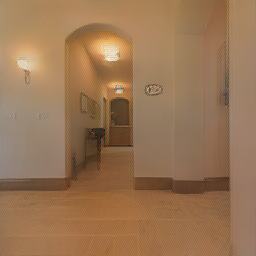
\includegraphics[width=0.24\textwidth]{images/implicitdoor1.png}
		\hfill
		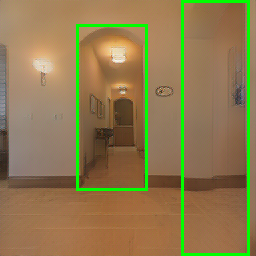
\includegraphics[width=0.24\textwidth]{images/implicitdoor1boxed.png}
		\hfill
		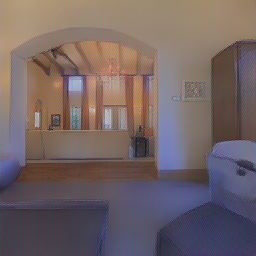
\includegraphics[width=0.24\textwidth]{images/implicitdoor2.png}
		\hfill
		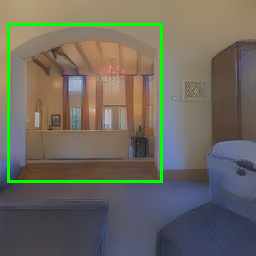
\includegraphics[width=0.24\textwidth]{images/implicitdoor2boxed.png}
		\caption{Implicit internal open doors and the relative bounding boxes.}
	\end{subfigure}
	
	\begin{subfigure}[b]{\linewidth}
		\centering
		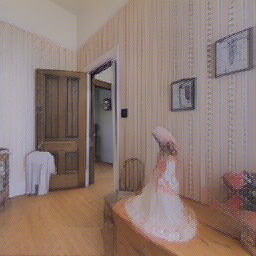
\includegraphics[width=0.24\textwidth]{images/explicitinternalopen1.png}
		\hfill
		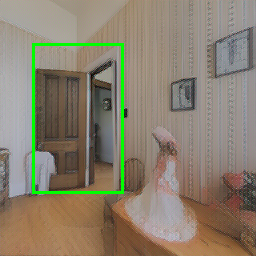
\includegraphics[width=0.24\textwidth]{images/explicitinternalopen1boxed.png}
		\hfill
		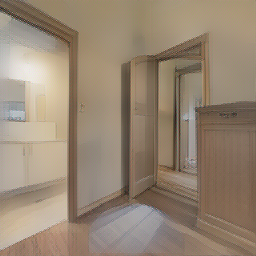
\includegraphics[width=0.24\textwidth]{images/explicitinternalopen2.png}
		\hfill
		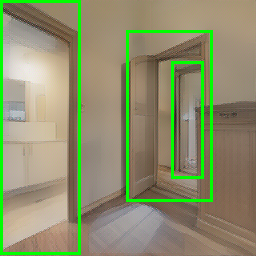
\includegraphics[width=0.24\textwidth]{images/explicitinternalopen2boxed.png}
		\caption{Explicit internal open doors and the relative bounding boxes.}
	\end{subfigure}
	
	\begin{subfigure}[b]{\linewidth}
		\centering
		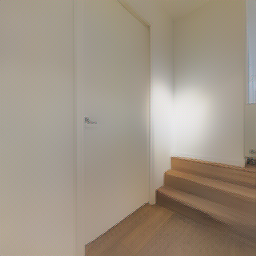
\includegraphics[width=0.24\textwidth]{images/explicitinternalclosed1.png}
		\hfill
		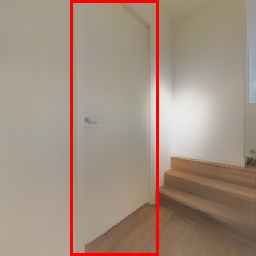
\includegraphics[width=0.24\textwidth]{images/explicitinternalclosed1boxed.png}
		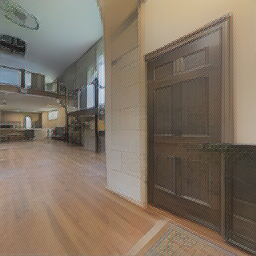
\includegraphics[width=0.24\textwidth]{images/explicitinternalclosed2.png}
		\hfill
		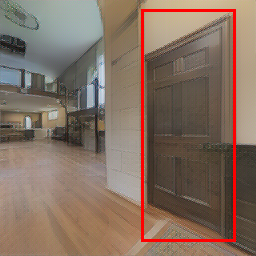
\includegraphics[width=0.24\textwidth]{images/explicitinternalclosed2boxed.png}
		\caption{Explicit internal closed doors and the relative bounding boxes.}	
	\end{subfigure}
	
	\begin{subfigure}[b]{\linewidth}
		\centering
		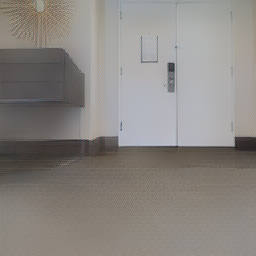
\includegraphics[width=0.24\textwidth]{images/explicitexternalclosed1.png}
		\hfill
		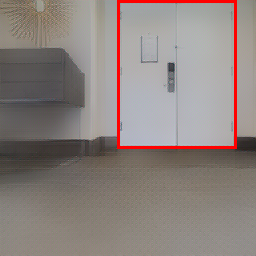
\includegraphics[width=0.24\textwidth]{images/explicitexternalclosed1boxed.png}
		\hfill
		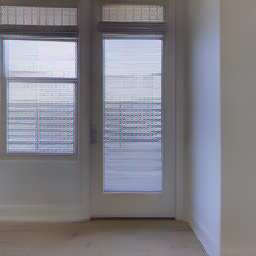
\includegraphics[width=0.24\textwidth]{images/explicitexternalclosed2.png}
		\hfill
		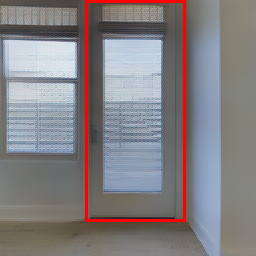
\includegraphics[width=0.24\textwidth]{images/explicitexternalclosed2boxed.png}
		\caption{Explicit external closed doors and the relative bounding boxes.}
	\end{subfigure}
	\caption{Different types of doors with ground truth bounding boxes. Green bounding boxes represent open doorways while red rectangles denote closed doors. These images are taken from Matterport3D \cite{matterport} environments simulated by Gibson \cite{gibson}.}
\end{figure}

\section{Proposed Solution}
\label{sec:solution}
In this thesis, we face the problem of door detection in autonomous mobile robots. In the following paragraphs, we expose the proposed solutions about the three main problems this work addresses: how to build the doors detector, how to improve the module's performance, and how to compose and evaluate a visual dataset in a robotic vision context.

\subsection{Build the Doors Detector Module} At first, we reduce to problem of finding doors in indoor environments to a well-known Computer Vision task: object detection in RGB images. After a literature review about this subject, we propose a module to detect doors based on DETR (DEtection TRansformer) \cite{detr}, a deep end-to-end architecture that performs object detection exploiting the Transformers' peculiarities \cite{transformer}. DETR views object detection as a direct set prediction problem, removing the need for many hand-designed components (like non-maximum suppression or anchor generation) that explicitly encode prior knowledge about the task. Thanks to the novel Transformer's architecture, DETR extract features from a frame and then finds the pair-wire relations between them. In this way, it reasons about the entire image as context. The authors demonstrate that DETR accuracy and run-time performance are comparable to the well-established and highly-optimized Faster R-CNN baseline \cite{fasterrcnn} on the challenging COCO object detection dataset \cite{coco}. 

We choose DETR because it approaches the object detection task as a direct set prediction problem, reasoning about the entire image as a context. Furthermore, this model has a simple architecture that can be implemented in any deep learning framework that provides a common CNN backbone and a transformer architecture. This means that it can be easily customized. Despite this, DETR is an enormous network with tens of millions of parameters and it is extremely data-hungry: the authors train DETR for 300 epochs with COCO's examples randomly modified with data augmentation procedures (e.g. resize, crop, scale, etc.). Due to this fact, we do not retrain DETR from scratch but we build our doors detector starting from its pre-trained version provided by the authors. We use the standard architecture reported in the original article \cite{detr}, modifying also the object queries hyper-parameter, called $N$. It indicates the maximum number of objects contained in a single image. The author set $N = 100$, but, in the experimental phase, we argue that this value is too high with respect to our doors dataset, in which an image contains at most 4 doors instances. For this reason, we set $N = 10$. This thesis demonstrates the versatility of DETR with respect to other object detection tasks, even with smaller datasets than COCO. This is done by evaluating DETR on a well-known doors dataset, DeepDoors2 \cite{deepdoors2}, and on a visual doors dataset collected in the context of this thesis.

\subsection{Increase the Detector's Performance} Another goal of this thesis is to improve the doors detector's accuracy. To address this problem, we do not focus on the deep module that performs object detection, but we reason about its context of use. We focus on a typical deployment scenario for indoor mobile robots (as described in Sec. \ref{sec:deploymentscenario}). We argue that, often, a robot is deployed in a single environment and works inside it for a long time. Furthermore, thanks to  the wayfinding principles described in Sec. \ref{sec:goals}, different views from the same indoor scene present a coherent visual aspect. This is also true for doors: a single environment presents a few types of doors that are repeated in multiple locations. The method to increase the doors detector's accuracy exploits these intuitions. Our approach, called \textbf{one-shot incremental learning}, aims to specialize the model for working in a precise environment using the fine-tune technique. 

Fine-tuning on pre-trained ImageNet classification models \cite{verydeepimagenet, resnet} has achieved impressive results for tasks such as object detection \cite{fasterrcnn, yolo, yolov2} and is becoming the common way for solving computer vision problems. Fine-tuning is a simple and effective
approach for transfer learning: it concerns training a deep model with common large datasets (such as ImageNet \cite{imagenet} or Microsoft COCO \cite{coco}). Then, the pre-trained model is re-trained with a few new data to solve a more refined task. In this way, the network's weights are set using a source dataset with a large number of examples provide a better
model initialization than random initialization. This is useful to speed up the training, overcome small dataset size, or prevent overfitting. We use the same principle to increase the performance of the proposed doors detector. 

In our approach, called \textbf{one-shot incremental learning}, the doors detector we proposed is initially trained with a general visual doors dataset, which can be downloaded from the internet or collected in some real or simulated environments. The resulting module is a general door detector that can be deployed in any environment. Then, the general detector (built using DETR) is fine-tuned using multiple sub-sets (with different sizes) of new unseen data acquired directly in the new scene. In this way, the general door detector specializes itself using new examples for increasing its performance in a precise environment. Since the fine-tune is performed using multiple sub-sets with different sizes of new data, we also investigate the number of unseen examples necessary to obtain a significant performance improvement.

\subsection{Compose and Evaluate the Visual Dataset}
This thesis address a Robotic Vision task that completely differs from Computer Vision application. As reported in \cite{surveydeeplimits}, perception is only one part of a more complex, embodied, active, and goal-driven system in robotics.
In a simplified view, whereas Computer Vision takes images and translates them into information, Robotic Vision translates images into actions. Furthermore, an autonomous agent operates in open-set conditions. A module used by a robot can assign high-confidence scores to unknown objects or falsely recognize them as one of the known classes. 

In order to understand how the doors detector performs in different environments, this thesis proposes a method to acquire a dataset of RGB images through simulation. We collect both positive images (that contain doors to detect) and negative frames (that do not depict objects of interest) from multiple scenes. We use Gibson \cite{gibson} to simulate an agent and its visual perception in environments taken from the Matterport3D worlds dataset \cite{matterport}. A mobile robot navigates in an environment following an exploration strategy, avoiding going too close to walls, furniture, and obstacles in general. Furthermore, a robot perceives the environment from different points of view, according to its position in the scene and the height of the camera. To take this fact into account, we propose an approach to select the different locations from which to acquire the data. This method, based on the work presented by \citeauthor{repeatabilityslamarxiv} \cite{repeatabilityslamarxiv, repeatabilityslam}, computes the Voronoi Graph of the occupancy grid maps of an environment. The locations from which to acquire the RGB images are chosen by sub-sampling the Voronoi Graph with a distance value. Thank to this algorithm, the doors dataset is acquired simulating a possible exploration strategy, avoiding collecting wrong or noise images that can degrade the model accuracy.

             % Kick-Off
\chapter{System Detail}

In this chapter, we define in detail the system we develop to solve to implement the method described Sec. \ref{sec:solution}. The system is composed of five main modules and each of them addresses a specific requirement imposed by our solution. We report the functionalities of each module, describing also the algorithms we implement and the technologies used for their construction. These modules are the following:

\begin{enumerate}
	\item \textbf{Doors Detector:} this module implements the main requirement of this thesis: the development of a doors detector for indoor autonomous robots. We approach the problem of finding doors as an object detection task, that we address using a deep learning technique. Doors detector is implemented through DETR \cite{detr}, a deep end-to-end architecture to perform object detection. To better understand how DETR works, we provide an overview of the principal machine learning and deep learning principles. Finally, we described in detail the DETR's architecture. 
	\item \textbf{Simulation Environment:} the second part of our system is the simulation environment used to collect the dataset. As described in Sec. \ref{sec:importanceofsimulation}, simulation is widely used in robotic applications, and, as explained in Sec. \ref{sec:goals}, this thesis address lack of suitable datasets for robotic applications. We use simulation to collect the dataset for training the doors detector. We choose Gibson \cite{gibson} as the virtualization framework and Matterport3D \cite{matterport} as the worlds' dataset. In the dedicated section, we describe the main functionalities of Gibson and Matterport3D. Then, we report the issues of these technologies that prevent correct and fast data collection. We finally explain the adopted solution to overcome these limitations: we developed a modified version of Gibson that implements a new simulation stage in which the robot can be placed freely in any location.
	\item \textbf{Pose Estimator:} this module emulates a possible navigation strategy used by a real autonomous agent and extracts  the locations from which the data points are collected. Thanks to this module unified with the new version of Gibson, we offer a method to easily acquire a suitable visual dataset for a robotic context. We report the underlying algorithms implemented in this component, which is inspired by the works proposed by \citeauthor{repeatabilityslam} in \cite{repeatabilityslam, repeatabilityslamarxiv}.
	\item \textbf{Dataset Manager:} another important aspect of the system provided by this thesis is the dataset. We report in detail by which data it is composed, describing also the labeling procedure. In addition, we mention the framework we developed for managing the dataset.
	\item  \textbf{Model Evaluator:} the last component of our system aims to evaluate the model's performance. As reported in Sec. \ref{sec:solution}, we propose a new metric that considers also the negative images (examples with no objects of interest). For this module, we describe the metric we propose and the procedure to obtain its results.
\end{enumerate}


\section{Doors Detector}
\label{sec:doors_detector}

The main goal of this thesis is to propose a doors detector that is able both to find doors within RGB images and understand their status (open or closed). We reduce these problems to a precise Computer Vision task: object detection. The doors detector we propose is built with DETR \cite{detr}, a novel end-to-end deep module based on Transformers. The module we develop is public available on Github, in the main repository\footnote{The main thesis's repository: \url{https://github.com/micheleantonazzi/master-thesis-robust-door-detector}.} of this thesis inside the \textsf{doors-detector} package. Before talking about DETR and how it is used to detect doors, we review the most relevant aspects of the Deep Learning theory.

\subsection{Machine Learning Review}
\label{sec:machine_learning}
Deep Learning is a sub-field of Machine Learning, which is the study of computer algorithms that can improve automatically through experience by the use of data. We define the most important aspect of Machine Learning before talking about the proposed approach to detect doors. Machine Learning is a powerful technique suitable when it is not feasible to develop a standard algorithm to solve a difficult task. A \textit{learning algorithm} uses sample pairs of training data to create a model, also called predictor, that is able to classify other unseen data. The first important aspect for a machine learning problem is the dataset. Typically, a dataset is composed of pairs of data taken from two different domains: the \textit{data space} and the \textit{label set}.

\begin{definition}[Data domain]
	We use $X$ to denote the set of all possible data points for a given learning problem. Each data point is defined by features. In some cases, the features are encoded as vectors of real numbers. Such a vector representation is \textit{natural} whenever the data consist of homogeneous quantities, like pixels in an image or words' frequencies in a document. A data point is denoted as $x \in X$ and it is defined as a vector of feature $x = (x_1, ..., x_d)$.
\end{definition}

\begin{definition}[Label set]
	We use $Y$ to denote the set of all possible labels that a data point can assume. For a classification problem, the label set is typically finite and small (such as $Y = \{sport, policies, business\}$ for a documents categorization task). Otherwise, for a regression task, the label set is typically equal to $\mathbb{Q}$, which is the rational numbers' set. In this case, the label set is infinite.
\end{definition}

In a \textit{supervised} learning problem, the data points are tagged with their respective ground-truth labels. In particular, the dataset's entries are pairs $p = (x, y)$, where $x \in X$ is a data point and $y \in Y$ is the label assigned to it. A \textit{supervised} learning algorithm is a technique that aims to build a model learned from a \textit{training set}. This paradigm is called \textit{learning by examples}. An example is a pair $p=(x, y)$, where $x$ is a data point represented by a feature vector and $y$ is its ground-truth label, while the training set is composed of a series of examples $S=\{(x_1, y_1), ..., (x_m, y_m)\}$. A \textit{supervised learning algorithm} for \textit{learning by examples} receives a training set and outputs a learned model.

\begin{definition}[Model]
	A model is a function $f:X \to Y$ that maps data points to labels.
\end{definition}

The training examples come from some generally unknown probability distribution and the goal of a learning algorithm is to infer a function that approximates this distribution (or makes a generalization of it) to produce sufficiently accurate predictions in new cases. In order to estimate the predictive power of a model, we typically use a \textit{test set}. This is a set of examples $T=\{(x_1', y_1'), ..., (x_n', y_n')\}$ to which the learning algorithm does not have access during the training phase. 

During the training procedure, each pair in the \textit{test set} are fed into the model in order to measure the goodness of each prediction compared with the ground-truth label. This quantity is measured by the \textit{loss function}. Then, the prediction's error computed by the loss function is used to adjust the model's parameters in order to improve its accuracy. 

\begin{definition}[Loss function]
	A loss function $\ell(y, \hat y)$ measures the discrepancy between the predicted label $\hat y$ and the ground-truth label $y$. Typically, in a correct prediction the loss function's values is $0$: $\ell (y, \hat y) = 0$.
\end{definition}

The test set allows determining the predictive power of a learned model on unseen new data. To measure the goodness of a predictor, we can calculate the \textit{test error} over a test set $S$. Given a loss function $\ell$, the test error is
\begin{equation}
\frac{1}{n} \sum_{s=1}^{n}\ell(y_s', f(x_s'))
\end{equation}
where $n$ is the test set's cardinality ($n = |S|$), $y_s'$ is the ground-truth label of the s-th test example and $f(x_s')$ returns the label from the s-th data point produced by the predictor $f$. Since the test set is disjoint from the training set and emulates the unseen data, it cannot be used during the learning phase.

A way to train a learning model is the Empirical Risk Minimization (ERM) approach. ERM offers a theory to design learning algorithms that generate predictors with a low test error considering only the training set. ERM assumes that the \textit{training error} (the error computed over a training set $T$) of a predictor is directly correlated to its test error. The training error is given by:

\begin{equation}
\hat \ell(f) = \frac{1}{m} \sum_{t=1}^{m}\ell(y_t, f(x_t))
\end{equation}
where the $m$ is the training set's cardinality ($m = |T|$).

\begin{definition}[Empirical risk minimization] 
	Let $\mathcal{F}$ a set of predictors and $\ell$ a loss function. The empirical risk minimizer (ERM) is the learning algorithm that outputs some predictor in $\mathcal{F}$ minimizing the training error
	
	\begin{equation}
	\hat f \in \argmin_{f \in \mathcal{F}} \hat \ell(f).
	\end{equation}
	The notation $\in$ denotes there could be multiple $f \in \mathcal{F}$ that minimize the training error.
\end{definition}

The ERM algorithm fails when no predictors in $\mathcal{F}$ have a low test error, in particular when 

\begin{equation}
	\min_{f \in \mathcal{F}} \frac{1}{n} \sum_{s = 1}^{n} \ell(y_s', f(x_s'))
\end{equation} 
is high. The two main ways of failing for a generic learning algorithm are:
\begin{itemize}
	\item \textbf{underfitting:} when a learning algorithm tends to outputs predictors whose both test and training errors are high and close to each other. This means that possible predictors are unable to correctly classify the samples in the training set as well as those in the test set. This situation could depend on the training test size: if it is too small it can not represent well the data points' distribution or $\mathcal{F}$ (the set of the possible predictors) are too large with respect to the training set dimensions. Another reason that causes underfitting is the cardinality of $\mathcal{F}$. If the set of the possible predictors is small, there could not be a subset of them with a small test error. This means that the learning algorithm is not complex enough to output good learned models. In other words, when a model underfits it is not able to represent well the problem, failing to classify examples from both training and test sets;
	\item \textbf{overfitting:} when a learning algorithm tends to output predictors whose training error is low (or it tends to zero) while the test error is high. In this situation, the predictors produced by a learning algorithm learn too much from the training data and, as a result, are unable to produce good predictions on new data. This means that those predictors do not generalize the problem, but are specialized in dealing only with the data used during the training phase.
\end{itemize}

When $A$ is an ERM learning algorithm and the size $m$ of the training set is fixed, we should expect overfitting when $\log_2|\mathcal{F}| \gg m$, so the set of possible predictors is too large with respect to the training set's size. On the other hand, when $\log_2|\mathcal{F}| \ll m$ we should expect underfitting.

\subsection{Deep Learning Review}
Deep Learning is a sub-field of Machine Learning based on \textit{neural networks}. This learning algorithm is inspired by the information processing and the distributed communication of biological brains. Neural networks (NNs) are a large and complex class of predictors, based on artificial neurons.

\begin{definition}[Neuron]
	An artificial neuron is a mathematical function inspired by biological neurons, which represents the elementary units in an artificial NN. The mathematical function implemented by a neuron is $g(x) = \sigma(\omega^\intercal \cdot x)$, where $\sigma$ is the activation function, $\omega$ is the weight vector of the learnable parameters, and $x$ is the input vector of the neuron. This means that each input is separately weighted and the sum is passed through a non-linear function. The activation function usually has a sigmoid shape and often it is monotonically increasing, continuous, and bounded. A single neuron can approximate only linear functions.	
\end{definition}

Artificial neural networks are composed of a series of simple predictions made by neurons. The adjective ``deep'' in Deep Learning refers to the use of multiple layers in NNs. The most simple model of neural networks is feed-forward NNs. 

\begin{definition}[Feed-forward neural network]
A feed-forward neural network computes functions of the from $f : \R^d \to \R^n$. Its structure is a directed acyclic graph $G = (V, E)$, in which $V$ is the set of nodes (neurons) and $E$ is the set od edges that connects the neurons. The presence of multiple neurons allows the neural network to infer non-linear functions. The vertices in $V$ are divided into three subgroups: $V = V_{in} \cup V_{hid} \cup V_{out}$, where $V_{in}$ (with $|V_{in}| = d$:	 the feature space's dimension) are the input nodes which have no incoming edges, $V_{out}$ (with $|V_{out}| = n$, the number of labels) are the output nodes which have no outgoing edge, and $V_{hid}$ are the hidden nodes, which have both incoming and outgoing edges.
\end{definition}

The most simple form of the feed-forward neural network is the multi-layer perceptron (MLP), in which the nodes of $V$ is partitioned in a sequence of consecutive layers such that each node of a layer has incoming edges only from
nodes in the previous layer and outgoing edges only to nodes of the next layer.  The layers containing the hidden nodes are called hidden layers. 

\begin{figure}[h!]
	\centering
	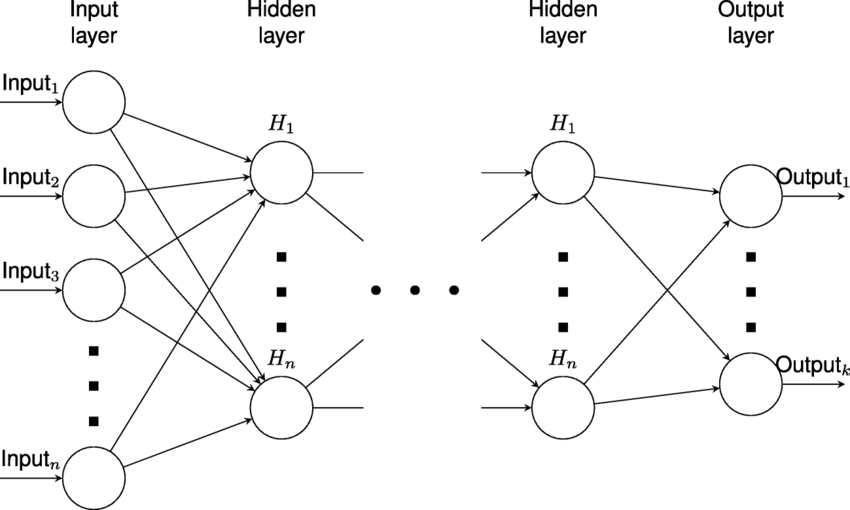
\includegraphics[width=0.85\linewidth]{images/mlp.png}
	\caption{An example of a multi-layer perceptron, with $d$ input nodes and $n$ output nodes. In this example, the connectivity between layers is complete (there are no missing edges).}
\end{figure}

The learnable parameters are the weights assigned to the edges between neurons. 
A parameter $\omega_{i,j} \in \R$ (called weight) is associated with every edge pair $(i, j) \in E$.  We use $W$ to denote the $|V | \times |V |$ weight matrix, where $(i, j) \notin E$ implies $\omega_{i,j} = 0$. The graph $G$, the weights matrix
$W$, and the activation function $\sigma$ define the function $f = f_{G,W,\sigma}$ computed by the network.  Note that when $n = 1$ (one output node) and $|V_{hid}| = 0$ (no hidden nodes), then $F_{G,\sign}$ only contains linear classifiers of the form $f(x) = \sign(\omega^\intercal \cdot x)$. The training of neural networks is not trivial. The most natural approach for training a model in $\mathcal{F}_{G,\sigma}$ is ERM, as mentioned in Sec. \ref{sec:machine_learning}.
Unfortunately, this method could not be efficiently applied to neural networks. 

\begin{theorem}
	For every integer $k \geq 3$, let $G$ be a network with $d$ input nodes, a single hidden layer containing $k + 1$ nodes (one of which has a constant value 1), and a single output node. Then the problem of minimizing the zero-one loss training error in $\mathcal{F}_{G,\sign}$ is NP-hard. 
\end{theorem}

The models considered by this theorem are simplified neural networks to solve a \textit{binary classification} task using the zero-one loss (equation \ref{formula:zero-oneloss}) with a single hidden layer composed of four or more neurons. 

\begin{equation}
	\label{formula:zero-oneloss}
	\ell(y, \hat y) = 
	\begin{cases}
	0 & \text{if $y = \hat y$} \\
	1 & \text{if $y \neq \hat y$}
	\end{cases}
\end{equation}

This theorem demonstrates the inefficiency of ERM for a simple NN. This means that this theorem is true even for more complex neural networks and different tasks. ERM remains NP-hard even when $\mathcal{F}_{G,\sign}$ contains only linear classifiers (i.e., $G$ has no hidden nodes). However, while the cause of NP-hardness in linear models was the non-convexity of the loss function (zero-one loss in this case), in multi-layered neural networks the problem is inherent to their structure. The key observation is that the presence of hidden nodes in NN makes the loss function $\ell_t$ over an example $(x_t, t_t)$ non-convex in the weights matrix $W$ even when $\ell(x, y)$ is convex for all $y$. In general, the problem of minimizing a non-convex function is computationally intractable.  

This is because NNs are successfully trained using algorithms that reduce the training error without any mathematical guarantee on the solution's quality. The training procedure starts with a forward propagation of the training examples in the neural network. After that, the outputs are used to quantify how good the predictions are and the error are back-propagated in the network using a descent algorithm. The standard training algorithm for NNs is stochastic gradient descent (SGD):

\begin{equation}
\omega_{i, j} \leftarrow \omega_{i, j} - \eta_t \frac{\partial\ell_{Z_t}(W)}{\partial\omega_{i, j}} \quad \quad (i, j) \in E,
\end{equation}
where $Z_t$ is the index of a random training example and $\eta$ is an hyper-parameter that controls the step size (also called learning rate). The main idea is to calculate the partial derivative of the loss function, calculated on a training data point $t$ and the current NN status (described by the weights matrix $W$), over all the learnable parameters to adjust their values. In order to speed up convergence, the training samples can be grouped in mini-batches. Because the training error is a non-convex function of $W$, the SGD algorithm essentially finds only a local minima of the training error. The procedure to perform gradient descent on feed-forward NNs is known as \textit{error back-propagation}. 

\subsection{DETR}
\label{sec:detr}
The doors detector proposed by this thesis is based on DETR \cite{detr} (DEtection TRansformer), a novel deep approach to perform object detection.  In DETR, the object detection problem is modeled as a direct \textit{set prediction}, making the detection pipeline a simple end-to-end unified architecture. Modern detectors address this set prediction in an indirect way using hand-crafted algorithms based on a large set of proposals \cite{yolo} or anchors \cite{focalloss}. Their performances are significantly influenced by these post-processing steps to collapse near-duplicate predictions, like non-maximum suppression or anchor generation. The first important aspect of DETR  is its architecture (explained in Sec. \ref{sec:detrarchitecture}). DETR uses a Transformer to find complex relationships between features extracted in the same image. In this way, the model reasons about the whole image context without considering any form of prior knowledge about the task. The second important aspect to address the set prediction problem is the loss functions (described in \ref{sec:detrlosses}). DETR uses a set loss function that performs bipartite matching between predicted and ground-truth objects.

\subsubsection{DETR Architecture}
\label{sec:detrarchitecture}
The architecture of DETR (reported in Fig. \ref{fig:detrarchiecture}) consists of three main components: a backbone convolutional neural network (CNN) for features extraction, an encoder-decoder transformer to capture the relationships between the extracted features, and a simple feed-forward network (FFN) that makes the final detection prediction (the coordinates of the bounding boxes and their relative labels).

\begin{figure}[h!]
	\centering
	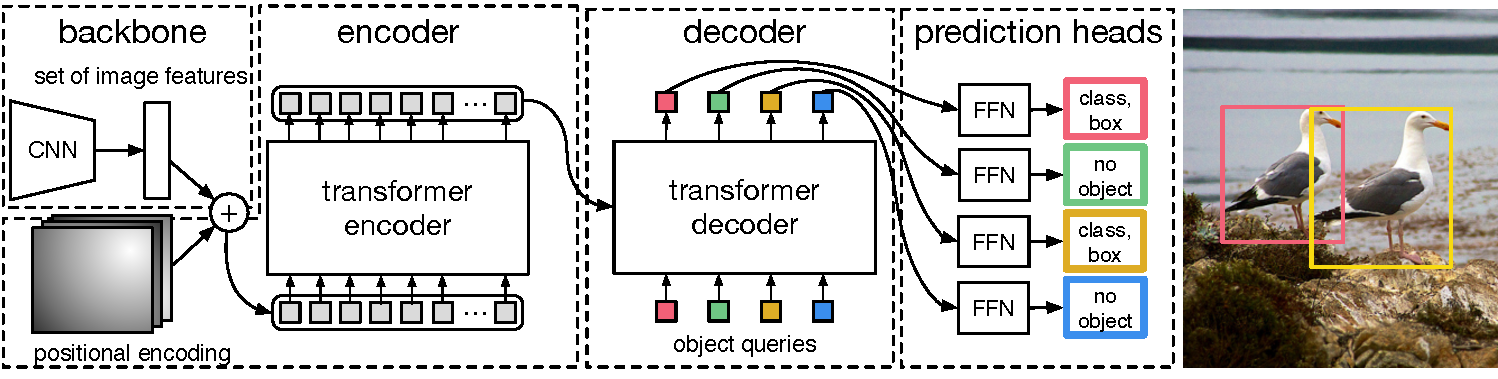
\includegraphics[width=\linewidth]{images/detrarchitecture.pdf}
	\caption{The architecture of DETR. It uses a conventional CNN backbone to learn a 2D representation of an input image. Then, this representation is flattened and encoded before being passed into the transformer encoder. The transformer decoder then takes as input a small fixed number of learned positional embeddings, called \textit{object queries}, and additionally attends to the encoder output. Finally, each output embedding of the decoder is processed by a  simple feed-forward network (FFN) that predicts either a detection (class and bounding box) or a ``no object'' class. Image from \cite{detr}.}
	\label{fig:detrarchiecture}
\end{figure}

\paragraph{CNN Backbone} The first element in DETR's architecture is a CNN backbone.  Ideally, any backbone can be used depending upon the complexity of the task to provide a low dimensional representation of the image extracting features from it. Starting from the initial image $x_{img} = \R^{3\times H_0\times W_0}$ (with 3 color channel and dimension $H_0$, $W_0$), a conventional CNN backbone generates a lower-resolution activation map $f \in \R^{C \times H \times W}$. Typical values used in this paper are $C = 2048$ and $H, W = \frac{H_0}{32}, \frac{W_0}{32}$. 

The authors use a ResNet (residual network) \cite{resnet} as CNN backbone, a neural network that solves the issue of vanishing gradient. This problem makes a deeper neural network more difficult to train and optimize: when a network's depth increases, accuracy gets saturated and then degrades rapidly. This unwanted situation is called \textit{degradation} (of training accuracy). Unexpectedly, such degradation is not caused by overfitting, and adding
more layers to a deep model leads to higher training error. The authors address the degradation problem by introducing a \textit{deep residual learning} framework, commonly called ResNet. The proposed method is based on the insight that a few overlapping layers can fit a residual mapping instead of directly fitting a desired underlying mapping. This principle is formalized as follows. Let $\mathcal{H}(x)$ be the desired underlying mapping fit by a few stacked layers (not necessarily the entire net), where $x$ denotes the inputs of the first layer. Since multiple non-linear layers can approximate non-linear functions, then  the same layers can approximate the residual functions $\mathcal{H}(x) - x$. The authors let these layers approximate a residual function
$\mathcal{F}(x) := \mathcal{H}(x) - x$, so the original function becomes
$\mathcal{F}(x)+x$. The authors hypothesize that it is easier to optimize the residual mapping than to optimize the original unreferenced mapping.  If the optimal function is closer to an identity
mapping than to a zero mapping, it should be easier for the
solver to find the perturbations with reference to an identity
mapping, than to learn the function as a new one. This means that subsequent blocks in our network are thus responsible for fine-tuning the output of a previous block, instead of having to generate the desired output from scratch.

\begin{figure}[h!]
	\centering
	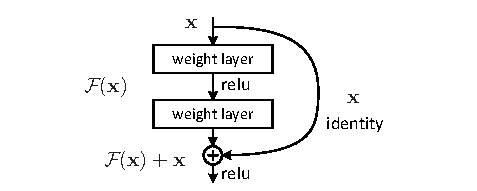
\includegraphics[width=\linewidth]{images/residualblock.pdf}
	\caption{Residual learning: a building block. The formulation of $\mathcal{F}(x)+x$ can be realized with a ``shortcut connection'', that skips one or more layers. Image from \cite{resnet}.}
	\label{fig:resblock}
\end{figure}

\paragraph{Transformer Encoder-Decoder} The second part of DETR is a Transformer \cite{transformer}, a novel sequence-to-sequence (Seq2Seq) architecture that transforms a given sequence of elements, such as the sequence of words in a sentence, into another sequence. Seq2Seq models are particularly useful for natural language process tasks (NLP), text classification, machine translation, and
question answering. Among their salient benefits, Transformers enable modeling long dependencies between input sequence elements, support parallel processing, and require minimal inductive biases for their design. Recent studies \cite{surveytransformer} demonstrate the application of Transformer in Computer Vision. By using a Transformer model, DETR globally reasons about all objects together using pair-wise relations between them and being able to use the whole image as context. In this way, DETR predicts (in a single pass) a set of objects and
models their relations. Since DETR performs object detection, the Transformer's input is a sequence of features extracted from an image.

The Transformer model, proposed by \citeauthor{transformer} \cite{transformer}, is the first transduction model relying entirely on self-attention mechanism to compute representations of its input and output without using RNNs or convolutions. Self-attention, sometimes called intra-attention, is an attention mechanism that relates every single element in a sequence with the other elements and finally computes a representation of the entire sequence. In other words, the attention mechanism decides at each step which parts of the sequence are important by assigning a weight to each element. The Transformer architecture (Fig. \ref{fig:transformerarc}) is based on an encoder-decoder structure. In a general way, the encoder maps an input sequence of symbol representations $(x_1, ..., x_n)$ into a sequence of continuous representations $z = (z_1, ..., z_n)$. Given $z$, the decoder then generates an output sequence $(y_1, ..., y_m)$ of symbols one element at a time.

More specifically, the Transformer's encoder  is composed of a stack of $N = 6$ identical layers. Each layer has two sub-layers: the first is a multi-head self-attention mechanism and the second is a simple, position-wise fully connected feed-forward network. The authors add a residual connection (like ResNet \cite{resnet}) around each sub-layer, followed by layer normalization. The output of each sub-layer is $\text{LayerNorm}(x + \text{Sublayer(x)})$. The decoder is also composed of a stack of $N = 6$ identical layers. Each of them has the same sub-layers of the encoder with a third one that performs multi-head attention over the output of the encoder stack. The authors modify the self-attention
sub-layer in the decoder to prevent positions from attending to subsequent positions. This masking, combined with fact that the output embeddings are offset by one position, ensures that the predictions for the position $i$ can depend only on the known outputs at positions less than $i$.

\begin{figure}[h!]
	\centering
	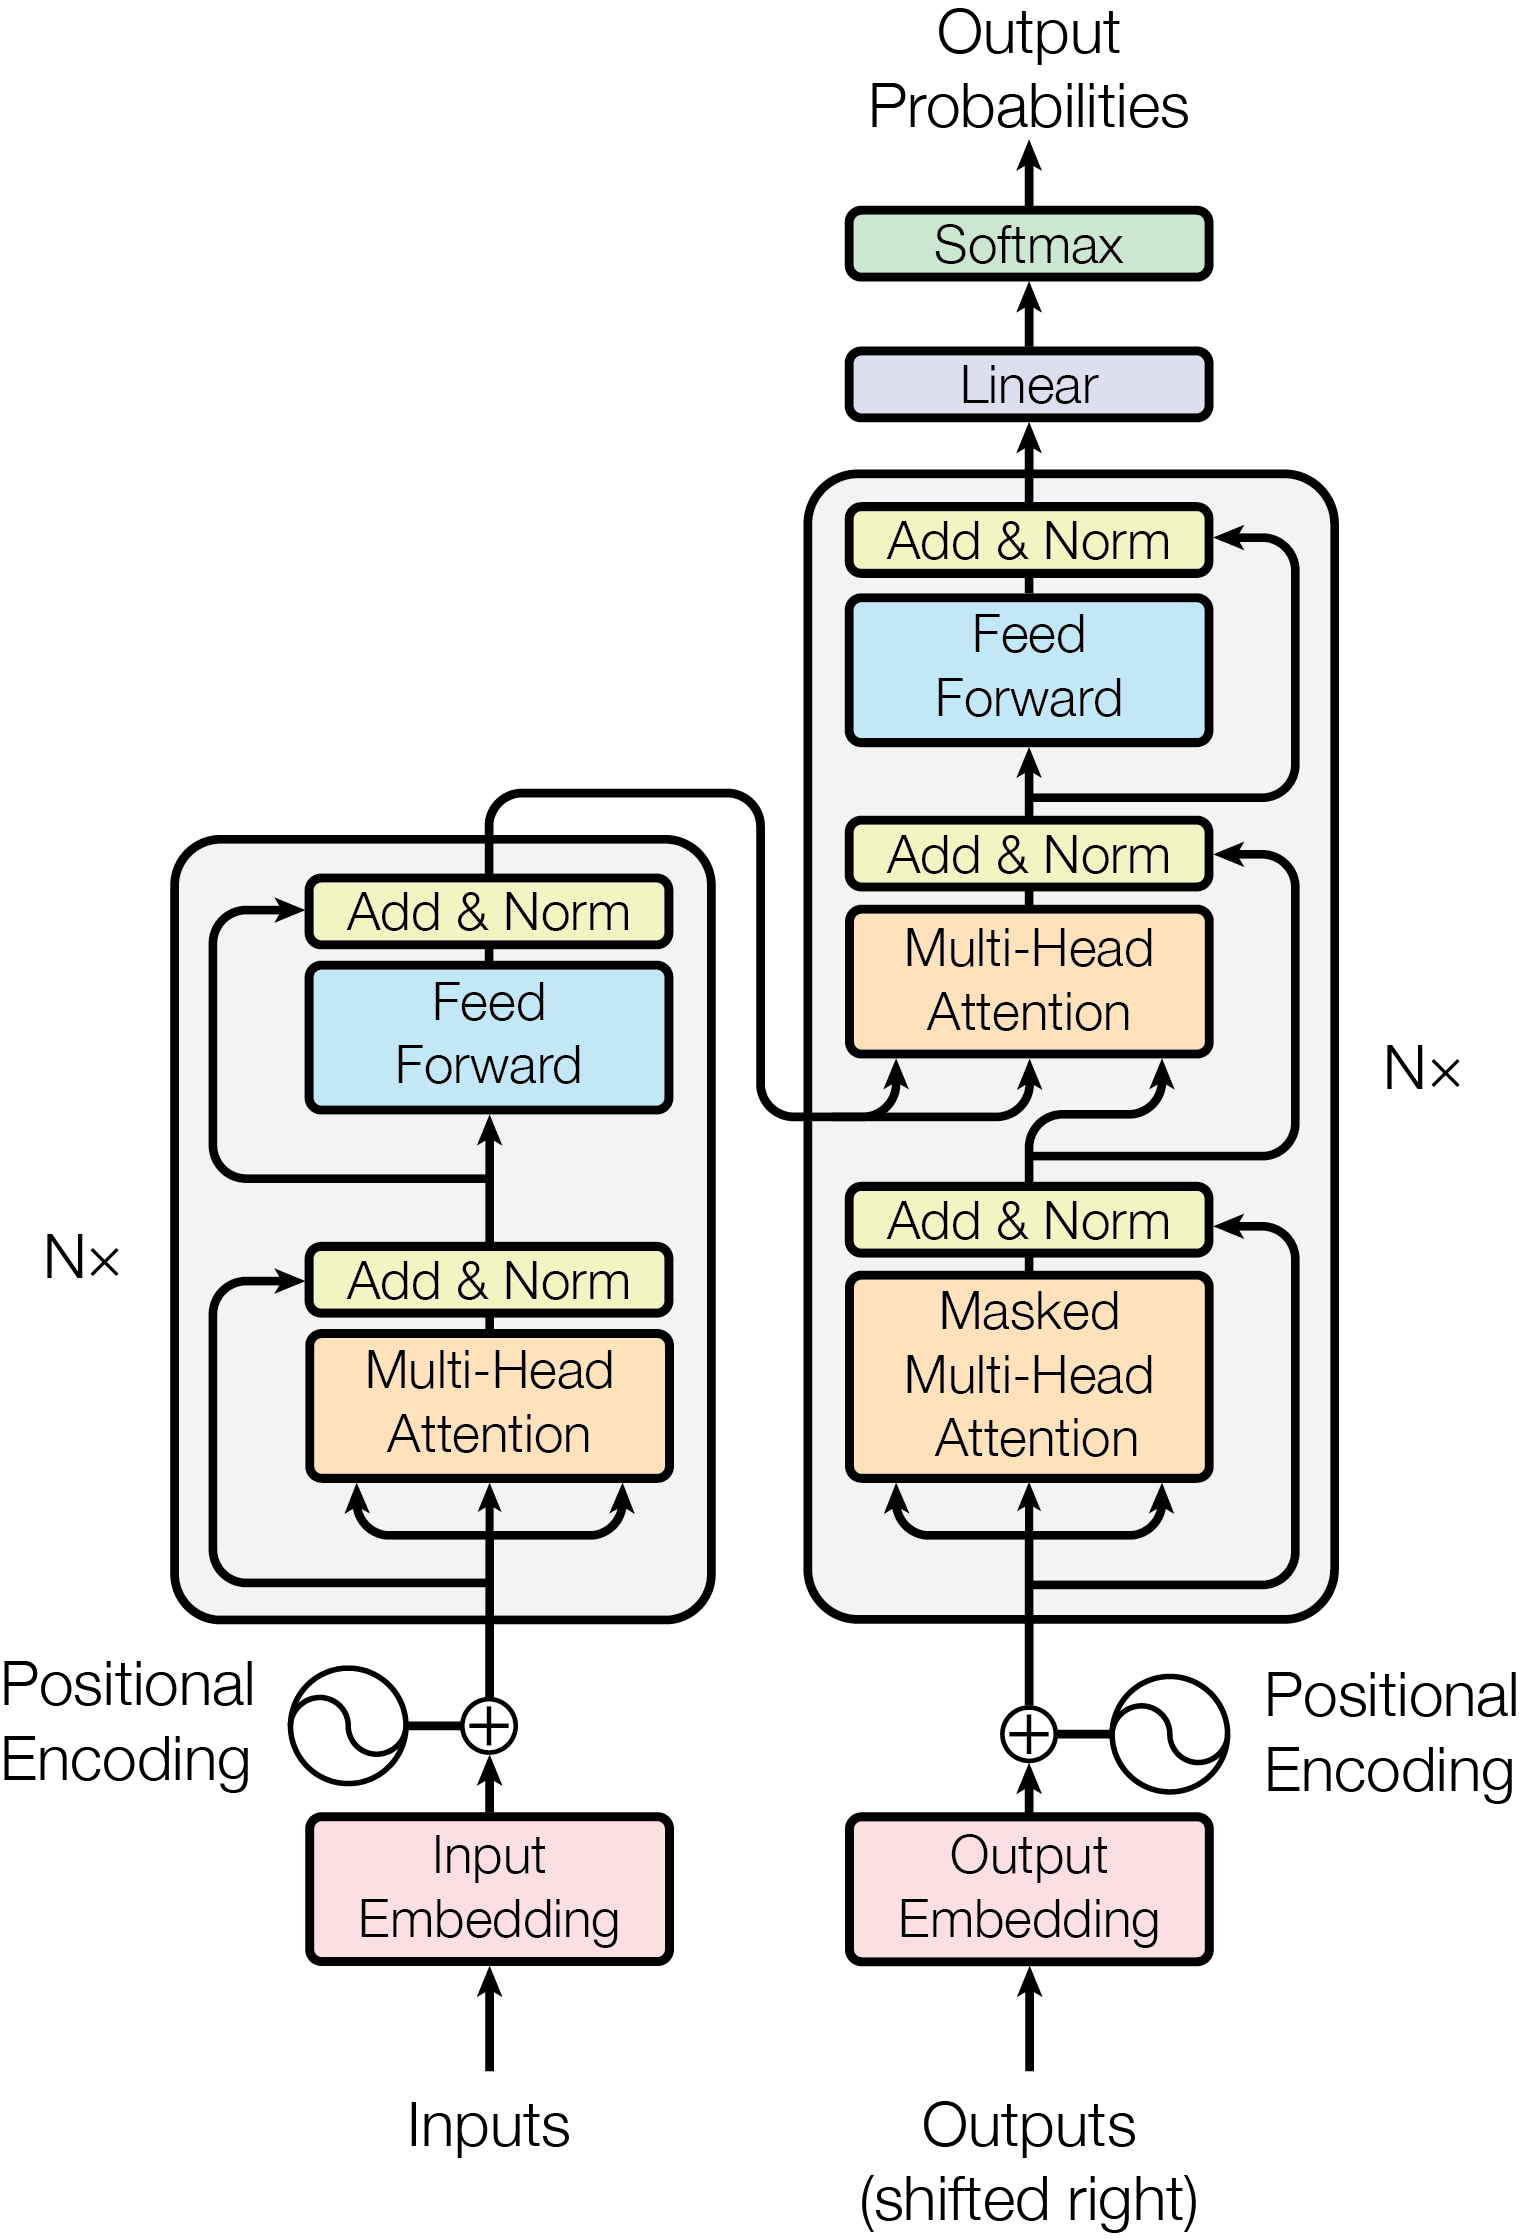
\includegraphics[width=0.8\linewidth]{images/transformerarchitecture.png}
	\caption{The Transformer model architecture. Image from \cite{transformer}.}
	\label{fig:transformerarc}
\end{figure}

DETR \cite{detr} uses a standard Transformer developed for natural language process as proposed in \cite{transformer}. The high-level activation map $f$ extracted from the CNN backbone is rescaled from $C$ to a smaller dimension $d$ by a $1\times1$ convolution. The new feature map fed into the Transformer's encoder is $z_0 \in \R^{d, H, W}$. Since the encoder requires a sequence as input, the feature map $z_0$ is collapsed the spatial into one dimension, resulting in a $d\times HW$ feature map. The decoder transforms $N$ embeddings of size $d$.  The difference with the original Transformer \cite{transformer} is that DETR decodes the $N$ objects in parallel at each decoder layer. These input embeddings (called \textit{object queries}) are positional encoding vectors learned by the model during the training phase. They are passed to the input of each attention layer. Since the decoder is permutation-invariant, the $N$ input embeddings must be different to produce different results. Each object query is transformed into an output embedding by the decoder. The number of object queries is a hyper-parameter and it must be greater than the quantity of different objects in an image.

\paragraph{Feed-Forward Networks} The $N$ object queries produced by the decoder are  independently classified into box coordinates and class labels by
a feed-forward network, resulting in $N$ final object predictions. The final predictor is composed of a 3-layer perceptron and a linear projection layer. The perceptron predicts the normalized center coordinates, height, and width of the bounding boxes while the linear layer predicts the class labels. Since DETR predicts a
fixed-size set of $N$ bounding boxes, where $N$ is much larger than the
actual number of objects of interest in an image, an additional special class label $\varnothing$ is used to represent that no object is detected within a slot (it indicates the ``background'' class).

\subsubsection{DETR Loss Functions}
\label{sec:detrlosses}

DETR \cite{detr} simplifies the detection pipeline by dropping multiple hand-designed components that encode prior knowledge, like spatial anchors or non-maximal suppression. To address set prediction in a fully end-to-end way, DETR uses a novel loss function, called \textit{object detection set prediction loss}, that produces
optimal bipartite matching between predicted and ground-truth objects, considering both the class labels and the bounding boxes.

\paragraph{Object Detection Set Prediction Loss} DETR \cite{detr} infers a fixed-size set of $N$ predictions through the $N$ object queries produced by the Transformer's decoder. It is important that $N$ is significantly larger than the maximum number of objects in every image. One of the main difficulties of training is to score predicted objects, by considering the class, position, and size, with respect to the ground-truth. The authors propose a loss function that produces
an optimal bipartite matching between predicted and ground-truth objects considering object-specific (bounding box) losses. 

\begin{figure}[h!]
	\centering
	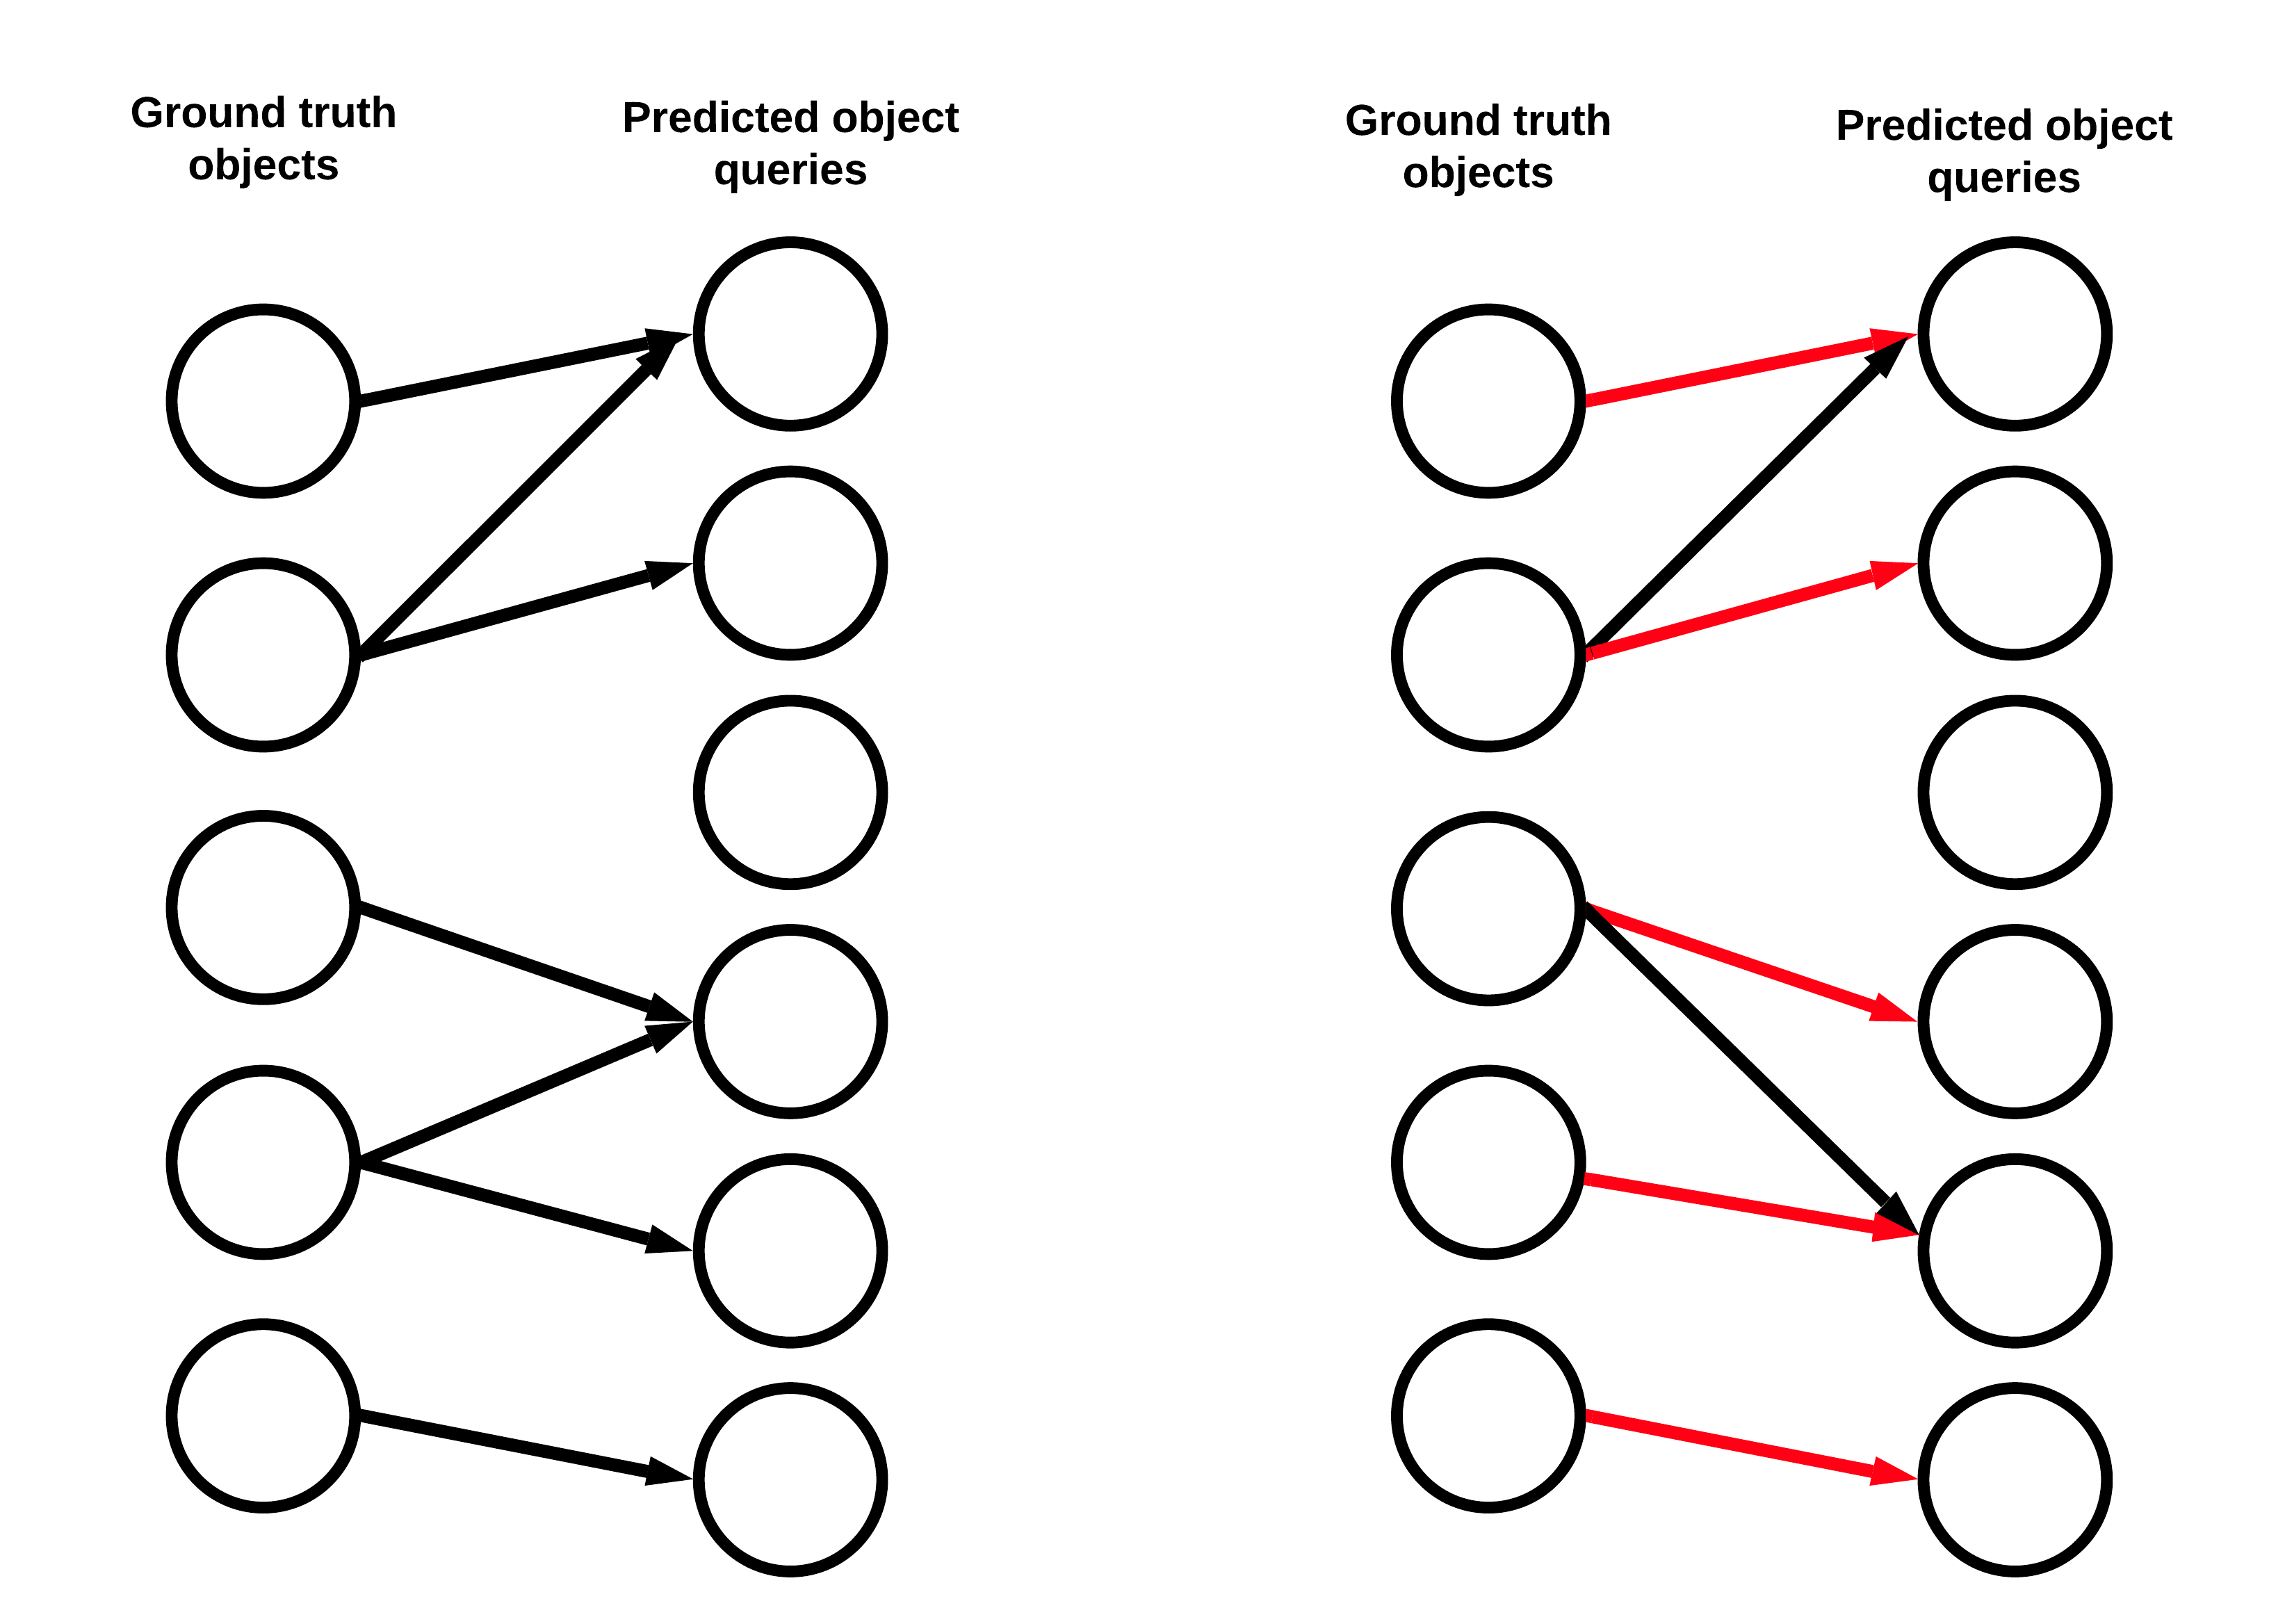
\includegraphics[width=0.9\linewidth]{images/bipartitematching.png}
	\caption{A matching in a bipartite graph. It consists of a set of edges chosen in such a way that no two edges share an endpoint. The loss function $\hat \sigma$ (Eq. \ref{formula:bipartitematching}) finds the best match with the lowest cost between the predicted bounding boxes and the ground-truth objects.}
	\label{}
\end{figure}

Let $y$ be the ground-truth set of objects, and $\hat y = \{\hat y_i\}^{N}_{i = 1}$ the set of $N$ predictions. The bipartite matching between these two sets is the best permutation $\hat \sigma \in \mathcal{G}_N$ of $N$ elements with the lowest cost:

\begin{equation}
\label{formula:bipartitematching}
\hat \sigma = \argmin_{\sigma \in \mathcal{G}_N} \sum_{i}^{N} \mathcal{L}_{match}(y_i, \hat y_{\sigma(i)}),
\end{equation}
where $\mathcal{L}_{match}(y_i, \hat y_{\sigma(i)})$ is a pair-wise \textit{matching cost} between  ground-truth $y_i$ and a prediction with index $\sigma(i)$. This optimal assignment is computed efficiently
with the Hungarian algorithm \cite{hungarian}. The matching cost takes into account both the class prediction and the similarity between predicted and the ground-truth bounding boxes. Each element $i$ can be seen as $y_i = (c_i
, b_i)$, where $c_i$
is the target class label (which may be $\varnothing$) and $b_i \in [0, 1]^{4}$
is a vector that defines ground-truth box coordinates and dimensions. For the
prediction with index $\sigma(i)$, the probability of class $c_i$ is defined as $ \hat p_{\sigma(i)}(c_i)$ and
the predicted box as $\hat b_\sigma(i)$. Whit these notations, the authors define the matching cost as

\begin{equation}
	\mathcal{L}_{match}(y_i, \hat y_{\sigma(i)}) = -\mathds{1}_{\{c \neq \varnothing\}}\hat p_{\sigma(i)}(c_i) + \mathds{1}_{\{c \neq \varnothing\}}\mathcal{L}_{box}(b_i, \hat b_{\sigma(i)}),
\end{equation}
which performs one-to-one matching for direct set prediction without duplicates. 

The next step is to compute the loss function, called \textit{Hungarian loss}, for all pairs matched in the previous step. It is a linear combination of a negative log-likelihood for class prediction and a box loss defined later:

\begin{equation}
\mathcal{L}_{\text{Hungarian}}(y, \hat y) = \sum_{i = 1}^{N} \bigg [-\log \hat p_{\hat\sigma(i)}(c_i) + \mathds{1}_{\{c \neq \varnothing\}}\mathcal{L}_{box}(b_i, \hat b_{\hat\sigma(i)}) \bigg ]
\end{equation}
where $\hat \sigma$ is the optimal assignment computed in Eq. \ref{formula:bipartitematching}. In practice, the authors
down-weight the log-probability term when $c_i = \varnothing$ by a factor 10 to account for class imbalance. 

\paragraph{Bounding Box Loss} The second part of the matching cost in the Hungarian loss is $\mathcal{L}_{box}(\cdot, \cdot)$ that scores the bounding boxes. The authors perform box predictions directly without any initial guesses using the $\ell_1$ loss. In our context, this loss measures the distance between the  ground-truth bounding box ($b_i$) and the best predicted box ($\hat b_{\sigma(i)}$) through the L1 norm:

\begin{equation}
\ell_1(b_i - \hat b_{\sigma(i)}) = ||b_i - \hat b_{\sigma(i)}||_1.
\end{equation}

While such an approach simplifies the implementation, the $\ell_1$ loss will have different scales for small and large boxes even if their relative error is similar. To mitigate this issue, the final $\mathcal{L}_{box}(\cdot, \cdot)$ is a linear combination of the $\ell_1$ loss and the generalized IoU loss \cite{generalizediou} $\mathcal{L}_{iou}(\cdot, \cdot)$, that is scale-invariant. The final bounding box loss is:

\begin{equation}
\label{eq:bounding_box_loss}
\mathcal{L}_{box}(b_i, \hat b_{\sigma(i)}) = \lambda_{iou}\mathcal{L}_{iou}(b_i, \hat b_{\sigma(i)}) + \lambda_{L1}||b_i - \hat b_{\sigma(i)}||_1,
\end{equation}
where $\lambda_{iou}$ and $\lambda_{L1}$ are hyper-parameters.

\section{Simulation Environment}

In this section, it is described the method we propose to build the doors dataset. As mentioned in Sec. \ref{sec:importanceofsimulation}, efficiently collecting a large and heterogeneous visual dataset in the real world is extremely expensive and time-consuming. The images should be captured from different points of view and illumination conditions to emulate the freedom of movement that characterizes an autonomous agent. Furthermore, the collection procedure must be performed in a large number of different scenes and building types, to well generalize the problem. The visual aspect of indoor environments changes a lot according to the building type, the internal design, and the furniture's position.

Following these requirements, we use simulation to compose the visual dataset used in this thesis. As anticipated in Sec. \ref{sec:solution}, we use Gibson \cite{gibson} as simulation environment and Matterport3D \cite{matterport} as worlds dataset. We describe these packages in the following sub-sections, reporting also the issue encountered with these technologies and our proposed solution to mitigate them.

\subsection{Gibson Environment}

In \citeyear{gibson}, \citeauthor{gibson} published a robotic simulation environment called Gibson \cite{gibson}. Gibson offers a real-world perception mechanism for active agents. By perceptual active agent, the authors refer to
an agent that receives a visual observation from the environment and accordingly effectuates a set of actions, such as locomotion or manipulation. A key question is \textit{where} this sensory observation should come from. Conventional Computer Vision datasets \cite{coco, imagenet} are static and passive, so not suitable for this purpose.  Similarly, learning in the real world is not the ideal scenario: the learning speed is extremely slow and the robots are often costly and fragile. Simulation can be a solution to mitigate these issues. 
The primary problems around this option are naturally around \textit{generalization
from simulation to real world}, so how to ensure that:
\begin{enumerate}
	\item \label{enum:generalizationtorealworld1} the semantic
	complexity of the simulated environment is comparable with the real-word, and
	\item \label{enum:generalizationtorealworld2} the rendered frames in simulation are closed enough to the images captured by a camera in the real world (photorealism).
\end{enumerate} 
The main goal of Gibson is to facilitate transferring the
models trained therein to real world. To overcame the first issue, Gibson offers a framework to virtualize environments scanned from the real world. Furthermore, Gibson simulates real agents that can interact with the virtual scene by respecting some physical constraints (e.g. collision and gravity). In addition, Gibson implements a mechanism to dissolve the differences between virtual renderings and what a real camera would produce (this mitigates the second problem). A neural network trained to fill the perceptual gap between rendered and real frames.

Gibson’s underlying database of spaces includes 572 full buildings composed of 1447 floors covering a total area of 211k $m^{2}$. Each space has a set of RGB panoramas with global camera poses and reconstructed 3D meshes. To include semantically annotated worlds, the authors also integrated 2D-3D-Semantic dataset \cite{stanford2d3d} and Matterport3D \cite{matterport} (used in this thesis) for easy use.

The Gibson's rendering engine takes a sparse set of RGB-D panoramas in the input and renders a new panorama from an arbitrary novel viewpoint. A ``view'' is a 6D camera pose of $x, y, z$ Cartesian coordinates and roll, pitch, yaw angles, denoted as $\theta, \phi, \gamma$. 

\begin{figure}[h!]
	\centering
	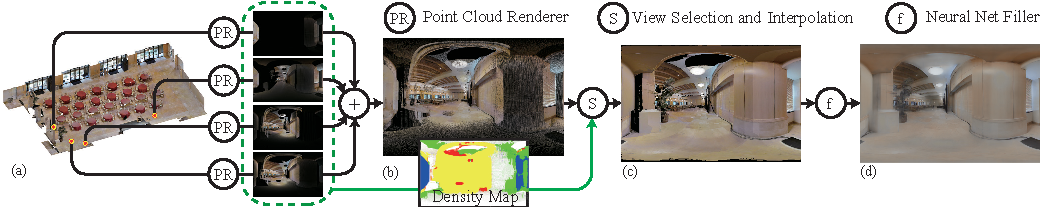
\includegraphics[width=\linewidth]{images/gibson_rendering_pipeline.pdf}
	\caption{The Gibson's rendering pipeline. Image from \cite{gibson}.}
	\label{fig:gibsonrenderingpipeline}
\end{figure}
At first, the given RGB-D panoramas are transformed into point clouds and each pixel is projected from equirectangular coordinates to Cartesian coordinates. For the desired target view $v_j =
(x_j , y_j , z_j , \theta_j, \phi_j, \gamma_j )$, there are chosen the nearest $k$ views in the
scene database, denoted as $v_{j,1}, v_{j,2}, ..., v_{j,k}$. The point cloud of each $v_{j,i}$ coordinate is transformed to $v_j$ coordinate with a rigid body transformation, and the final point cloud is projected onto an equirectangular image (Fig. \ref{fig:gibsonrenderingpipeline}a). Then, the points from all reference panoramas are aggregated to make a single panorama using a locally weighted mixture (Fig. \ref{fig:gibsonrenderingpipeline}b). To do this, the proposed approach calculates the point density for each spatial position (average number of points per pixel) of each panorama. Hence, the points in the aggregated panorama are adaptively selected from all views. Next, the authors perform a bilinear interpolation on the aggregated points of the final panorama
points in one equirectangular image to reduce the empty space between rendered pixels (Fig. \ref{fig:gibsonrenderingpipeline}c). Finally, the method uses a neural network, called $f$ or ``filler'', to fix artifacts and generate a more real-looking image given the output of geometric point cloud rendering (Fig. \ref{fig:gibsonrenderingpipeline}d). This deep model trains a network for making rendered frames look more like real images (forward function) as well as another network that makes real images look like renderings (backward function). The two functions are trained to produce equal outputs. The backward function resembles deployment-time corrective
glasses for the agent, so the authors call it \textit{Goggles}.

\subsection{Matterport3D}

In \citeyear{matterport}, \citeauthor{matterport} introduced Matterport3D, a large-scale RGB-D dataset of 90 digitizes real environments. The dataset comprises a set of 194,400 RGB-D images captured in 10,800 panoramas from 90 real-world scenes. It includes both depth and color $360^{\circ} $ panoramas for each viewpoint and provides camera poses that are globally consistent and aligned with a textured surface reconstruction. Furthermore, Matterport3D includes instance-level semantic segmentation into region and object categories.

In the Matterport data acquisition process, an operator captures
a set of panoramas uniformly spaced at approximately 2.5m
throughout the entire walkable floor plan of the environment (Fig. \ref{fig:matterport-panoramas}). It uses a camera system rig with three color and three depth cameras pointing slightly up, horizontal, and slightly down. At each panorama (acquisition point), the rig rotates around the direction of gravity to
6 distinct orientations, acquiring an HDR photo from each of the 3 RGB cameras for each orientation. The 3 depth cameras acquire data continuously as the rig rotates, which is integrated to synthesize a 1280x1024 depth image aligned
with each color image. The result for each panorama is 18 RGB-D images. 

\begin{figure}[h!]
	\centering
	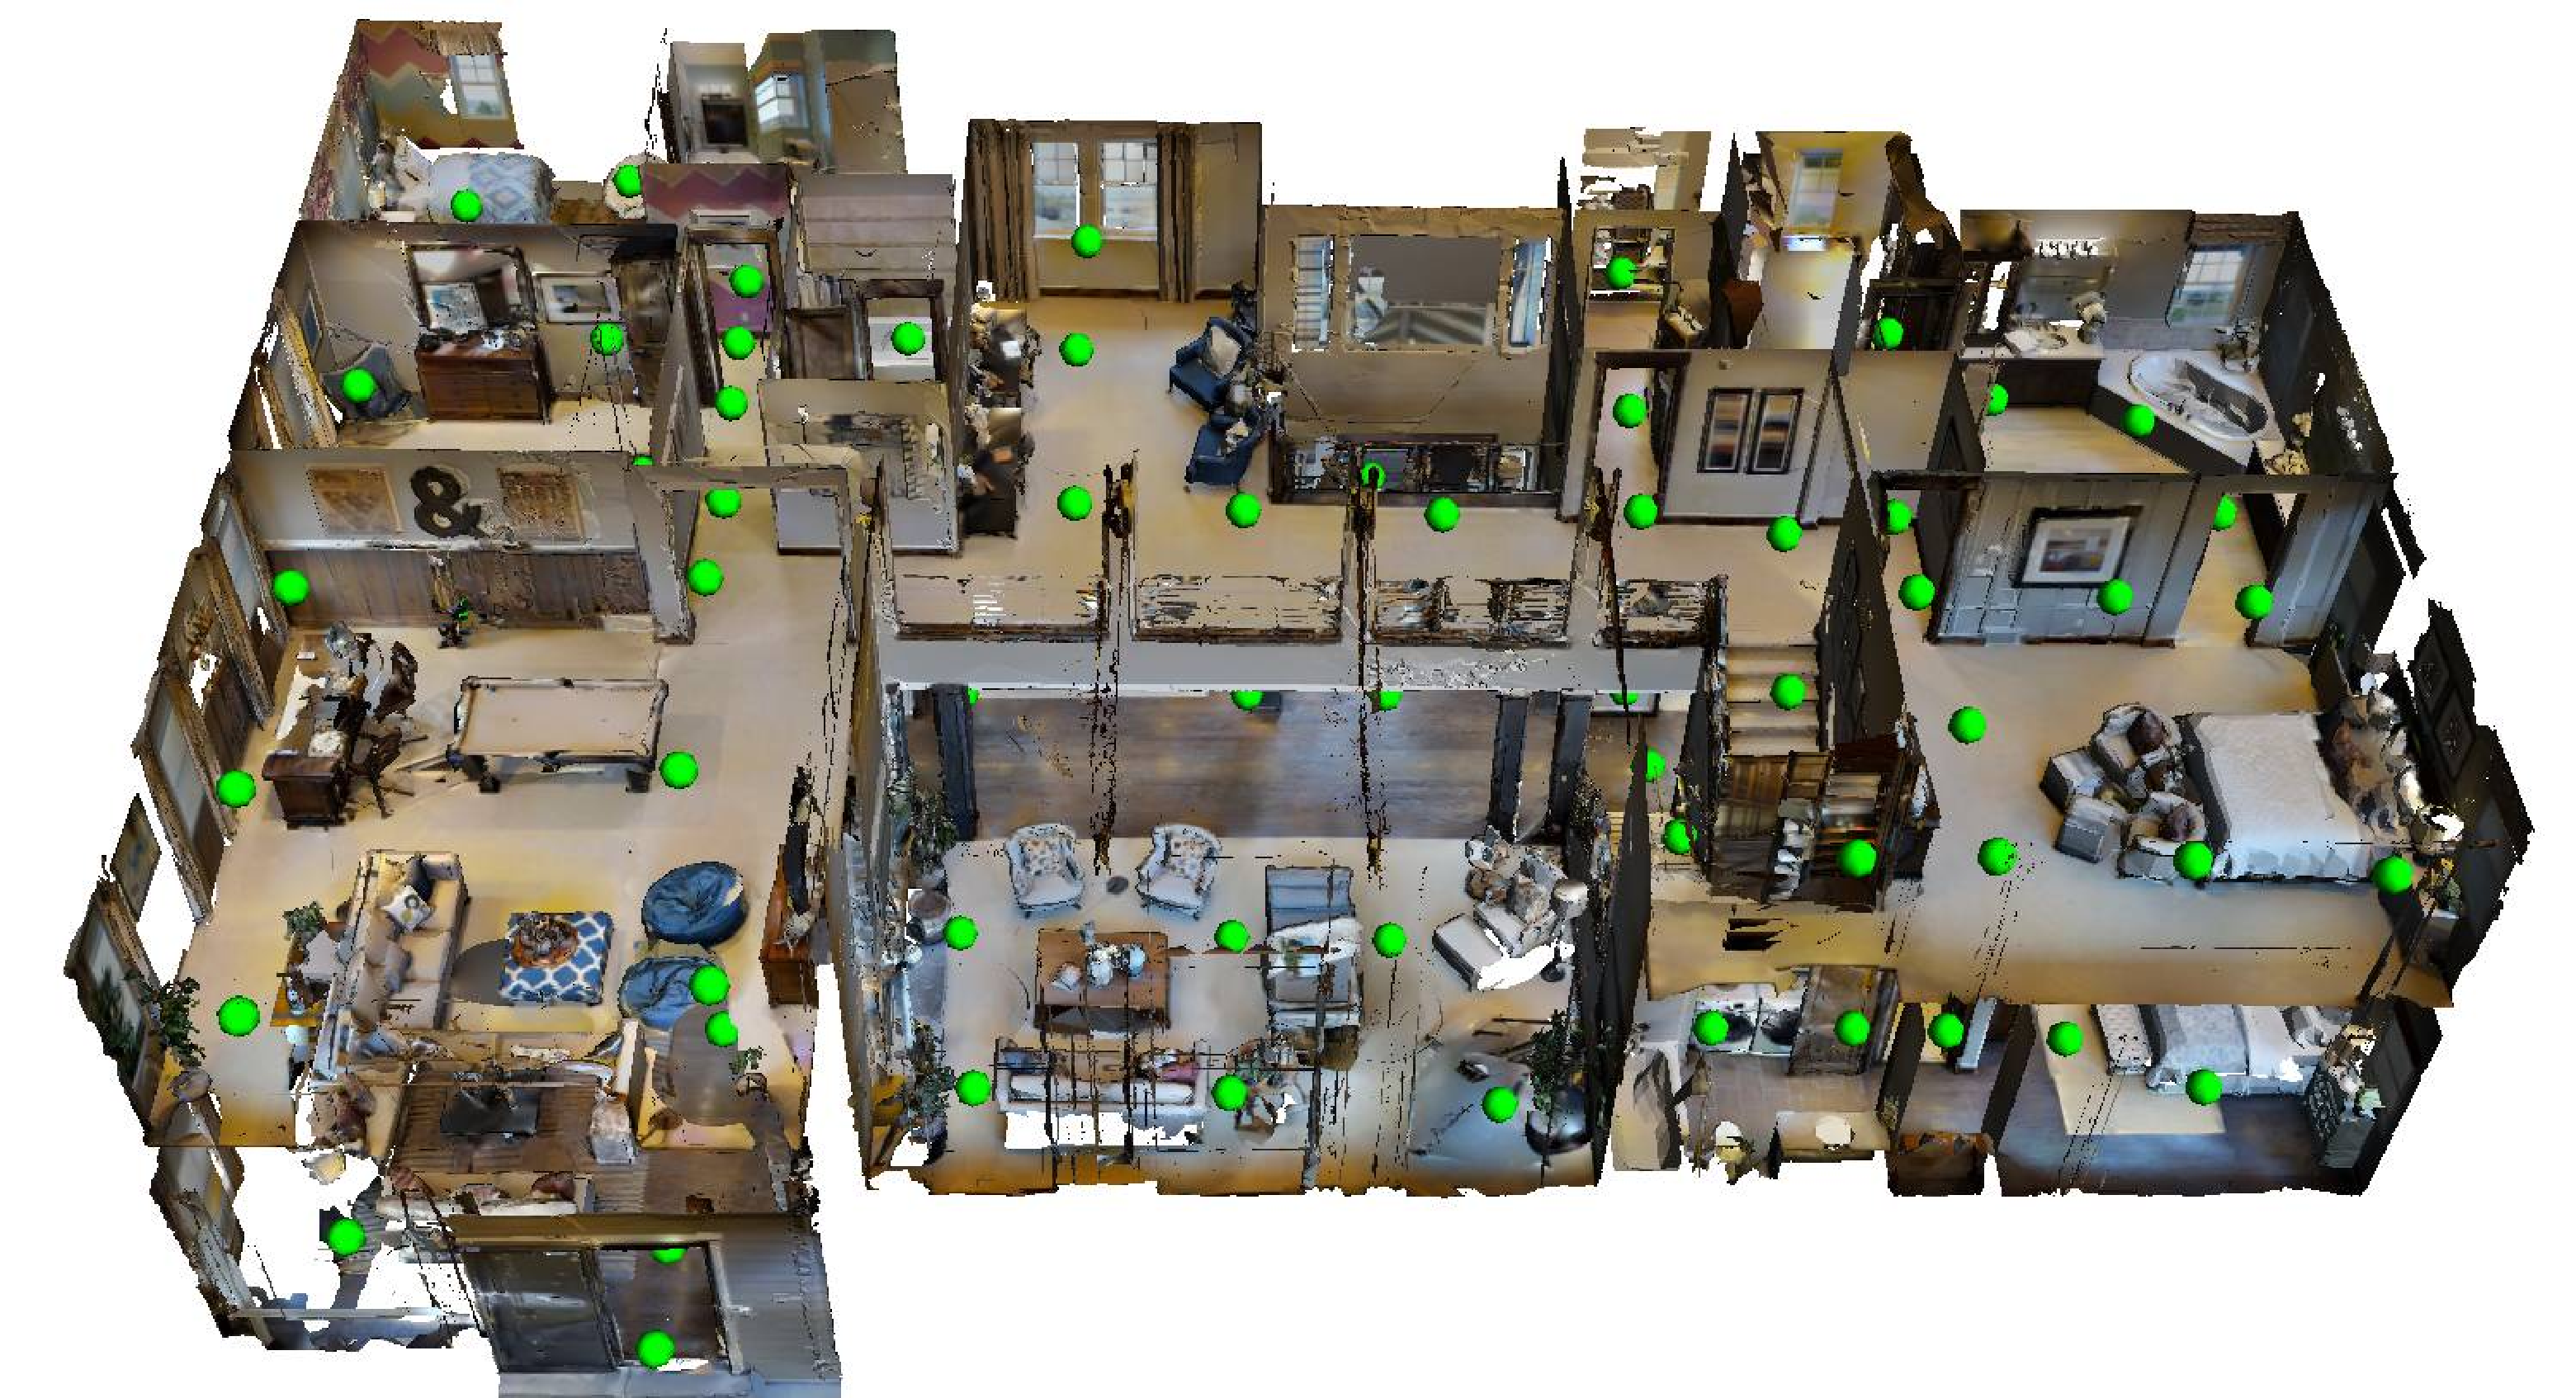
\includegraphics[width=\textwidth]{images/panoramas.pdf}
	\caption{The viewpoints from which panoramas are captured. Image from \cite{matterport}.}
	\label{fig:matterport-panoramas}
\end{figure}

The authors also provide instance-level semantic annotations in 3D. The first step of the annotation process is to break down each building into region components by specifying the 3D spatial extent and semantic category label for
each room-like region. This is done using a simple interactive tool in which the annotator draws a 2D polygon on the floor plans for each region (Fig. \ref{fig:matterport-floor-annotation}). The second step provides an instance and a category level segmentation on objects in each region. Given a 3D mesh of region (Fig. \ref{fig:matterport_object_annotation_1}), the first type of segmentation (instance-level) assigns a different label for each object instance (Fig. \ref{fig:matterport_object_annotation_2}) while the latter (category-level) associates different labels for different object types (Fig. \ref{fig:matterport_object_annotation_3}). To do that, the authors extract a mesh for each region and process it with the crowd-source interface of ScanNet  proposed by \citeauthor{scannet} \cite{scannet}. Using the open-source code provided with ScanNet, the authors of Matterport3D perform surface reconstruction of regions' meshes to ``paint'' triangles to segment and name all object instances
within each region. The 3D segmentations contain a total of 50,811 object
instance annotations divided into 40 objects categories.

\begin{figure}[h!]
	\centering
	\begin{subfigure}[b]{\linewidth}
		\centering
		\begin{subfigure}[b]{0.48\linewidth}
			\centering
			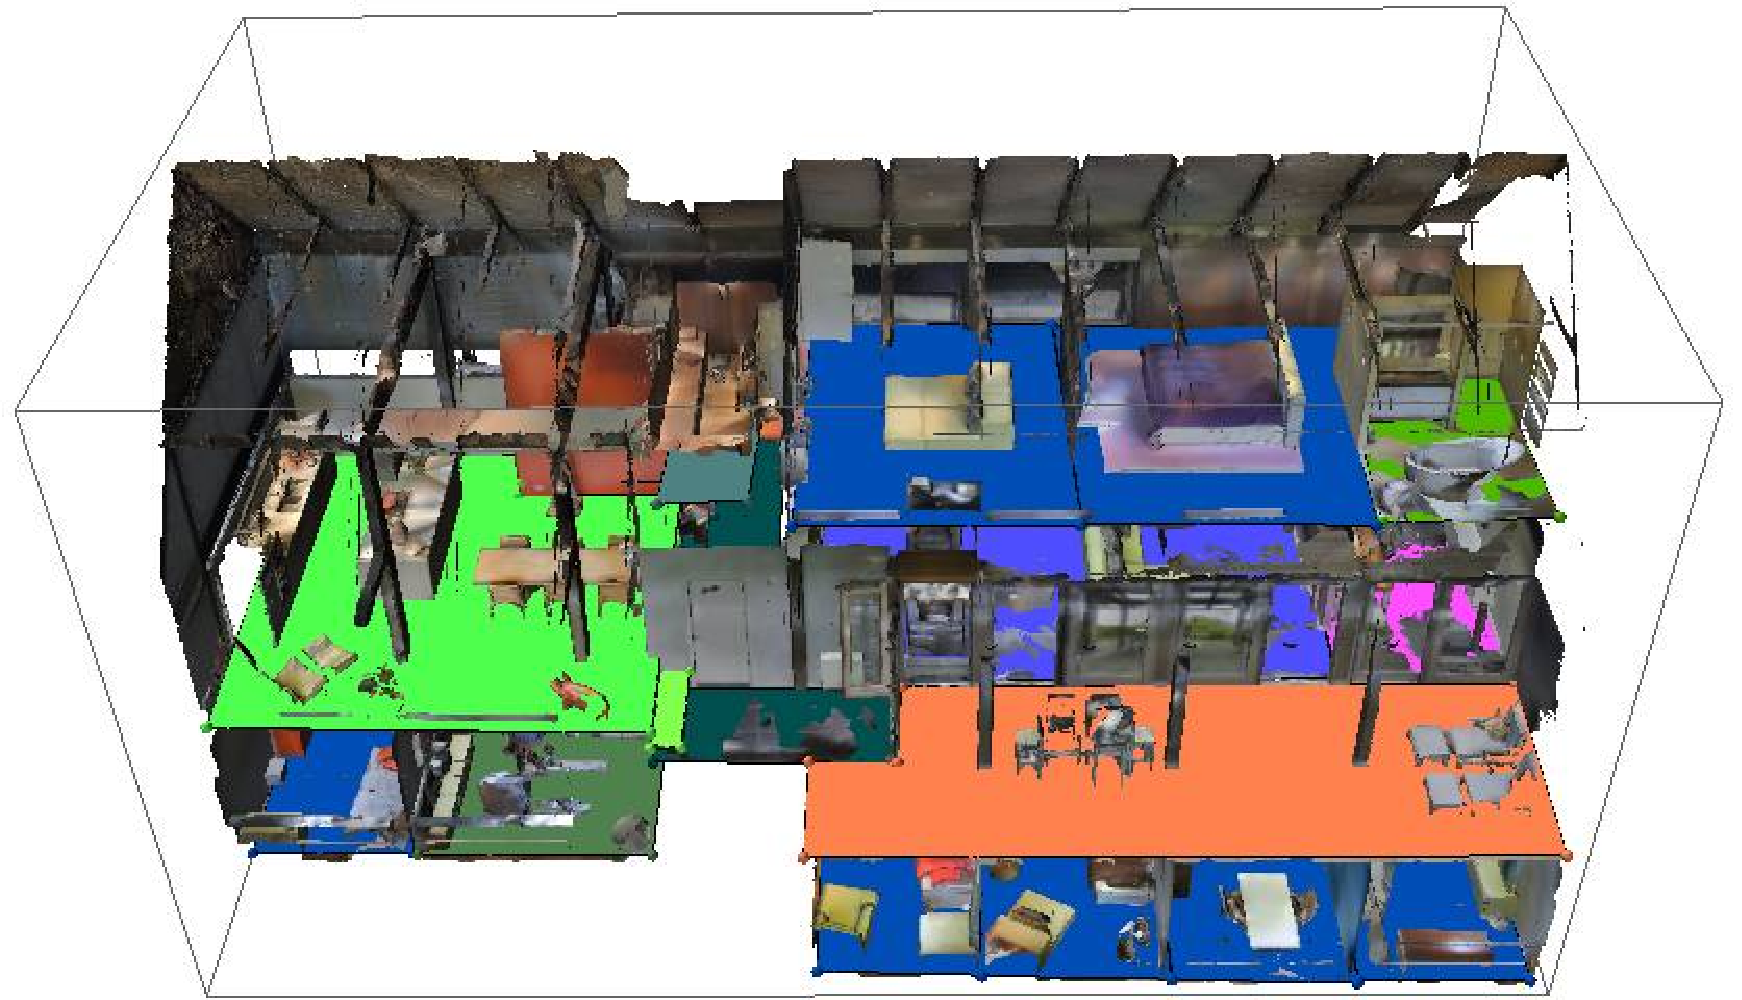
\includegraphics[width=\textwidth]{images/matterport_surfaces_by_label.pdf}
		\end{subfigure}
		\hfil
		\begin{subfigure}[b]{0.48\linewidth}
			\centering
			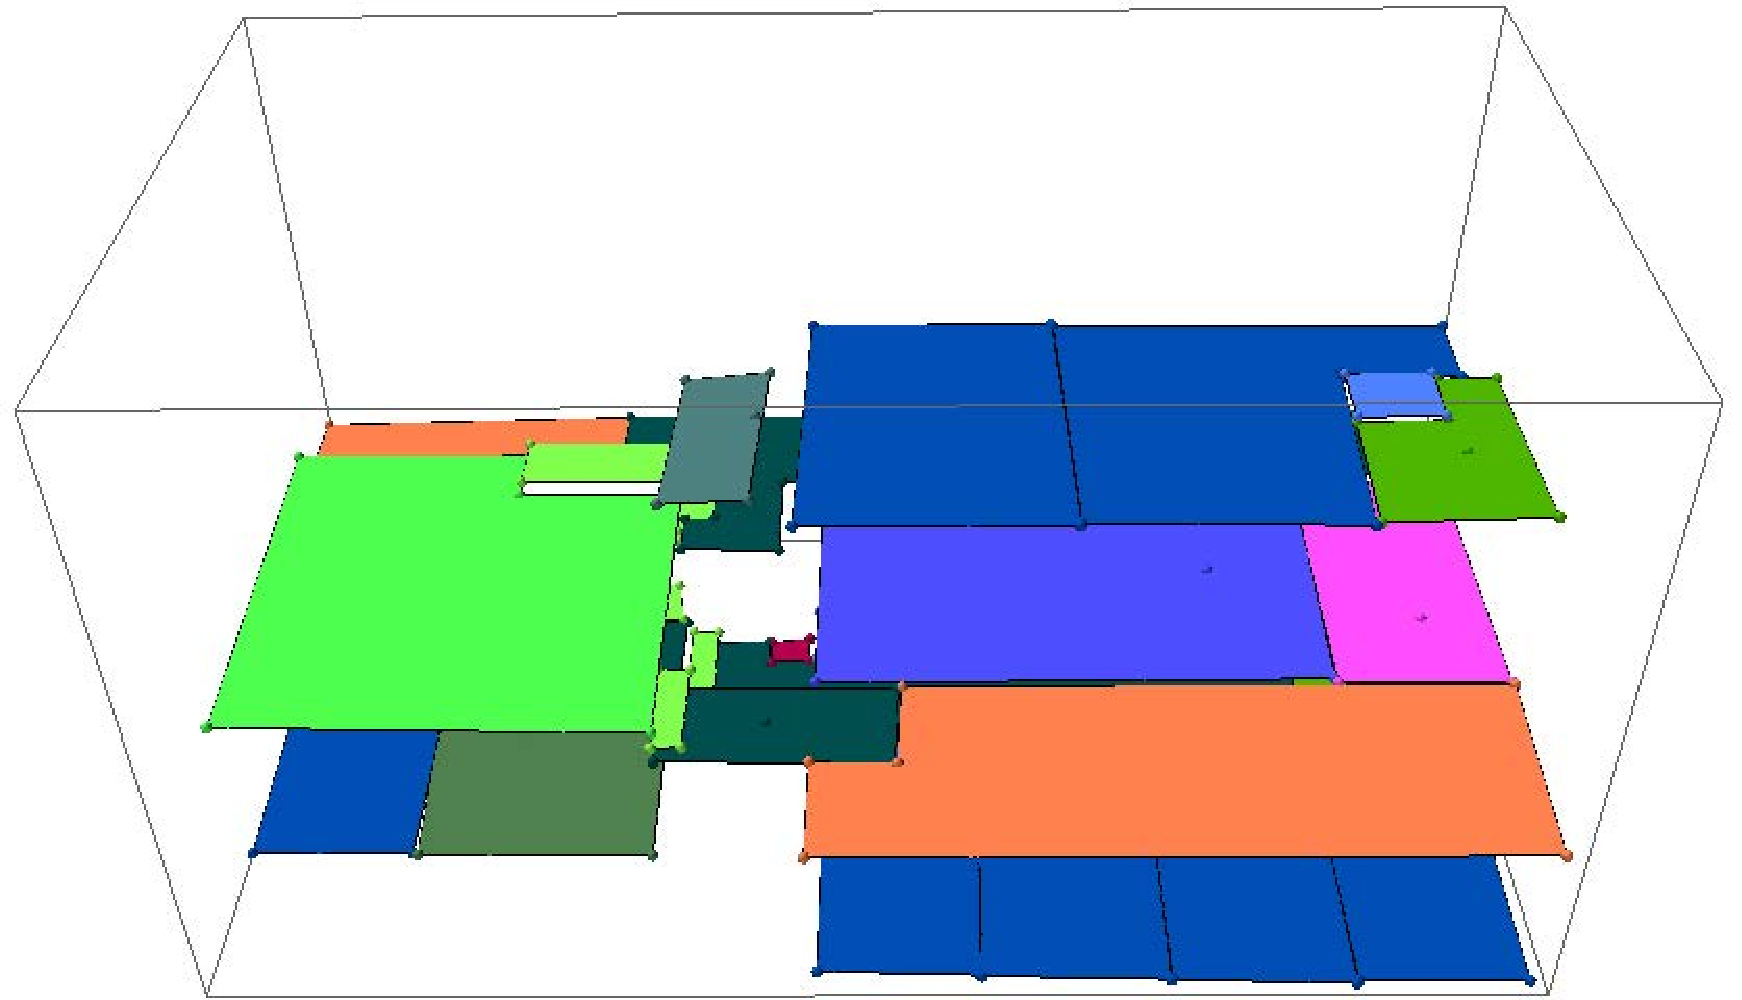
\includegraphics[width=\textwidth]{images/surfaces_by_label.pdf}
			
		\end{subfigure}
	\caption{}
	\label{fig:matterport-floor-annotation}
	\end{subfigure}
	\newline
	\begin{subfigure}[b]{\linewidth}
		\centering
		\begin{subfigure}[b]{0.32\linewidth}
			\centering
			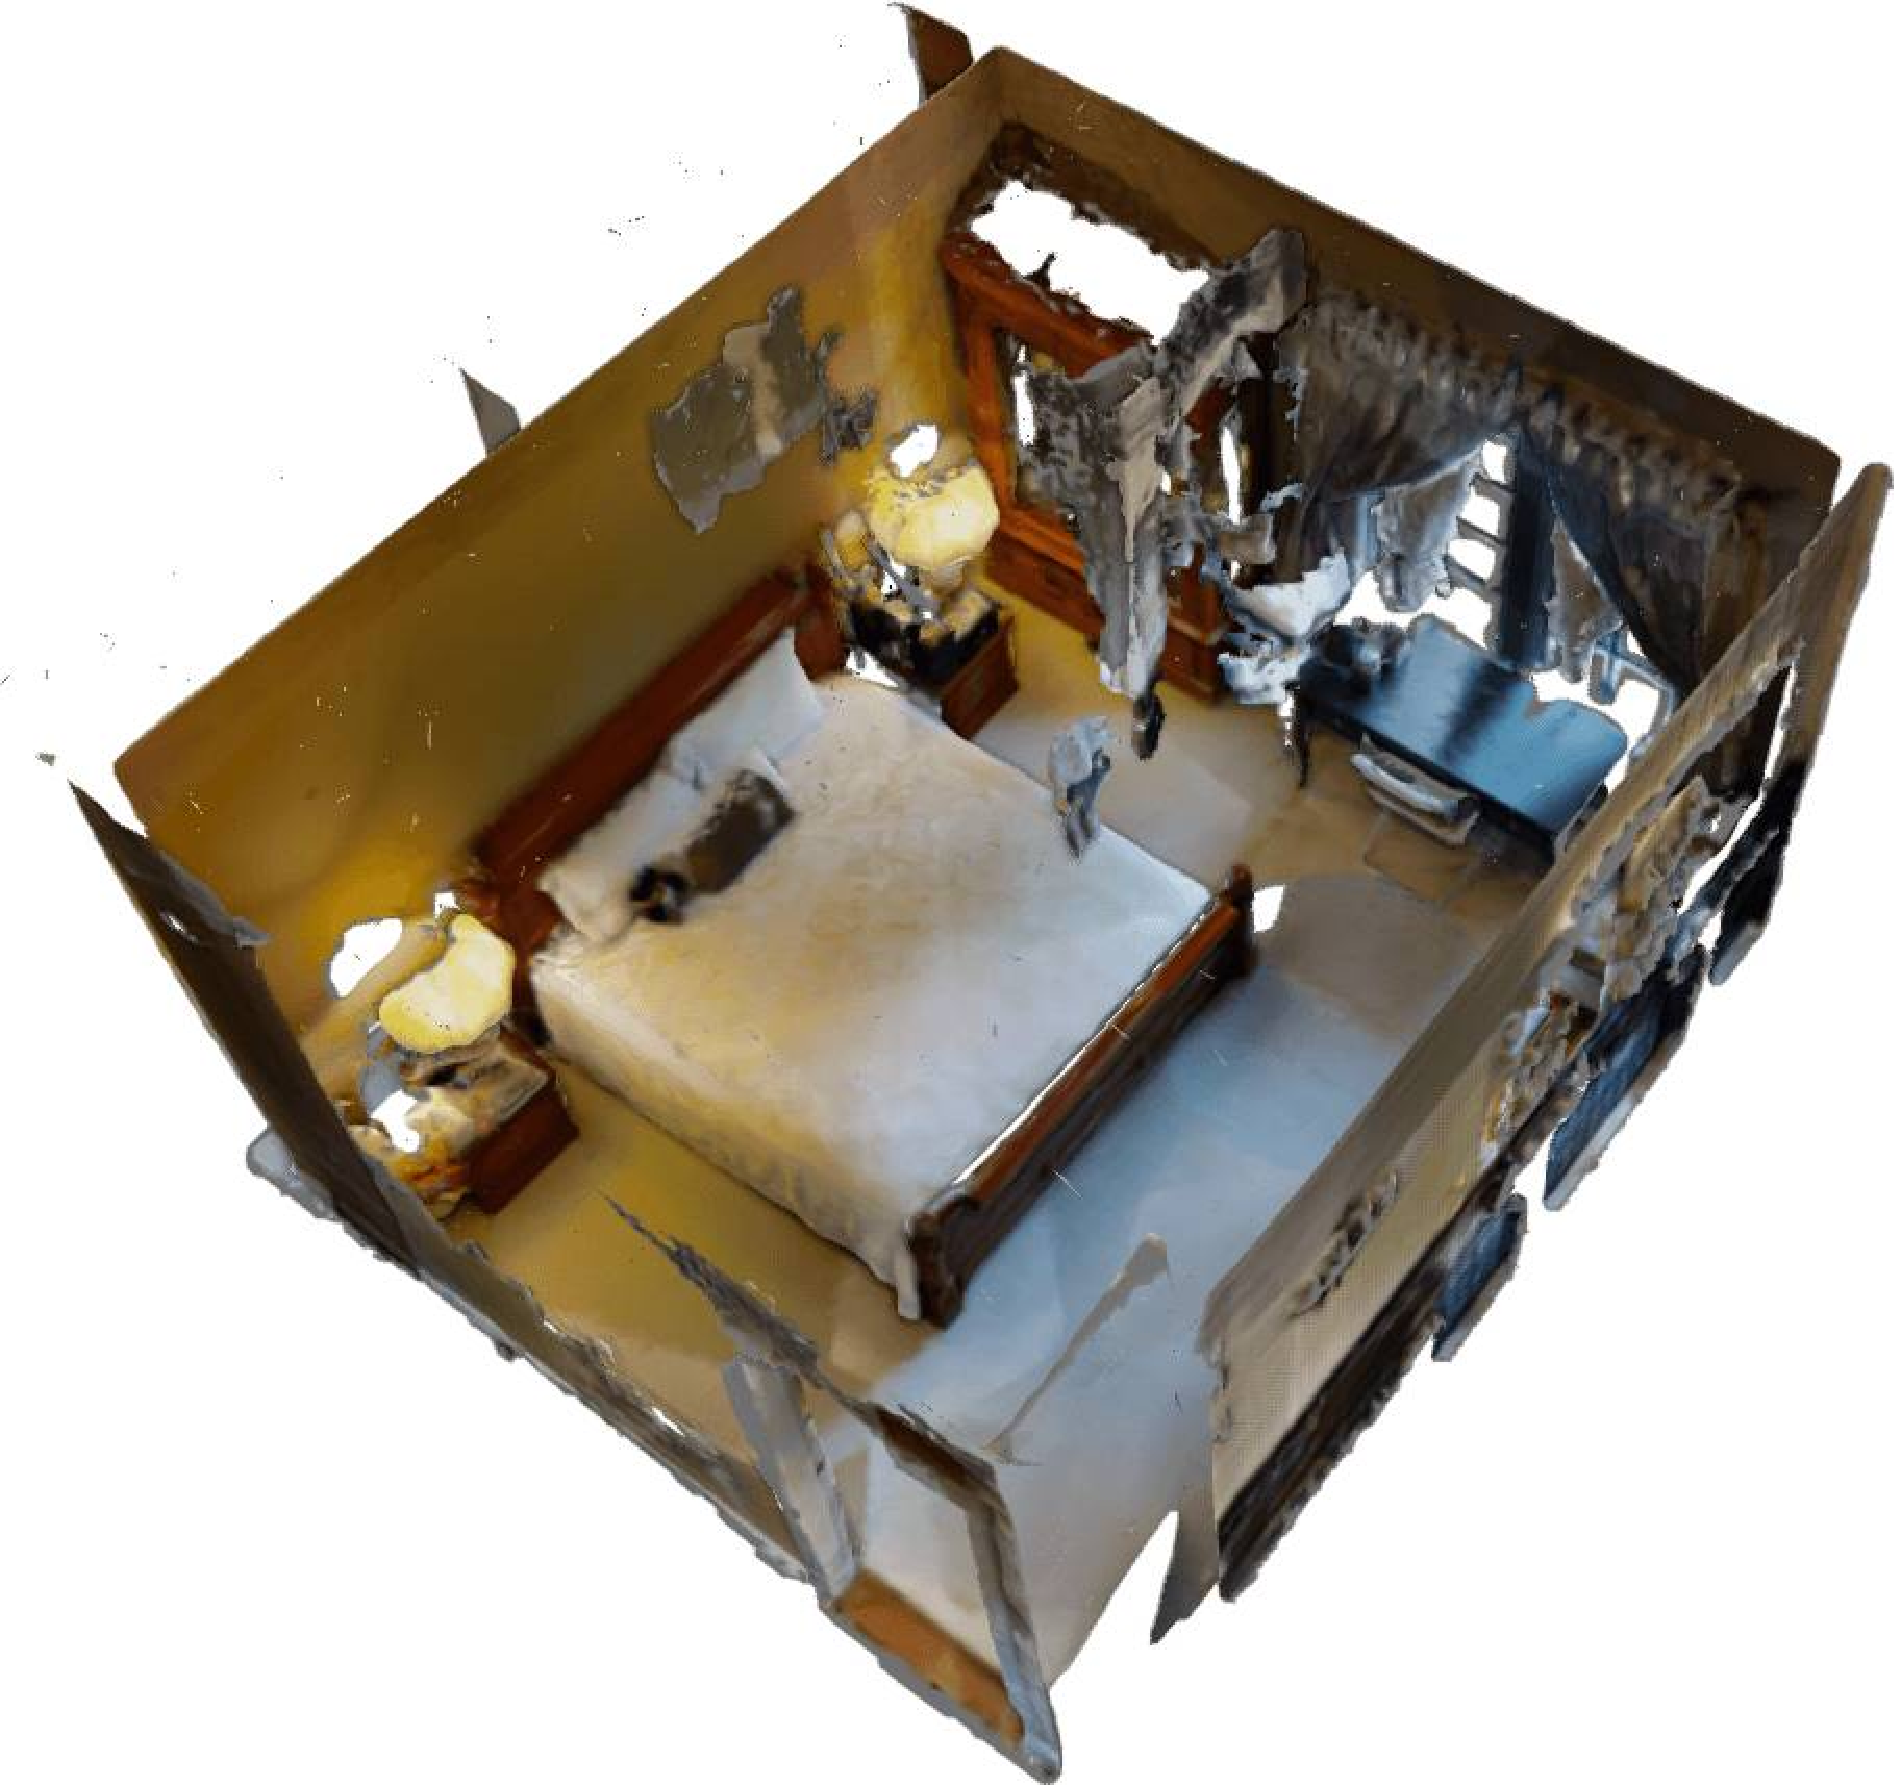
\includegraphics[width=\textwidth]{images/matterport_room22_color.pdf}
			\caption{}
			\label{fig:matterport_object_annotation_1}
		\end{subfigure}
		\hfil
		\begin{subfigure}[b]{0.32\linewidth}
			\centering
			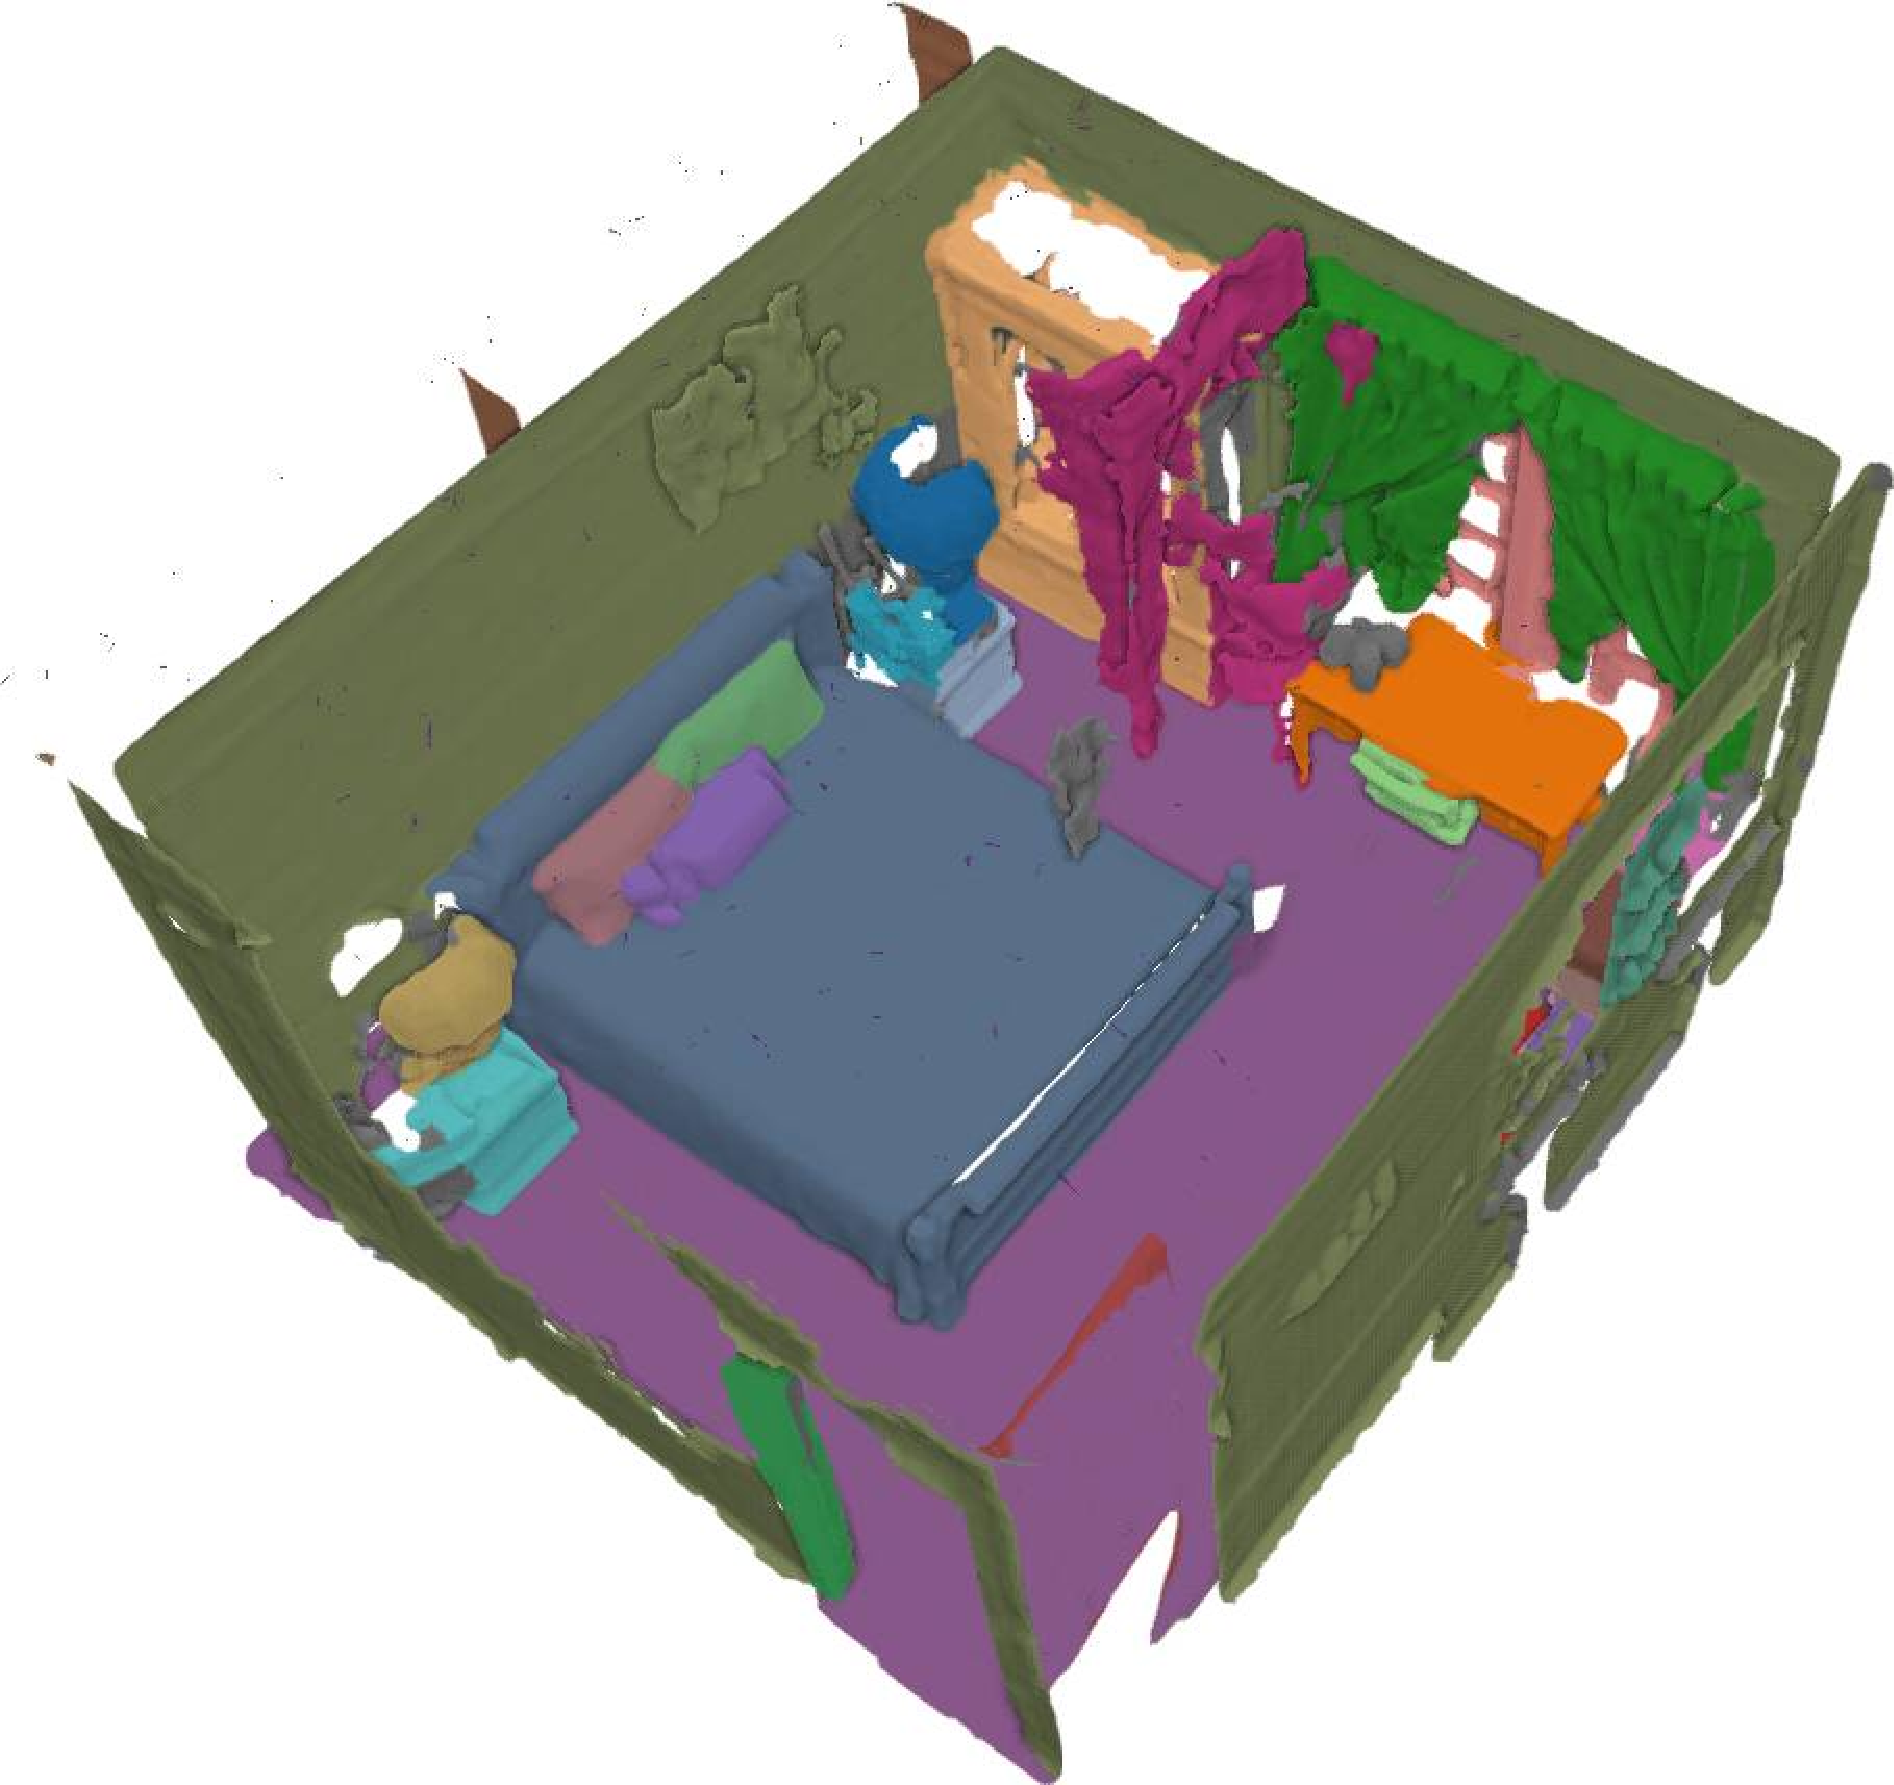
\includegraphics[width=\textwidth]{images/matterport_room22_instances.pdf}
			\caption{}
			\label{fig:matterport_object_annotation_2}
		\end{subfigure}
		\hfil
		\begin{subfigure}[b]{0.32\linewidth}
			\centering
			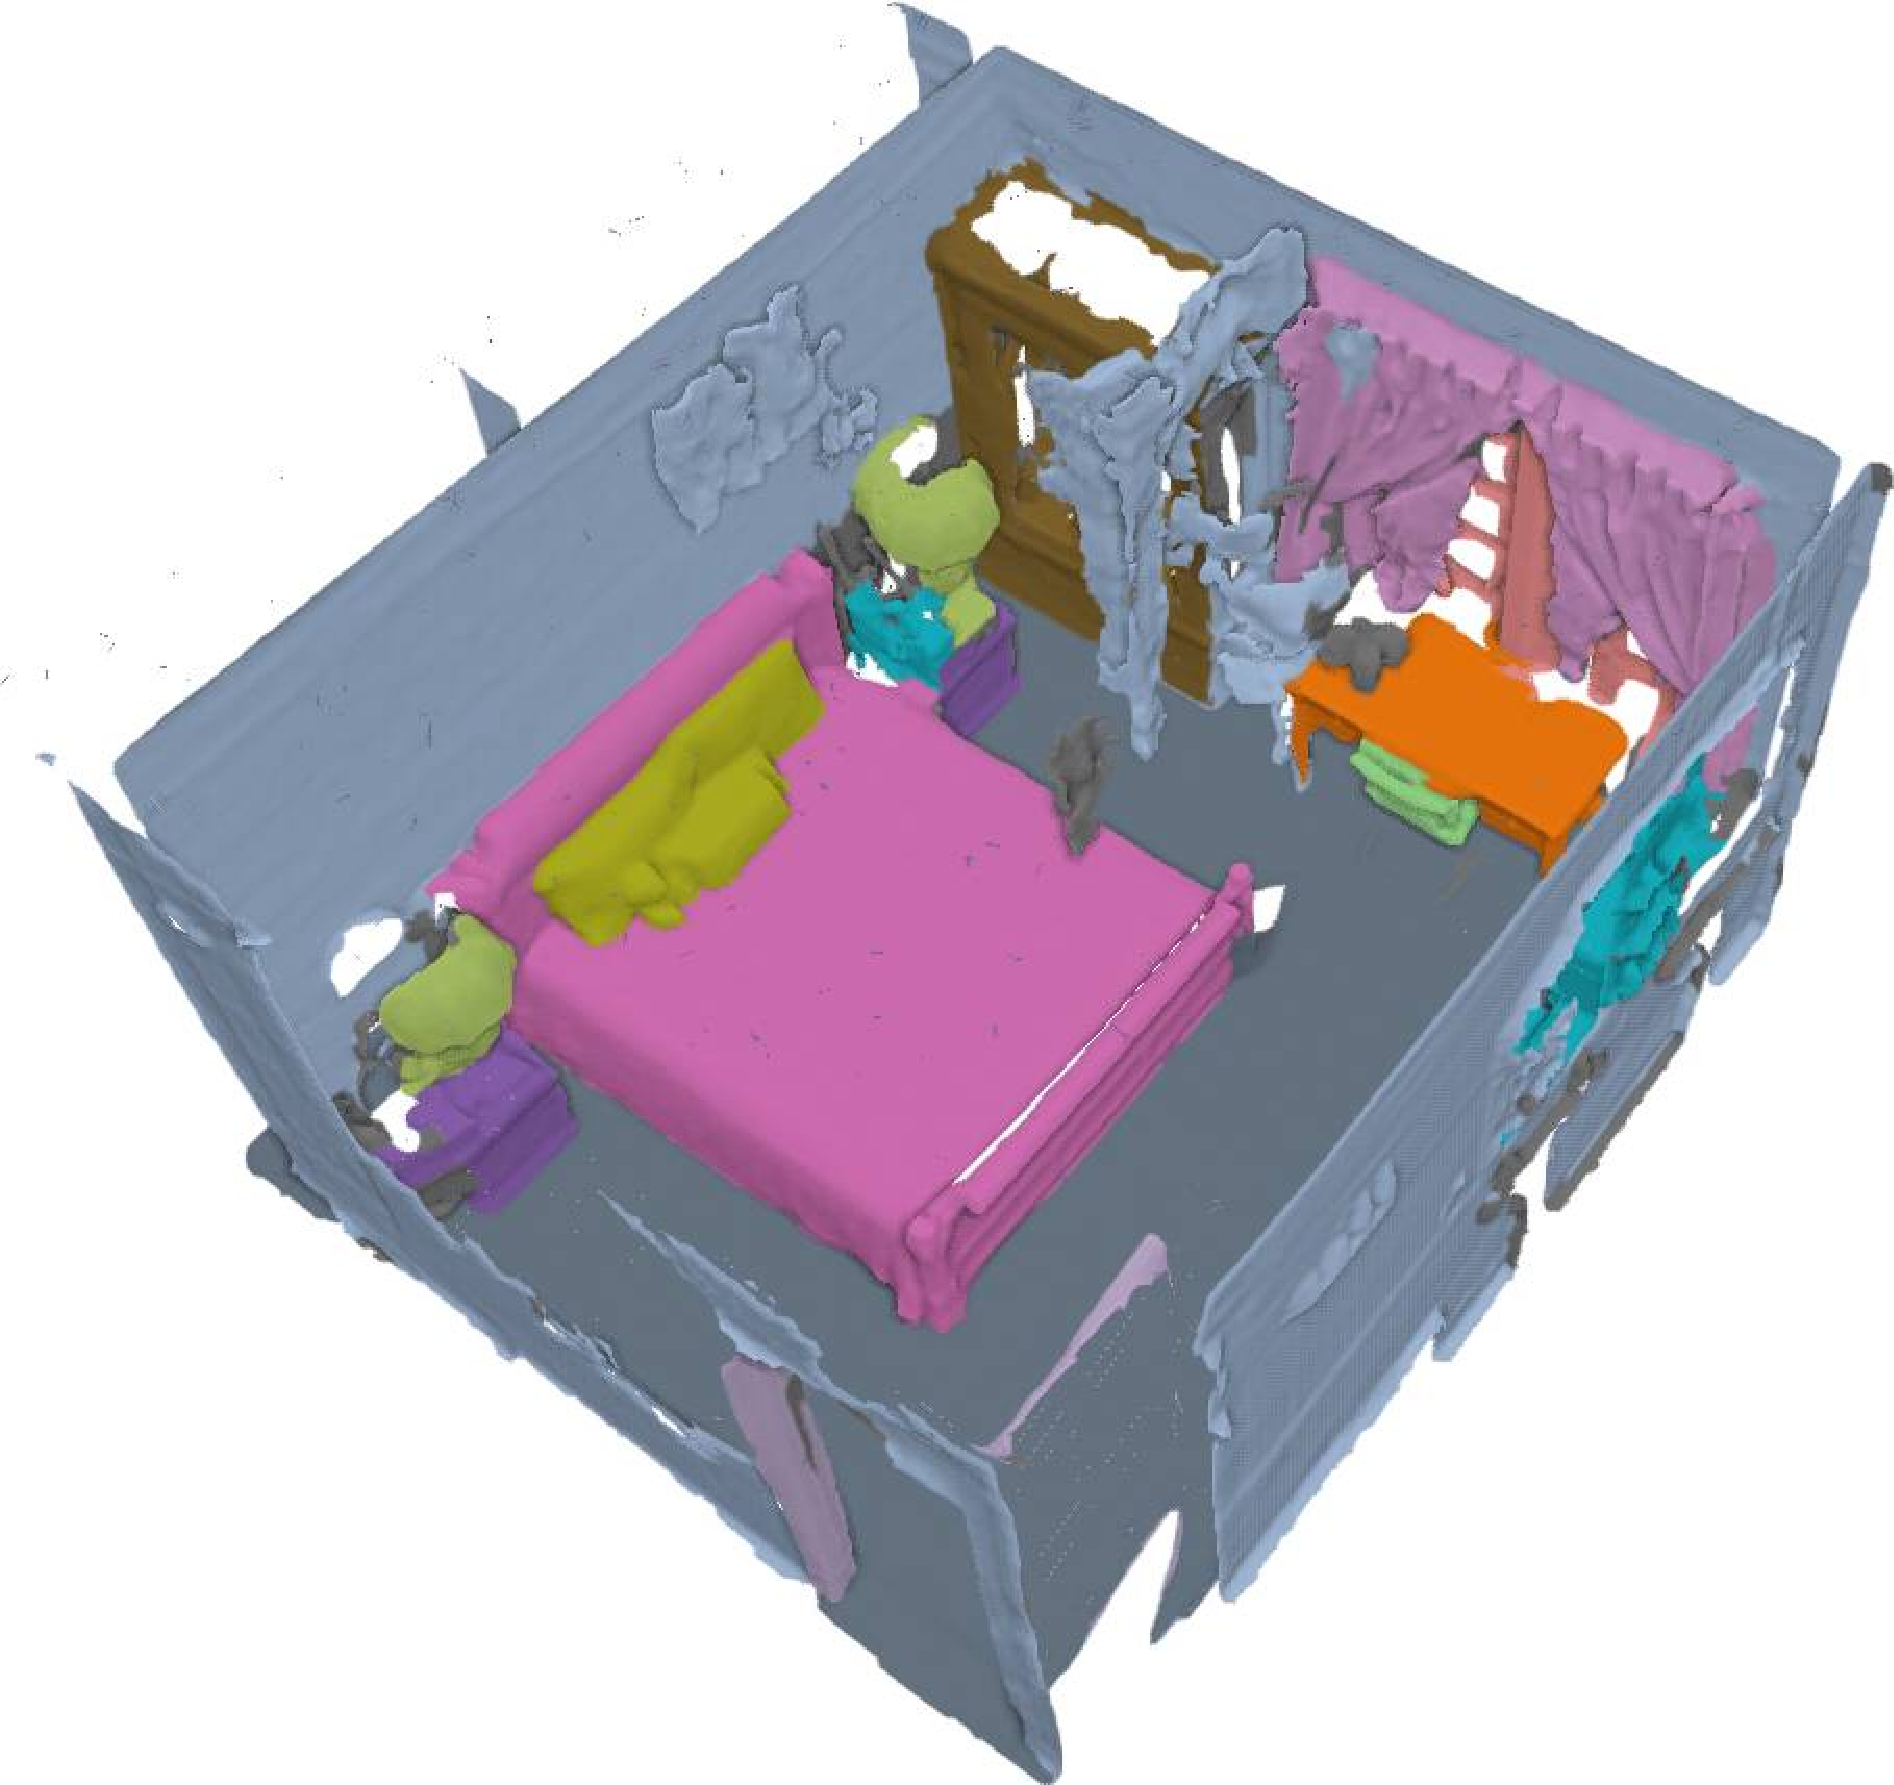
\includegraphics[width=\textwidth]{images/matterport_room22_categories.pdf}
			\caption{}
			\label{fig:matterport_object_annotation_3}
		\end{subfigure}
	\end{subfigure}
	\caption{(a) Region annotation on floor plans. (b, c, d) Instance and category object segmentation of floor plan's region. Images from \cite{matterport}.}
\end{figure}

\subsection{New Gibson Version}
\label{sec:new_gibson_version}

Gibson and Matterport3D are the selected packages to acquire the dataset to train and evaluate the proposed robotic doors detector. In the first experiments, we argue that these technologies present some problems and limitations that affect an easy and fast data collection procedure. 

A suitable way for acquiring a visual robotic dataset in simulation is to embodies a virtual agent which autonomously explores a simulated environment using the standard navigation stack. In this way, the examples captured during its navigation are coherent with a real exploration strategy, reflecting how a real robot perceives an indoor scene. Unfortunately, this solution is infeasible with the selected technologies. 

First of all, this technique is extremely time-consuming. Gibson perfectly simulates the real features of mobile agents (e.g. the speed of movement, the sensors' accuracy, and the physical characteristics). This fact allows us to use the standard navigation stack that is generally provided for well-known mobile robots (e.g. Turtlebot2 \cite{turtlebot2}, Turtlebot3 \cite{turtlebot3}, or Husky car \cite{husky}). Despite this, the real-time simulation provided by Gibson makes the data acquisition extremely slow, especially for large environments.  Furthermore, the dataset would be suitable for multiple robots with different navigation packages and camera heights. This fact implies performing multiple runs in the same environments with different agents, further extending the acquisition time. Due to navigation is a challenging task, an autonomous agent can crash into an obstacle or iterate the same actions due to a software issue. In simulated environments, fixing robot failures is often infeasible, making the runs useless. 

Another issue is related to the exploration, which can be performed through different strategies (such as frontier-based exploration \cite{frontierexploration}) that do not guarantee the experiments' repeatability. In different runs, the robot can follow different paths and the exploration time can vary a lot. In this way, the dataset is heavily dependent on the chosen exploration strategy.

While the issues just reported can be solved using appropriate techniques, the problem related to the Matterport3D dataset makes completely infeasible data collection using Gibson ``as is''. The physical structure of the Matterport's environments is encoded in 3D polygonal meshes. A polygon mesh is a collection of vertices, edges, and faces that defines the shape of a polyhedral object. These meshes are extremely cluttered and noisy. The furniture models are malformed and incomplete, e.g. a table can be composed of the horizontal plan omitting one or more legs (Fig. \ref{fig:matterport_issues_meshes_furniture}), or some faces are disconnected from the principal object mesh. Furthermore, the walls often present holes at windows, mirrors, or other undefined locations (Fig. \ref{fig:matterport_issues_hole}). These malformations affect the robot perception, making autonomous navigation impossible. Another important aspect concerns the floor plans' surfaces, that are extremely irregular. They are composed of a series of triangles but the vertexes are not perfectly aligned (Fig. \ref{fig:matterport_issues_floor_plan}). This further complicates the robot navigation, which often crashes over floor irregularities.

\begin{figure}[h!]
	\centering
	\begin{subfigure}[b]{0.32\linewidth}
		\centering
		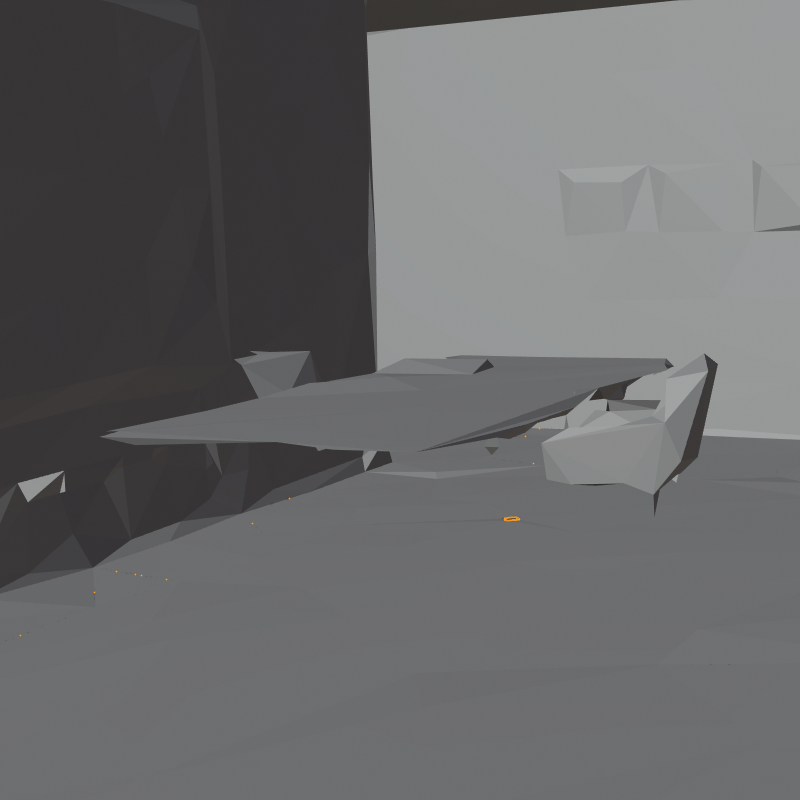
\includegraphics[width=\textwidth]{images/table.png}
		\caption{}
		\label{fig:matterport_issues_meshes_furniture}
	\end{subfigure}
	\hfil
	\begin{subfigure}[b]{0.32\linewidth}
		\centering
		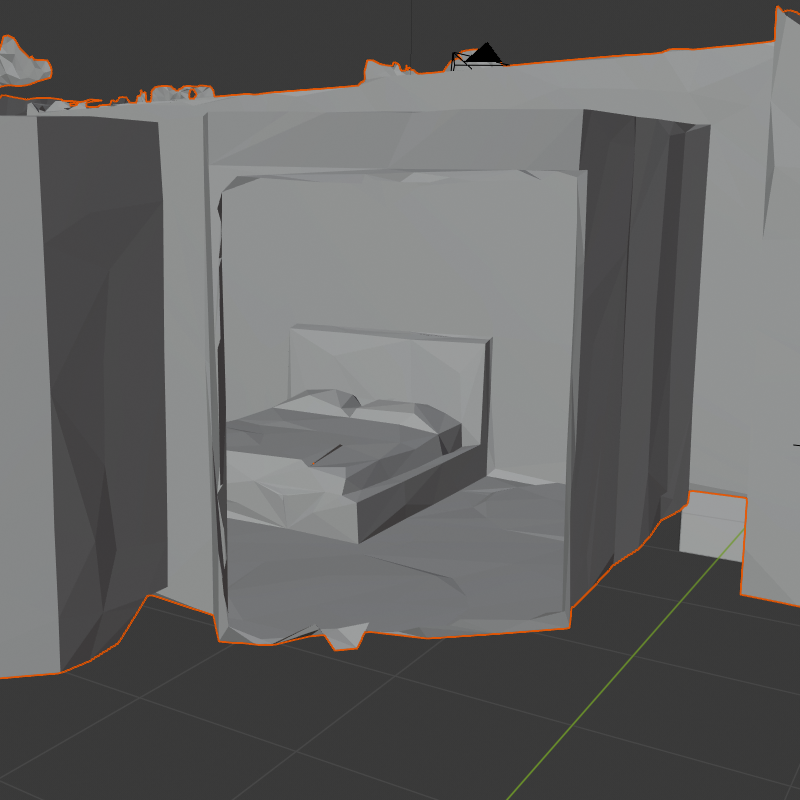
\includegraphics[width=\textwidth]{images/holes.png}
		\caption{}
		\label{fig:matterport_issues_hole}
	\end{subfigure}
	\hfil
	\begin{subfigure}[b]{0.32\linewidth}
		\centering
		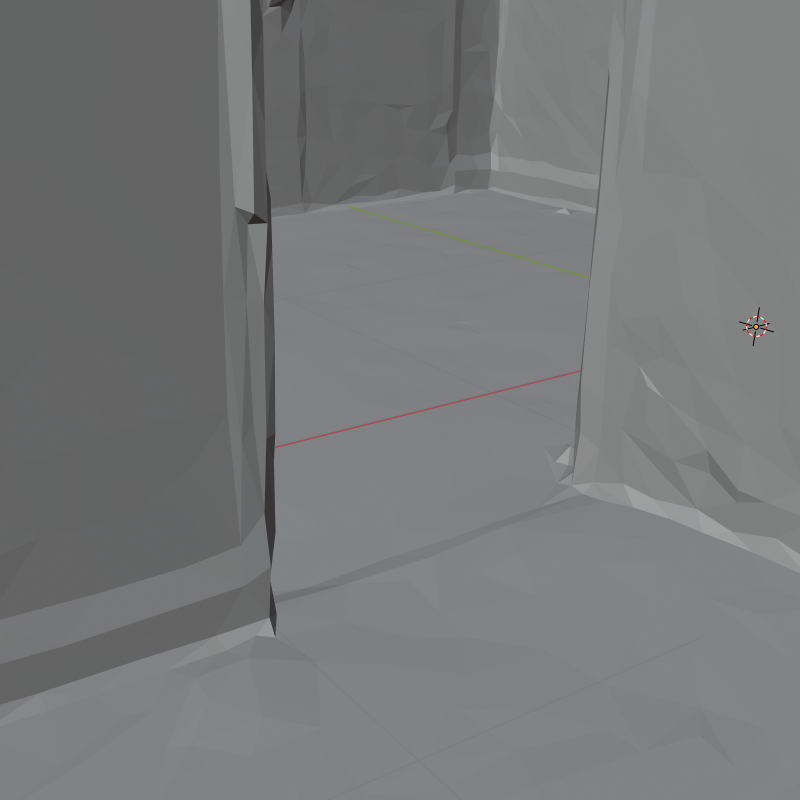
\includegraphics[width=\textwidth]{images/floor_plan_irregularity.png}
		\caption{}
		\label{fig:matterport_issues_floor_plan}
	\end{subfigure}
	\caption{Matterport3D mesh malformations. (a) A suspended table and chair. (b) A holes in a bedroom. (c) Floor plan irregularities.}
\end{figure}


To overcome these difficulties, we provide an upgraded version of Gibson available on Github\footnote{The code of the new Gibson version: \url{https://github.com/micheleantonazzi/GibsonEnv}.}. We developed a new simulation mechanism without any physical constraints: gravity and collision detection are removed. Inside this stage, the robot can not move autonomously using motors, but the user can set an absolute position and orientation in which the robot must be located at each instant. In other words, we implement an unreal simulation mechanism in which a robot can both instantly teleport in any location and traverse obstacles. In this way, the user can perform data acquisition in batch without any failure. The robot does not crash over the floor's irregularities, does not go out of the mesh, and can autonomously traverse multiple floors without dealing with architectural barriers (such as stairs or elevators).

The new version of Gibson we released implements further improvements. First of all, we resolve some building errors (that occurs especially in Ubuntu 20.04), and automatize the compile procedure, implementing it inside the \textsf{setup.py} file. In this way, with the simple command \textsf{pip install gibson}, the simulation environment is compiled and installed. The necessary dependencies have been added as Git sub-modules. In this way, they are automatically downloaded and compiled, simplifying the dependencies management. Then, we developed a new and more efficient module to manage Gibson's assets, such as the neural network's weights, the virtualized agents, or the worlds dataset. We also offer a command-line interface to automatically download and extract the assets files from the links provided by the authors. To use it, the user can type three different commands (after Gibson's installation) in a console terminal: \textsf{gibson-set-assets-path} for specifying the assets' folder, \textsf{gibson-download-dataset} to download the provided worlds dataset, and \textsf{gibson-download-assets-core} to retrieve the remaining assets files. Finally, we provide a compiled version of Gibson available on PyPI\footnote{The compiled version of Gibson: \url{https://pypi.org/project/gibson/}.} following the manylinux standard\footnote{The manylinux repository: \url{https://github.com/pypa/manylinux}.}. We offers also a utility package, called \textit{gibson-env-utilities}\footnote{The gibson-env-utilities source code: \url{https://github.com/micheleantonazzi/gibson-env-utilities}.}, to facilitate the usage of Gibson. It automatizes the launch of simulation runs, by offering a class that automatically creates the Gibson configuration file in which the run parameters are specified. Furthermore, \textit{gibson-env-utilities} provides a mechanism to store and retrieve the metadata related to Gibson's scenes. This metadata includes the environment name, the belonging dataset (Matterport3D \cite{matterport} or Stanford-2D-3D \cite{stanford2d3d}) a boolean value that indicates if the environment is semantically annotated, and the number of floors. In addition, for each floor is provided the floor's height and a valid position on such a floor in which the robot can be placed.


\section{Pose Estimator}
\label{sec:pose_estimator}
Thanks to our new simulation stage integrated into the new version of Gibson (described in Sec. \ref{sec:new_gibson_version}), a virtual autonomous agent can be freely positioned and oriented in any environment location. Despite this, to acquire a vision dataset, we need to determine the valid positions in which the robot can be placed: it must be in free space inside the building perimeter, not overlapping obstacles (walls, floors, or furniture). Furthermore, the dataset is used in a robotic vision application, so the samples must be collected in locations consistent with a possible exploration strategy followed by a mobile agent. Typically, a robot walks away from obstacles and chooses the shortest path for moving between different areas. To address these requirements, we developed a method called Pose Estimator, which is based on the work proposed by \citeauthor{repeatabilityslamarxiv} in \cite{repeatabilityslamarxiv, repeatabilityslam}.

Pose Estimator is the component that extracts plausible positions for an autonomous agent from which collect the dataset. This tool performs the computation of the Voronoi graph over the 2D occupancy grid map \cite{cuupancygridfirst} of a floor plan and chooses the positions by sub-sampling this graph. A Voronoi diagram is a partition of a plane into regions close to a given set of points (also called seeds, sites, or generators). Each Voronoi cell contains all points of the plane closer to that seed than to any others. The following paragraphs describe the procedures performed by this module, which is implemented in the \textit{gibson-env-utilities} package.



\paragraph{Extract the 2D Occupancy Grid} The first step concerns the computation of a 2D occupancy grid map (Fig. \ref{fig:pose_estimator_occupancy_grid}) of a floor starting from a 3D mesh (Fig. \ref{fig:pose_estimator_3dmesh}). Each environment of Matterport3D is modeled by a 3D Wavefront file (with \textit{.obj} extension) that stores the position of each vertex and the faces that compose each polygon. The 3D model of an environment is rendered, using a software like Blender\footnote{The Blender's web page: \url{https://www.blender.org/}.}, to estimate the average height of the points that compose the selected floor plan. Then, the method performs multiple cross-sections of the 3D mesh with parallel planes, starting from a few centimeters over the floor. The 2D cross-sections, that detect obstacles at multiple heights, are aggregated and projected in a 2D image. Finally, this image is manually fixed to fill the shortcomings due to mesh inaccuracies or to remove artifacts produced by the cross-section. In addition, it is particularly important that the user closes all the opened contours in the image. This final 2D image (Fig. \ref{fig:pose_estimator_occupancy_grid}) stores the occupancy grid map of a floor plan, where each pixel represents a sub-portion of the environment and contains the probability that it is occupied by an obstacle. Together with the image map, important metadata are also saved, in order to enable conversion operations between map and simulation coordinates. The metadata includes the map's origin (in pixels) and the scale, which specifies how many meters correspond to a pixel.

These operations are implemented in the \textsf{GibsonAssetsUtilities} class of \textit{gibson-env-utilities} package. In particular, \textsf{load\_obj} method loads the Wavefront file while \textsf{create\_floor\_map} extract the floor map and the relative metadata, saving them to the disk. The mesh file loading and the computation of multiple cross-sections are performed using Trimesh\footnote{The Trimesh source code: \url{https://github.com/mikedh/trimesh}.}, a pure Python library for loading and elaborating triangular meshes. The final image is rendered using Matplotlib\footnote{The Matplotlib web site: \url{https://matplotlib.org/}.}, a comprehensive library for creating static, animated, and interactive visualizations in Python. 

\begin{figure}[h!]
	\centering
	\begin{subfigure}[b]{0.49\linewidth}
		\centering
		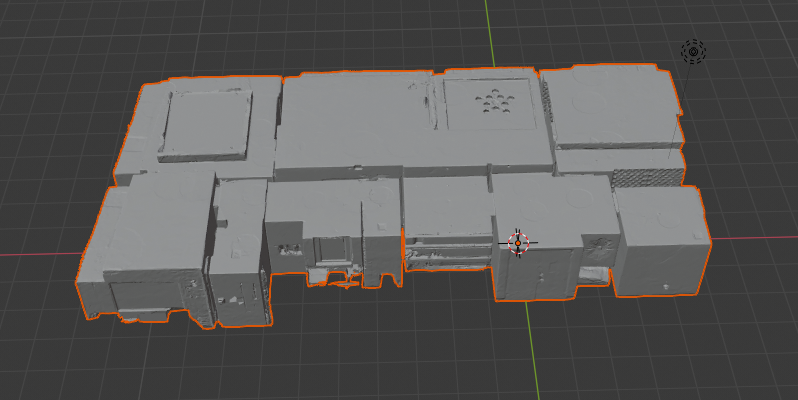
\includegraphics[width=\textwidth]{images/pose_estimator_3Dmesh.png}
		\caption{}
		\label{fig:pose_estimator_3dmesh}
	\end{subfigure}
	\hfil
	\begin{subfigure}[b]{0.49\linewidth}
		\centering
		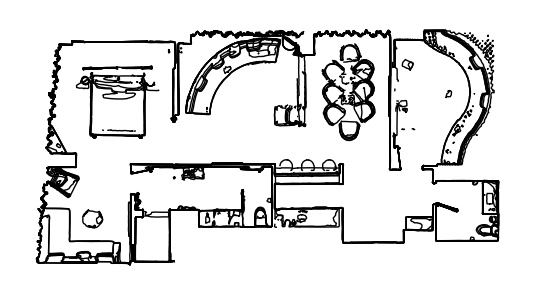
\includegraphics[width=\textwidth]{images/pose_estimator_1.png}
		\caption{}
		\label{fig:pose_estimator_occupancy_grid}
	\end{subfigure}
	\caption{The computation of the 2D occupancy grid map (right) from the 3D mesh (left) of an environment.}
\end{figure}

\paragraph{Compute the Voronoi Bitmap} This step aims to extract the Voronoi bitmap graph from the 2D occupancy grid of a floor (Fig. \ref{fig:pose_estimator_1}). In order to do this, Pose Estimator processes the occupancy grid map, stored in a \textsf{png} image, using OpenCV\footnote{The OpenCV home page \url{https://opencv.org/}.}: a library of programming functions mainly aimed at real-time computer vision. At first, the image is thresholded to obtain a more uniform mask which indicates the free and occupied location. To do this, the module uses the OpenCV's \textsf{threshold} method, which suppresses (leads to zero) all pixels with a color value less than 250. Then, this optimized occupancy grid is eroded and dilated (through the \textsf{erode} and \textsf{dilate} methods of OpenCV) using a $3 \times 3$ kernel to reduce the noise. Now, the method finds the contours (using the OpenCV \textsf{findContours} method) in the smoothed image to identify the boundaries in which the robot can move. The methods return all the contours in the image without any approximation organized in a tree structure, thanks to the \textsf{CHAIN\_APPROX\_NONE} and \textsf{RETR\_TREE} flags respectively. The longest contour is assumed to be the floor's perimeter. The area outside the floor's outline and all its internal contours (that represent the furniture) are black-filled: the resulting image (Fig. \ref{fig:pose_estimator_filled}) highlights in white the free area in which the robot can move. Now, the Voronoi diagram is calculated using the Delaunay triangulation \cite{delaunayproof} (implemented by the OpenCV class \textsf{SubDiv2D}) using all the points belonging to the identified contours.  The Voronoi facets, obtained with \textsf{getVoronoiFacetList} method of the \textsf{SubDiv2D} instance, are drawn in a new image, reporting only the segments inside the white area of the black filled image. The drawn segments compose the bitmap of the Voronoi graph (Fig. \ref{fig:pose_estimator_voronoi_bitmap}) computed over a floor occupancy grid map. As shown by (Fig. \ref{fig:pose_estimator_voronoi_bitmap_map}), the Voronoi bitmap does not exceed the floor's contours and does not overlap furniture. 

\begin{figure}[h!]
	\centering
	\begin{subfigure}[b]{0.49\linewidth}
		\centering
		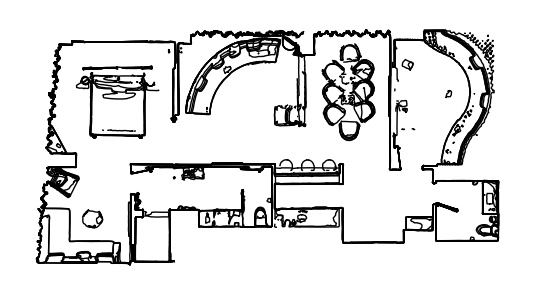
\includegraphics[width=\textwidth]{images/pose_estimator_1.png}
		\caption{}
		\label{fig:pose_estimator_1}
	\end{subfigure}
	\hfil
	\begin{subfigure}[b]{0.49\linewidth}
		\centering
		
\includegraphics[width=\textwidth]{images/pose_estimator_filled_contours.png}
		\caption{}
		\label{fig:pose_estimator_filled}
	\end{subfigure}
	\newline
	\begin{subfigure}[b]{0.49\linewidth}
		\centering
		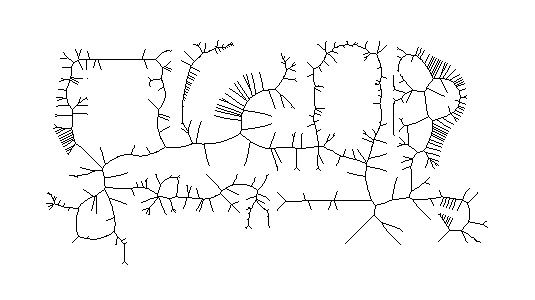
\includegraphics[width=\textwidth]{images/pose_estimator_bitmap_voronoi.png}
		\caption{}
		\label{fig:pose_estimator_voronoi_bitmap}
	\end{subfigure}
	\hfil
	\begin{subfigure}[b]{0.49\linewidth}
		\centering
		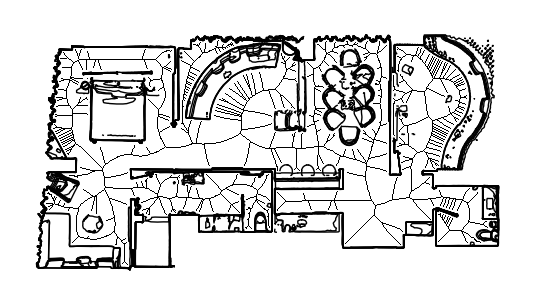
\includegraphics[width=\textwidth]{images/pose_estimator_bitmap_map.png}
		\caption{}
		\label{fig:pose_estimator_voronoi_bitmap_map}
	\end{subfigure}
	\caption{The computation of the Voronoi bitmap. In a 2D occupancy grid map of a floor (a), the free space is isolated in white (b), and the Voronoi graph is generated through Delaunay triangulation (c, d).}
	\label{fig:pose_estimator}
\end{figure}

\paragraph{Voronoi Graph Pruning and Digitization} The last step aims to extracts the graph described by the Voronoi bitmap and prune it to remove the spurious sidelines. More formally, we represent this graph as $G = (V, E)$, where the vertices are the black pixels in the Voronoi bitmap and the edges (that define symmetric relations between vertices) are implicitly stored inside nodes (each nodes specify its neighbors). 

To build a graph starting from a Voronoi bitmap (Fig. \ref{pose_estimator_bitmap}), we parse the image to build an instance node for each black pixel in the bitmap, adding them to a graph object. The \textsf{node} and \textsf{graph} classes are implemented in a file called \textsf{utilities/graph.py} of \textit{gibson-env-utilities} package. Each node is described by its coordinates in the image expressed in pixel. Then, the method proceeds with the identification of adjacent nodes that compose the graph. For each node, the approach searches the neighboring nodes inside the $3 \times 3$ pixels area centered in the current node's image coordinates. If a pixel in such area belongs to the Voronoi bitmap, the correspondent node is added to the neighbors' list of the current node and vice-versa, creating a double connection between them. The graph can be composed of multiple sub-components disconnected from each other. In other words, the initial graph $G = (N, V)$ is partitioned in multiple sub-graphs $g_1, g_2, ..., g_n$, where each sub-graphs $g_i$ is a connected component formed by a sub-set of nodes $g_i \in N \setminus \bigcup_{y=1}^{n} g_{y}, \mid y  \neq i$. Initially, the method preserves all the sub-graphs. 

The algorithm proceeds pruning the spurious sidelines. To do this, the method parses each sub-graph to recursively remove each node with a single neighbor. In other words, when the recursive function encounters the end of a sideline, it deletes the last node and consequently removes the others until the line beginning, where there is a crossroads. A plot of the pruned graphs is shown in Fig. \ref{fig:pose_estimator_pruned_lines}. 

Then the graph is printed in a new Voronoi bitmap to be further refined. The new image is subject to a dilation operation immediately followed by an image skeletonization. These two operations are necessary to obtain a bitmap Voronoi graph as clean and uniform as possible. The images dilation is performed through the OpenCV's \textsf{dilate} method, applied with a $3 \times 3$ kernel, while the skeletonization is implemented by a function provided by scikit-image\footnote{The scikit-image website: \url{https://scikit-image.org/}.}, a library designed for image processing.
Since the skeletonization function requires a binary image expressed in $[0, 1]$ range, the Voronoi bitmap is converted in a binary image encoded in such interval. After this operation, the image is re-converted in the OpenCV's format, in which pixels can assume a value between 0 and 255. The skeletonized Voronoi bitmap is shown in Fig. \ref{fig:pose_estimator_skelethon}. 

Finally, the last pruned and skeletonized Voronoi bitmap is re-parsed to build a new and more refined Voronoi graph, using the same procedure previously explained. A representation of the final graph can be seen in Fig. \ref{fig:pose_estimator_skelethon_map}. 
 
\begin{figure}[h!]
	\centering
	\begin{subfigure}[b]{0.49\linewidth}
		\centering
		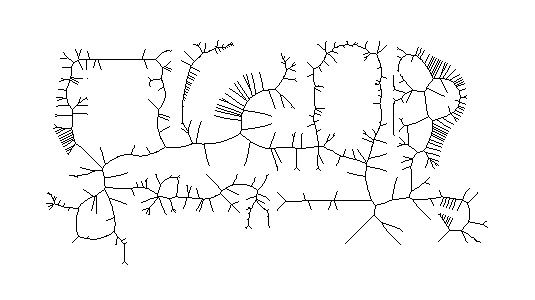
\includegraphics[width=\textwidth]{images/pose_estimator_bitmap_voronoi.png}
		\caption{}
		\label{fig:pose_estimator_bitmap}
	\end{subfigure}
	\hfil
	\begin{subfigure}[b]{0.49\linewidth}
		\centering
		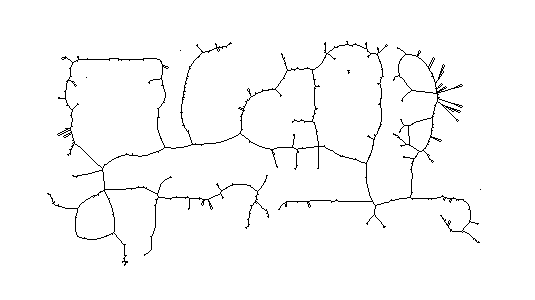
\includegraphics[width=\textwidth]{images/pose_estimator_pruned_lines.png}
		\caption{}
		\label{fig:pose_estimator_pruned_lines}
	\end{subfigure}
	\newline
	\begin{subfigure}[b]{0.49\linewidth}
		\centering
		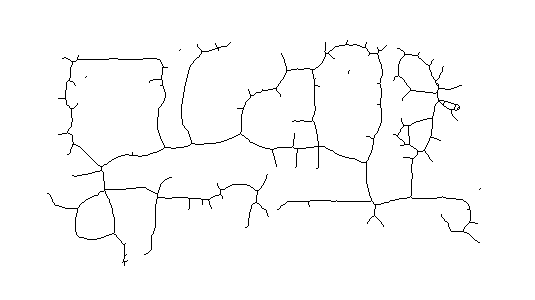
\includegraphics[width=\textwidth]{images/pose_estimator_skelethonization.png}
		\caption{}
		\label{fig:pose_estimator_skelethon}
	\end{subfigure}
	\hfil
	\begin{subfigure}[b]{0.49\linewidth}
		\centering
		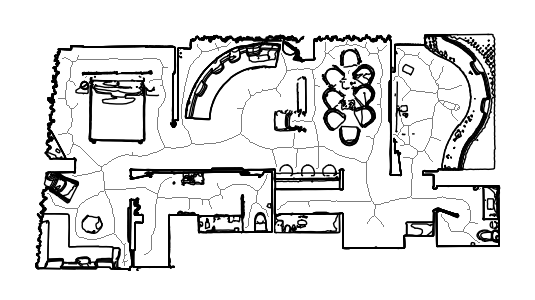
\includegraphics[width=\textwidth]{images/pose_estimator_skelethon_map.png}
		\caption{}
		\label{fig:pose_estimator_skelethon_map}
	\end{subfigure}
	\caption{The steps for pruning the Voronoi bitmap. The initial image (a) is digitized and pruned using a recursive function to remove the side lines (b). Then, the Voronoi graph is printed in a new image and skeletonized using scikit-image function (c, d). }
\end{figure}

\newpage

\paragraph{Voronoi Graph Sub-sampling} The last step performed by Pose Estimator concerns sub-sampling the Voronoi graph to extract the positions from which collect the visual dataset. As mentioned in the previous paragraph, the Voronoi graph is composed of multiple sub-graphs, that are not connected with each other. 

At first, the method discards all the sub-graphs except the longest one. Then, the approach extracts from the Voronoi graph a list of positions divided by a certain distance. The distance value is passed as a hyper-parameter, called \textsf{interval}, that controls the number and the granularity of the extracted location. The Voronoi graph is composed of multiple nodes that define points in the simulated environment. This procedure starts from an initial node described with its coordinates in the Voronoi bitmap and calculates its position in the simulated environment using the map's metadata (the map's origin and the scale). After that, the method begins to walk through the graph until a certain distance has been reached: at this point a position is sub-sampled. The method runs until the entire graph has been traversed, returning a list of positions equally spaced in the Voronoi graph (as shown by Fig. \ref{fig:pose_estimator_subsampled}). The distance between two adjacent nodes is computed by calculating the length of the legs of the right triangle between two bridges and applying the Pythagorean theorem to find the hypotenuse. Typically, the selected positions are located along the edge that connects two adjacent vertices. The conversions between the Voronoi bitmap coordinates (expressed in pixels) and the simulated coordinates (in meters) are performed by the \textsf{Coordinates} class, coded inside the \textsf{utilities/graph.py} file of \textit{gibson-env-utilities} package.

\begin{figure}[h!]
	\centering
	\begin{subfigure}[b]{0.49\linewidth}
		\centering
		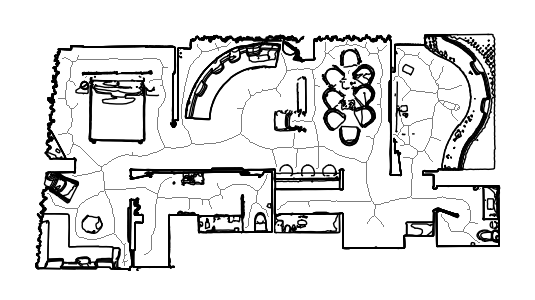
\includegraphics[width=\textwidth]{images/pose_estimator_skelethon_map.png}
		\caption{}
		\label{fig:pose_estimator_voronoi_graph}
	\end{subfigure}
	\hfil
	\begin{subfigure}[b]{0.49\linewidth}
		\centering
		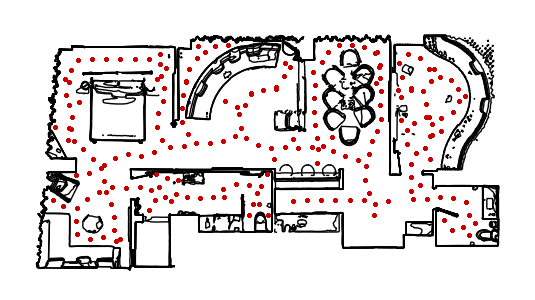
\includegraphics[width=\textwidth]{images/pose_estimator_subsampled.png}
		\caption{}
		\label{fig:pose_estimator_subsampled}
	\end{subfigure}
	\caption{The sub-sampling of the Voronoi graph.}
\end{figure}

\section{Dataset}

This thesis proposes a module to detect doors in autonomous mobile robots. Our detector, as described in Sec. \ref{sec:doors_detector}, is based on DETR, a deep end-to-end module based on Transformers \cite{transformer} that performs object detection in RGB images. In a deep learning application, the dataset plays a crucial role to determine the final results. 

The virtualization environment used in this thesis (the modified version of Gibson described in Sec. \ref{sec:new_gibson_version}) offers three types of data during a simulation run: RGB images, depth data, and semantic information. The RGB images are tri-dimensional vectors $W \times H \times 3$, where $W = H$ and the last dimension contains the pixels' colors (red, green and, blue). Depth data are encoded in bi-dimensional array with the same dimensions as the RGB images. In this way, a depth value is assigned to each pixel. Finally, semantic information is furnished in other RGB images, where the pixels are colored according to the object categories they belong to. Gibson provides 40 object categories (including doors), tagged with a numeric code. In the semantic images, the numerical code of each category is converted in an RGB color with the following procedure:

\begin{equation}
\label{eq:pareto mle2}
\begin{aligned}
B &= (\text{ID}) &\mod 256, \\
G &= (\text{ID} \gg 8) &\mod 256, \\
R &= (\text{ID} \gg 16) &\mod 256,
\end{aligned}
\end{equation}
where ID is the object category code and $\gg$ represents the bitwise right shift operation. 

In this section, we present the framework we develop to manage the vision dataset collected in this thesis. Then, we proceed by describing the dataset labeling procedure, reporting the difficulties encountered during this phase, and defining the final dataset's composition.

\subsection{The Dataset Management Framework}
\label{sec:generic_dataset}
In the initial phase of this thesis, we did not know how the final visual dataset was composed and what data characterized the collected examples. To overcome this uncertainty, we develop \textit{generic-dataset}\footnote{The generic-dataset repo: \url{https://github.com/micheleantonazzi/generic-dataset}.}, a configurable framework that automatically generates the code and the necessary classes to manage a dataset of any kind. This is possible using the \textit{meta-programming} paradigm offered by Python. Meta-programming is a technique in which computer programs have the ability to generate new code, create other programs, and modify their internal structure while running. This allows programs greater flexibility to efficiently handle new situations without recompilation. 

In Python, the meta-programming paradigm is implemented using \textit{decorators} and \textit{meta-classes}. A decorator allows programmers to modify the behavior of functions or classes. In other words, a decorator wraps an entity into a function in order to extend the behavior of the wrapped function or class, without permanently modifying it. The meta-classes, otherwise, represent a further implementation of meta-programming. In Python, everything is an object and classes are objects as well. A class in Python must have a type and it is an instance of another super-type, called meta-class. In simple terms, a meta-class is the definition of a class. The default meta-class which is responsible for making classes is called \textit{type}. Fig. \ref{fig:metaclass} visually explains the concept just reported: an object is an instance of a class and a class is an instance of a meta-class.

\begin{figure}[h!]
	\centering
	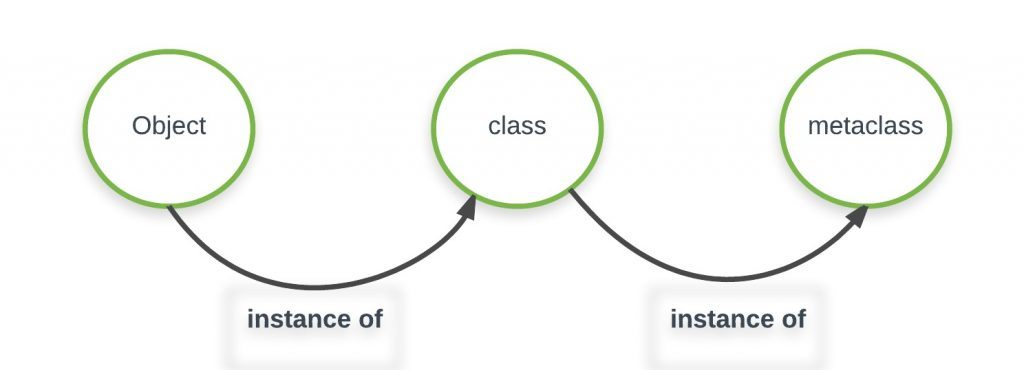
\includegraphics[width=\textwidth]{images/metaclass-hierarchy.jpeg}
	\caption{The hierarchy of objects, classes and meta-classes.}
	\label{fig:metaclass}
\end{figure}

Thanks to meta-programming, the programmer can write its custom meta-classes to modify the way from which classes are generated by performing extra actions or injecting code. By exploiting this principle, the \textit{generic-dataset} framework offers an intuitive API that creates a custom class to model a particular examples' type of a generic dataset. To do this, this API, implemented by a \textsf{SampleGenerator} object, creates a meta-class according to the directions of the programmer, that defines the final desired class to deal with precise dataset's examples. In the constructor of \textsf{SampleGenerator}, the user specifies the name of the generated sample class and the label set. In this way, both regression or classification problems can be modeled. In a regression problem, the labels are real numbers and the label space is typically infinite. In this first case, the label set passed to the constructor must be empty. Otherwise, in a classification problem, the label set must contain all the possible labels that an example can assume. The programmer can also add data fields to the final generated class, specifying their name and type. In this case, the framework automatically generates useful methods to manipulate the custom fields (like getters and setters functions). Furthermore, the user can add custom methods to the final class in order to manipulate the example's fields. Finally, using the \textsf{generate\_sample\_class} method, \textsf{SampleGenerator}, the user obtains the generated custom class (which is an instance of the configured meta-class) which models a specific type of example. The instances of the generated class, that deal directly with the examples, are thread-safe. The generated class automatically implements this feature by assigning a lock to each data field. Then, each method is decorated with a function that acquires the locks of the fields used within each method before execution and then releases them. Also, the custom methods can be synchronized by specifying the name of the used fields.

Despite we did not know the exact final composition of our dataset, surely we will deal with image manipulation. To address this requirement,  \textit{generic-dataset} offers a useful utility to manipulate RGB images, that in Python are commonly stored in NumPy arrays. This utility, implemented by the \textsf{DataPipeline} class, generates an elaboration pipeline to modify a NumPy array. A pipeline consists of a series of operations performed consecutively that can be executed in CPU or in GPU according to the programmer's needs without changing the code. This is possible using CuPy\footnote{The CuPy web page: \url{https://cupy.dev/}.}, an open-source array library for GPU-accelerated computing with Python. The CuPy's interface is highly compatible with NumPy, allowing to write agnostic programs which can be executed in CPU or GPU by replacing the engine (NumPy or CuPy), without any code change. A pipeline can be customized by adding functions to modify the initial array and then executed using the \textsf{run} method. If the \textsf{use\_gpu} flag is set as \textsf{False}, the pipeline is synchronously executed in the CPU. Otherwise, if such flag is \textsf{True}, the operations are asynchronously performed by the GPU, so the user must synchronize the two elaboration units through the \textsf{get\_data} method. This mechanism is integrated into the class generated by \textsf{SampleGenerator}. It offers the possibility to automatically create an elaboration pipeline for the fields of the generated sample class. In addition, pipelines are protected with a dedicated lock which prevents data access and modification when during the execution of the correspondent pipeline.

The \textit{generic\_dataset} framework provides a mechanism to manage the dataset's persistence. It automatically organizes the folder hierarchy to store and organize the dataset and offers the necessary methods to save and load the examples. The classes generated by \textsf{SampleGenerator} are sub-type of \textsf{GeenericSample} class, which provides a utility method to manage an example instance class of any kind. When the programmer adds a new field to the generated class, it must specify if it belongs to the dataset and, if so, it must provide the necessary functions for saving and loading such data type to the disk. The dataset folder hierarchy is organized as follows. The main directory is divided into sub-folders, that could specify different data categories or different moments in which the data are collected. Then, for a classification problem, the samples are divided into another level of sub-directories according to their label. Otherwise, in a regression task, the samples are saved in the same directory and the labels are stored in a dedicated file. Finally, the examples' fields are saved in different folders and the files inside them are named to reconstruct the acquisition order. More precisely, the file name contains two counters: the relative count and the absolute count. The first indicates the example's number based in its label's folder while the latter is the absolute count of the sample over all dataset. For a regression problem, these two values are equal because all examples belong to the same directory. Fig. \ref{fig:structuredataset} visually explain the folder hierarchy of a classification (Fig. \ref{fig:structureclassification}) and a regression (Fig. \ref{fig:structureregression}) problem. The entire dataset can be managed by an instance of \textsf{DatasetManager} class, while each folder at the first nesting level is controlled by an instance of \textsf{DatasetFolderManager}.

\begin{figure}[h!]
	\centering
	\begin{subfigure}[b]{0.5\textwidth}
		\dirtree{%
			.1 MAIN\_DATASET\_FOLDER.
			.2 FOLDER\_1.
			.3 0.
			.4 FIELD\_1.
			.5 field\_name\_rc\_ac.
			.5 field\_name\_rc\_ac.
			.5 \vdots.
			.4 FIELD\_2.
			.5 \vdots.
			.3 1.
			.4 FIELD\_1.
			.5 \vdots.
			.4 FIELD\_2.
			.5 \vdots.
			.2 FOLDER\_2.
			.3 \vdots.
			.2 \vdots.
		}
		\caption{}
		\label{fig:structureclassification}
	\end{subfigure}
	\begin{subfigure}[b]{0.4\textwidth}
		\dirtree{%
			.1 MAIN\_DATASET\_FOLDER.
			.2 FOLDER\_1.
			.3 LABEL.
			.4 label\_rc\_ac.
			.4 label\_rc\_ac.
			.4 \vdots.
			.3 FIELD\_1.
			.4 field\_name\_rc\_ac.
			.4 field\_name\_rc\_ac.
			.4 \vdots.
			.3 FIELD\_2.
			.4 field\_name\_rc\_ac.
			.4 field\_name\_rc\_ac.
			.4 \vdots.
			.2 FOLDER\_2.
			.3 \vdots.
			.2 \vdots.
		}
		\caption{}
		\label{fig:structureregression}
	\end{subfigure}
	\caption{The structure of a binary classification dataset (a) and a regression dataset (b). The files' names are are lowercase, where \textsf{rc} indicates the relative count of an example inside its label's folder, and \textsf{ac} represents the example's absolute count. }
	\label{fig:structuredataset}
\end{figure}


\subsection{Dataset Labeling and Composition}
\label{sec:dataset_labeling}
The labeling procedure in our robotic object detection task consists of dividing the positive examples (that contain the object of interest) from the negative ones and identifying the bounding boxes around the objects' instances. A vision dataset is mainly composed of RGB images, but it must specify the coordinates of the bounding boxes and their object categories in each image.

In our first dataset definition, each example is composed of all the data provided by Gibson: an RGB image, the semantic data, and the relative semantic information. The bounding boxes coordinates are not stored in dedicated files, but they are automatically calculated using  the semantic data provided by Gibson. To do this, we developed a dedicated function through the OpenCV's methods. At first, a semantic image is binarized assigning a precise color to the pixels that belong to a door and suppressing the others. Then, this function founds the contours in the binary image using the OpenCV's \textsf{findContours} method. Finally, a bounding box is created (through the \textsf{boundingRect} method of OpenCV) for each detected contour that contains a door. This function is useful because automatically designs the bounding boxes using semantic data.

Despite the usefulness of this method, we were forced to discard it after a few experiments. The main problems regard the semantic annotations. At first,  the knowledge provided by the semantic data is are not enough informative to automatically label the dataset used in this thesis. This is because, semantic information does not specify the doors' status (open or closed) and does not include implicit doors, e.g. wall openings as described in Sec. \ref{sec:door_definition}. Furthermore, the Matterport3D scenes are categorized in an inaccurate and noisy way. The tagging procedure is extremely error-prone because the semantic information is provided by labeling the vertexes of the 3D environments' meshes. Specifically identifying objects in hundreds of thousands of vertices certainly leads to errors. Examining some collected examples, we argue that some doors end up on the wall (Fig. \ref{fig:wrong_box_1}) or are partially tagged. Furthermore, adjacent doors are difficult to distinguish and often are not clearly separated in the semantic image. Another wrong situation happens when the robot does not frame the upper door jamb. In this case, the two lateral sites are recognized as different doors because they do not share pixels in the semantic image (Fig. \ref{fig:wrong_box_2}). Due to these issues, automatically finding the bounding boxes through semantic annotation is unfeasible. As shown in Fig. \ref{fig:wrong_box}, the automatic labeling procedure using only the semantic data introduces noise that can degrade the doors detector's accuracy.

\begin{figure}[h!]
	\centering
	\begin{subfigure}[b]{\linewidth}
		\centering
		\begin{subfigure}[b]{0.32\linewidth}
			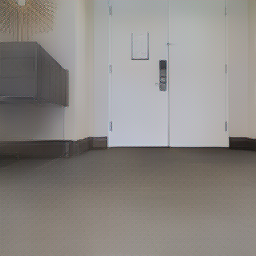
\includegraphics[width=\textwidth]{images/wrong_box_rgb_1.png}
		\end{subfigure}
		\hfil
		\begin{subfigure}[b]{0.32\linewidth}
			
\includegraphics[width=\textwidth]{images/wrong_box_semantic_1.png}
		\end{subfigure}
		\hfil
		\begin{subfigure}[b]{0.32\linewidth}
			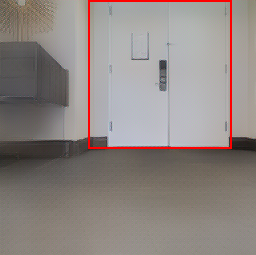
\includegraphics[width=\textwidth]{images/wrong_box_box_1.png}
		\end{subfigure}
		
		\caption{}
		\label{fig:wrong_box_1}
	\end{subfigure}
	\newline
	\begin{subfigure}[b]{\linewidth}
		\centering
		\begin{subfigure}[b]{0.32\linewidth}
			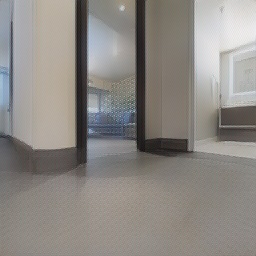
\includegraphics[width=\textwidth]{images/wrong_box_rgb_2.png}
		\end{subfigure}
		\hfil
		\begin{subfigure}[b]{0.32\linewidth}
			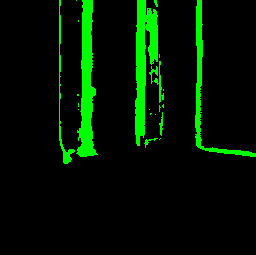
\includegraphics[width=\textwidth]{images/wrong_box_semantic_2.png}
		\end{subfigure}
		\hfil
		\begin{subfigure}[b]{0.32\linewidth}
			\includegraphics[width=\textwidth]{images/wrong_box_box_2.png}
		\end{subfigure}
		\caption{}
		\label{fig:wrong_box_2}
	\end{subfigure}

	\caption{Examples with inaccurate semantic annotations. Each row report two examples of wrong bounding boxes obtained through semantic data. From left to right, the figure shows the RGB image, the relative semantic data, and the bounding boxes derived from semantic information for each example.}
	\label{fig:wrong_box}
\end{figure}

The dataset acquisition has been performed using a hybrid method, which includes automatized procedures and the intervention of a human operator. At first, we acquired the dataset by saving all the data provided by Gibson (RGB and semantic images, and depth data). As mentioned in Sec. \ref{sec:solution}, a visual robotic dataset must contain also negative samples, so the first step concerns the discrimination between negative and positive data points. Despite the inaccuracy of the semantic data, we used them to separate the examples according to the door's presence: if the semantic image does not have pixel related to a door, the relative example is tagged as negative, as positive otherwise. Then, a human operator parses all the positive examples to define the bounding boxes and the related door's status (open or closed). For this purpose, we developed an intuitive visual tool inside the \textsf{scripts/data\_annotator.py} file of the \textit{gibson-env-utilities} package. This program loads each positive example and displays the bounding boxes extracted using the semantic data. The user can fix them by deleting the wrong bounding boxes and creating new ones, specifying also the doors' status. Some positive examples can not be used for training the doors detector module, e.g. if the robot is too close or too far to a door. In the first case, the RGB image depicts a uniform color not exposing the typical door's feature, likewise, in the second case, the doors appear as a small uniform rectangular. In particular, we discarded a door too close to the acquisition position considering the depth data: if the average distance is less that $0.30 m$, the bounding box is not displayed. Likewise, the doors too far with respect to the robot position are not considered if they cover less than $2,5\%$ of the total semantic image. In such situations, the tool we developed does not displays the bounding boxes. In this way, the user understands which doors he should not be considered. In addition, the examples with no valid doors are discarded. The final doors dataset is composed of negative and positive examples. Each example is characterized by an RBG image, the depth data, and an array with contains the bounding boxes' coordinates and the related status. In the negative examples, the list of the bounding boxes is empty.

\begin{figure}[h!]
	\centering
	\begin{subfigure}[b]{\linewidth}
		\centering
		\begin{subfigure}[b]{0.4\linewidth}
			\includegraphics[width=\textwidth]{images/correct_box_rgb_1.png}
		\end{subfigure}
		\hfil
		\begin{subfigure}[b]{0.4\linewidth}
			\includegraphics[width=\textwidth]{images/correct_box_box_1.png}
		\end{subfigure}
		\caption{}
		\label{fig:correct_box_1}
	\end{subfigure}
	\newline
	\begin{subfigure}[b]{\linewidth}
		\centering
		\begin{subfigure}[b]{0.4\linewidth}
			\includegraphics[width=\textwidth]{images/correct_box_rgb_2.png}
		\end{subfigure}
		\hfil
		\begin{subfigure}[b]{0.4\linewidth}
			\includegraphics[width=\textwidth]{images/correct_box_box_2.png}
		\end{subfigure}
	\caption{}	
	\label{fig:correct_box_2}
	\end{subfigure}

	\caption{The fixed examples of Fig. \ref{fig:wrong_box}. These two data point belong to the final dataset labeled by a human operator.}
	\label{fig:correct_box}
\end{figure}

\section{Model Evaluator}
\label{sec:model_evaluator}
This module is responsible to evaluate the performance of the door's detector trained with the collected dataset. As mentioned in Sec. \ref{sec:goals}, we collect a dataset suitable for a robotic vision application, so it is composed of positive and negative examples (where the firsts contain open or closed doors while the latter do not contain any objects of interest). The metric we implement considers these two types of examples to better evaluate the model if used by an autonomous agent. 

The evaluation method proposed by this thesis is based on the metric of Pascal VOC challenge \cite{pascal}. This metric solves several issues related to the evaluation of models that performs object detection or segmentation. In an object detection task, images contain multiple object categories or multiple instances of the same object, so a standard approach to determine which one of the $m$ classes an image contains and where it is can not be used. Furthermore, the prior distribution over different classes is significantly nonuniform so a
simple accuracy measure (percentage of correctly classified
examples) is not appropriate. During the evaluation, it is also necessary
to evaluate the trade-off between different types of classification error (e.g. false negative or false positive). The metric of the Pascal VOC challenge computes a separate ``score'' over each class to evaluate the model's performance in detecting each object category.  This metric calculates the interpolated Average Precision (AP), proposed by \citeauthor{averageprecision} in \cite{averageprecision}, over all classes in the positive images, that are closed and open door in the context of this thesis. AP is determined by the area under the precision/recall curve in the $[0, 1]$ interval. Precision and recall are two measures that differently relate the true positive (TP), false positive (FP), and false negative (FN). In an object detection task where the predictions are bounding boxes, TPs are objects correctly recognized, FNs are objects not detected, while FPs are bounding boxes that do not correspond to any object. Precision measures how accurate the predictions are, i.e. the percentage of the correct predictions over the total number of objects to detect.

It requires as input the predicted bounding boxes with their confidence score.

\begin{equation}
\label{eq:precision}
Precision = \frac{TP}{TP + FP},
\end{equation}
where $TP + FP$ represents the total number of objects to detect. Otherwise, recall measures the goodness of detections performed by the model, relating the positive classifications with the total number of model's predictions.

\begin{equation}
\label{eq:recall}
Recall = \frac{TP}{TP + FN},
\end{equation}
where $TP + FN$ is the total number of predictions performed by the model. 
To discriminate true from false positive, detections (the predicted bounding boxes) are assigned to  ground-truth objects and judged to be true/false by measuring bounding box overlap. To be considered a correct detection, the area of overlap $a_0$ between the predicted bounding
box $B_p$ and  ground-truth bounding box $B_{gt}$ must exceed a threshold, set as 0.5 in the Pascal VOC challenge. This is the intersection over union (IoU) value:

\begin{equation}
\label{eq:iou}
a_0 = \frac{area(B_p \cap B_{gt})}{area(B_p \cup B_{gt})},
\end{equation}
where $B_p \cap B_{gt}$ denotes the intersection of the predicted and
 ground-truth bounding boxes and $B_p \cup B_{gt}$ their union. The area under the precision/recall curve is computed by is defined as the mean precision at a set of eleven equally spaced recall levels $ L = \{0, 0.1,..., 1\}$:

\begin{equation}
\label{eq:11-point}
	\text{AP} = \frac{1}{11} \sum_{r \in L} p_{interp}(r).
\end{equation}
The precision at each recall level $r$ is interpolated by taking
the maximum precision measured for which the corresponding recall exceeds $r$:

\begin{equation}
p_{interp} (r) = \max_{\tilde{r} : \tilde{r} \geq r} (\tilde{r}),
\end{equation}
where $p(\tilde{r})$ is the measured precision at recall $\tilde{r}$. 

The dataset of this thesis is composed of positive and negative images, that are treated differently by the evaluation method we propose. In the following paragraphs, we explain in detail how we evaluate the model's performance with the two different macro-categories of examples we collected (positive and negative). The evaluation procedure is implemented in a dedicated class, called \textsf{MyEvaluator}, contained in the main repository of this thesis. 

\paragraph{Positive Images} The positive images are examples that contain doors to detect. As described in Sec. \ref{sec:door_definition}, we consider two possible statuses that a door can assume: open and closed. This means that the bounding boxes in the positive images belong to a set of two different object categories: $L = \{0, 1\}$. To discriminate the background bounding boxes, the doors detector we propose does not output a third label, but it assign always a label in $L$ with  low accuracy, near to zero. 

The metric we use to evaluate the model's performance in the positive image is the same evaluation method used in Pascal VOC challenge \cite{pascal}. First of all, each image in the test set is classified by the model, and an instance of \textsf{MyEvaluator} stores the  ground-truth and the predicted bounding boxes. Then, the predicted bounding boxes are divided according to the object category the model assigns to them, in order to calculate an AP (average precision) score for each label (open and closed doors). The AP value is calculated as follow:

\begin{enumerate}
	\item the  ground-truth and the predicted bounding boxes are filtered according to their confidence value: if a detection has confidence less than a threshold, called \textsf{confidence\_threshold}, it is discarded;
	\item the remaining bounding boxes are then descending ordered according to their confidence value;
	\item  following the order determined in the previous step, the module tries to match each predicted bounding box with a  ground-truth box. The matching procedure follows the next operations:
	\begin{itemize}
		\item each predicted bounding box is compared with the  ground-truth boxes of the same image, in order to find the one with the greater intersection under union (IoU) area (Eq. \ref{eq:iou});
		\item if the greater IoU area is overcome a threshold, called \textsf{iou\_threshold}, the predicted bounding box is matched with the corresponding  ground-truth box (if it has not been previously matched);
		\item the matching procedure determines the true positive (TP) and the false positive (FP) detections: each predicted bounding box matched with a  ground-truth box is considered a TP, while a detected bounding box with no match represents a FP;
	\end{itemize}
	\item when the matching procedure ends, the  ground-truth boxes not matched  are considered as false negative (FN);
	\item the true and false positives found during the matching operations are saved in order to compute the values of precision (Eq. \ref{eq:precision}) and recall (Eq. \ref{eq:recall}) at each matching step; 
	\item the final AP score is the area under the precision/recall curve, calculated by interpolate such curve at every point (refining the 11-point interpolation performed in Pascal VOC metric expressed in Eq. \ref{eq:11-point}).
\end{enumerate} 

\begin{figure}[h!]
	\centering
	\includegraphics[width=0.8\textwidth]{images/interpolated.png}
	\caption{The interpolated precision/recall curve. The blue curve is the original curve while the red one is the interpolation. AP is the area under the interpolated curve.}
	\label{fig:interpolation}
\end{figure}

\paragraph{Negative Images} The negative images do not contains objects of interest, so they are evaluated in a different way. The procedure is inspired by the metric of Pascal VOC challenge \cite{pascal} with some refinements. As mentioned in Sec. \ref{sec:detr}, DETR outputs a fixed number of predictions for every image. The back bounding boxes do not have a dedicated label, but they are characterized by a low accuracy. First of all, the predicted bounding boxes in the negative images must represent : back. The method we propose calculate a unique AP score for all  evaluation procedure of negative 




             % Concept Preview
\chapter{Experimental Results}
\label{capitolo5}
\thispagestyle{empty}

\section{Dataset Acquisition}
\label{sec:dataset_acquisition}
The visual dataset has been collected in simulated environments from Matterport3D dataset \cite{matterport} through the modified version of Gibson (described in Sec. \ref{sec:new_gibson_version}). The entire dataset is publicly available\footnote{The dataset is downloadable \href{https://drive.google.com/file/d/1BqjBpobjKTomFjDkzhWjmCryAXOEluO2/view?usp=sharing}{here}.}The positions from which the examples are acquired are extracted from the Pose Selector, described in Sec \ref{sec:pose_estimator}. We select a set $E$ of $10$ worlds of Matterport3D dataset, where $E = \{\text{house1}, \text{house2}, \text{house7}, \text{house9}, \text{house10}, \text{house13}, \text{house15}, \text{house20}, \\ \text{house21},  \text{house22}\}$. The dataset's acquisition procedure, previously described in Sec. \ref{sec:dataset_labeling}, is now formalized by reporting the various steps and specifying the hyper-parameters' values. The collection algorithm works as follows:

\begin{enumerate}
	\item we start a simulation run with Gibson for each environment $e \in E$, where the virtualized agent is a Turtlebot2 \cite{turtlebot2};
	\item for each environment we select a set of positions through the Pose Estimator module, by setting \textsf{interval} $= 1.00m$. This means that the selected positions are spaced $1.00m$ from each other in the Voronoi graph created by Pose Estimator;
	\item during the simulation run, the robot is positioned in each location and we collect a pool of examples changing the robot orientation and the height with respect to the floor. We select a set of height values $H = \{0.10m, 0.70m\}$ and a set of 8 rotation angles $O = \{0^{\circ}, 45^{\circ}, 90^{\circ}, 135^{\circ}, 180^{\circ}, 225^{\circ}, 270^{\circ}, 315^{\circ}\}$;
	\item for each position, we collect an example for every pair height-orientation in the Cartesian product $H \times O = \{(h, o) \mid h \in H, o \in O\}$. Since $|H \times O| = 16$, we collect 16 examples for each location extracted in the previous step;
	\item as mentioned in Sec \ref{sec:dataset_labeling}, an examples is initially composed by the data provided by Gibson: an RGB image, depth data, and a semantic information contained in another RGB image;
	\item a human operator parses all the positive examples whit a dedicated tool in order to fix the bounding boxes found with the semantic annotated images, to specify the label (which means close or open doors) for each bounding box, and to highlight the implicit doors which are not tagged. During this manual labeling procedure, the user also discards the bounding boxes around not valid objects of interest, that are doors too close or too far in the RGB image. In particular, we discarded a door too close to the acquisition position considering the depth data: if the average distance is less that $0.30 m$, the bounding box is not displayed. Likewise, the doors too far with respect to the robot position are not considered if they cover less than $2,5\%$ of the total semantic image. In such situations, the tool we developed does not displays the bounding boxes. If an image has no valid doors, the entire example is discarded. Another important goal of the manual labeling procedure is to remove the corrupted or malformed images produced by Gibson;
	\item with the same tool, a human operator checks also the negative images to discard the examples with wrong RGB images; 
	\item the labeling tool automatically saves the checked examples in a new dataset folder. Finally, each example is composed by an RGB image, the depth data, and an array that contains the bounding boxes coordinates and their labels (that indicate the door's status). 
\end{enumerate}

The dataset is managed using the \textit{generic-dataset} packaged described in Sec. \ref{sec:generic_dataset}. This framework organizes the dataset persistence directory-tree by Fig. \ref{fig:organization_dataset}.

\begin{figure}[h!]
	\centering
	\begin{minipage}{7cm}
		\dirtree{%
			.1 MAIN\_DATASET\_FOLDER.
			.2 house1.
			.3 1.
			.4 rgb\_image.
			.5 rgb\_image\_rc\_ac.png.
			.5 rgb\_image\_rc\_ac.png.
			.5 \vdots.
			.4 depth\_data.
			.5 \vdots.
			.4 bounding\_boxes.
			.5 \vdots.
			.3 0.
			.4 \vdots.
			.3 \vdots.
			.2 house2.
			.3 \vdots.
			.2 \vdots.
		}
	\end{minipage}
	\caption{The structure of the visual dataset collected in this thesis. }
	\label{fig:organization_dataset}
\end{figure} 

Table \ref{tab:dataset_examples_number} reports the number of examples acquired for each environment $e \in E$, that compose the dataset we collected.

\begin{table}[h!]
	\centering
	\begin{tabular}{cccc}

	\toprule
	\textbf{Env. name} & \textbf{Positive examples} & \textbf{Negative examples} & \textbf{Total
		examples}\tabularnewline
	\midrule
	house1 & 350 & 363 & 713\tabularnewline
	house2 & 482 & 529 & 1011\tabularnewline
	house7 & 358 & 227 & 585\tabularnewline
	house9 & 774 & 410 & 1184\tabularnewline
	house10 & 446 & 308 & 754\tabularnewline
	house13 & 413 & 230 & 643\tabularnewline
	house15 & 652 & 423 & 1075\tabularnewline
	house20 & 408 & 350 & 758\tabularnewline
	house21 & 826 & 551 & 1377\tabularnewline
	house22 & 748 & 515 & 1263\tabularnewline
	\bottomrule
	\end{tabular}
	\caption{The number of examples for every environment $e \in E$.}
	\label{tab:dataset_examples_number}
\end{table}

\section{DETR Configuration}

As mentioned in Sec. \ref{sec:doors_detector}, the doors detector module proposed in this thesis is built using DETR \cite{detr}. As a reminder, DETR's architecture (described in Sec. \ref{sec:sec:detrarchitecture}) is composed by a CNN backbone (ResNet \cite{resnet}) which  provides a low dimensional representation of it. Then, the features extracted are fed into a Transformer \cite{transformer} to capture the relationships between them by reasoning over the entire image as context. Finally, the bounding boxes coordinates are inferred by a 4-layer perceptron while their labels are extracted through a linear classifier. In the following paragraphs, we describe in detail the configuration of DETR we use to run our experiments. We starts discussing the architecture of DETR. Then, we proceed describing the parameters' initialization and, finally, we report the hyper-parameter used for the training of DETR

\paragraph{DETR Architecture}
\citeauthor{detr} \cite{detr} propose 4 versions of DETR. The first one is composed by a ResNet-50 while the second has a ResNet-101 as feature extractors. The authors called these models DETR and DETR-R101 respectively. Then, the authors propose other two architectures starting from both DETR and DETR-R101. Following the work proposed in \cite{fullyconvolutional}, the authors of DETR increase the feature resolution by
adding a dilation to the last stage of the backbone and removing a stride from
the first convolution of this stage. The corresponding models are called respectively DETR-DC5 and DETR-DC5-R101. This modification
increases the resolution by a factor of two, thus improving performance for small
objects, at the cost of a 16x higher cost in the self-attentions of the encoder,
leading to an overall 2x increase in computational cost. This modification
increases the resolution by a factor of two, thus improving performance for small
objects, at the cost of a 16x factor in the self-attentions of the encoder,
leading to an overall 2x increase in computational cost. A full comparison of
FLOPs (number of floating point operations per second), FPS (frame per second), and parameters' number of these models is given in Table \ref{tab:detr_models_flops}. The authors calculate the FLOPS for first 100 images in the COCO 2017 validation set using tool \textsf{flop\_count\_operators} from Detectron2 \cite{detectron2}. We use the standard version of DETR to build the doors detector: the model's efficiency is crucial in a robotic context and the modified versions of DETR increase a lot the inference time and the memory consumed. 

\begin{table}[h!]
	\centering
	\begin{tabular}{cccc}
		
		\toprule
		\textbf{Model name} & \textbf{GFLOPS} & \textbf{FPS} & \textbf{Paramaters} \tabularnewline
		\midrule
		DETR & 86 & 28 & 41M\tabularnewline
		DETR-DC5 & 187 & 12 & 41M\tabularnewline
		DETR-R101 & 152 & 20 & 60M\tabularnewline
		DETR-DC5-R101 & 233 & 10 & 60M\tabularnewline
		\bottomrule
	\end{tabular}
	\caption{The comparison between the four architecture of DETR. Table from \cite{detr}.}
	\label{tab:detr_models_flops}
\end{table}

\paragraph{DETR's Configuration}
\label{sec:detr_configuration}
We do not retrain the entire model but we load the pre-trained version of DETR furnished by the authors. This is because training DETR from scratch is unfeasible. First of all, as reported in \cite{surveytransformer}, the Transformers used in Computer Vision need wide training datasets. As a prove, DETR is trained for 300 epochs using the COCO 2017 dataset \cite{coco} which contains for about 118K of training images. This procedure takes 3 days on a cluster with 16 Tesla V100 GPUs and a batch size of 64 (4 images for each GPU). Since we have a small doors dataset (with for about 8K examples) and a limited computing power, we fine-tune DETR with a few data to resolve a more refined task (detecting doors). Fine-tuning a model pre-trained with a dataset like Imagenet \cite{imagenet} has become a common technique for solving computer vision tasks \cite{verydeepimagenet, resnet, fasterrcnn, yolo, yolov2}. We adopt the same strategy, with the difference that DETR is pre-trained using COCO dataset.

\paragraph{DETR Hyper-Parameters}
Now, we describe in detail the setting of the hyper-parameters used for training the model. We train DETR using the AdamW  \cite{adamw} optimizer implemented in PyTorch. We set AdamW with a \textsf{weight\_decay} of $1^{-4}$. The backbone and the transformers are treated slightly differently.  We train the CNN backbone with a learning rate of $10^{-6}$, while the learning rate of the Transformer is set at $10^{-5}$. The authors observe that having the backbone learning rate roughly an order of magnitude smaller than the rest of the network is important to stabilize training, especially in the first few epochs. 

As reported in Sec. \ref{sec:detrlosses}, the loss function for bounding box regression is a linear combination of $\ell_1$ and generalized IoU \cite{generalizediou} losses (Eq. \ref{eq:bounding_box_loss}). We set $\lambda_{iou} = 2$ and $\lambda_{L1} = 5$.

Another important hyper-parameter is the number of object queries. As specified in Sec. \ref{sec:detrarchitecture}, the module produce a detection for each object queries. In the original article of DETR \cite{detr}, the total number of object queries is  $N = 100$. This because, as specified by the authors, $N$ must be greater than the maximum number of objects instances in an image (the images of COCO contain up to 70 distinct objects). In our dataset, the maximum number of doors in an image is 3, so we set $N = 10$.

\paragraph{Data Augmentation} DETR \cite{detr} is a wide model that requires a huge amount of training data to converge. To overcome this issue, the authors perform an intense data augmentation of the COCO's images used for DETR's training. Another purpose of the data augmentation technique is to generalize well the problem by producing new images starting from the original ones. In this way, the model learns from different images increasing in accuracy and preventing overfitting. 

The data augmentation applied to each training image is composed by the following operations:

\begin{enumerate}
	\item \textbf{horizontal flip:} at first, the authors apply a horizontal flip to the image with a probability of $0.5$;
	\item \textbf{random select:} now, the data augmentation proceeds choosing one of the following algorithms with a probability of $0.5$:
	\begin{enumerate}
		\item \textbf{random resize:} the image is randomly resized such that the shortest side is at least 480 and at most 800 pixels while the longest at most 1333;
		\item \textbf{random size crop:} the image, which is initially resized with the same procedure of the previous operation, is cropped to a random rectangular patch (with random sizes) which is then resized again;
	\end{enumerate} 
	\item finally, the image is normalized. Normalizing the images means transforming the images into such values that the mean and standard deviation of the image become 0.0 and 1.0 respectively. First of all, an image $W \times H \times 3$ is converted to a tensor with shape $3 \times H \times W $ and the integer pixels are scaled in the $[0.0, 1.0]$ interval. Then, each input channel is subtracted by the channel mean and then the result is divided by the channel standard deviation. The channels' mean and standard deviation used by the authors are calculated over the Imagenet dataset \cite{imagenet}.
\end{enumerate}

During the firsts experiments, we argue that this massively data augmentation is not appropriate in the context of this thesis. First of all, we use the pre-trained DETR version on COCO 2017 dataset, so the model already has a good initialization of the weights. Furthermore, we use a dataset less than one order of magnitude with respect to COCO. This means that we do not have enough examples for making a data modification like those performed in the original train of DETR. Another important issue regards the crop procedure with respect to the our objects of interest. In the context of this thesis, we aim to detect open or closed doors, that are typically big objects in images. By random cropping a frame, the door's features may be insufficient for a successful model's training. For these reasons, we perform a reduced data augmentation. With a probability of $0.5$, we modify the image with a random horizontal flip followed by a random resize operation; otherwise, the image is not modified. Finally, we normalize the frame with mean and standard deviation of Imagenet dataset. Since our images are smaller ($256 \times 256 \times 3$) than those of COCO, the random resize is performed in a different range, between 256 and 576 pixels. 

\section{DETR Analysis}

Before proceeding with the evaluation of DETR over the collected dataset, we test the proposed doors detector with a well known doors dataset, called \textit{DeepDoors2} \cite{deepdoors2}, which is freely available on Github\footnote{The DeepDoors2 Github page: \url{https://github.com/gasparramoa/DeepDoors2}.}. We perform this experiment to understand if DETR is trainable with a smaller dataset than COCO and to verify if it obtains good results in a doors detection task. In the following sub-sections, we describe in detail the DeepDoors2 dataset proposed in \cite{deepdoors2} and how we modify it to better approach the requirements of the task addressed by this thesis. Then, we report the results obtained by the doors detector we proposed if trained with the improved version of DeepDoors2. Finally, we further analyze the DETR's performance by visualizing the detections produced by the trained model using t-SNE \cite{tsne}.

\section{DeepDoors2 Dataset}
DeepDoors2 is a visual dataset which contains 3000 labeled examples composed by  RGB images (with dimension of $480 \times 640 \times 3$), depth data, and the relative semantic information encoded in another RGB images. The labels provided by the authors indicates also the doors' status, which can be open, semi-open, and closed (Fig. \ref{fig: open_semi_closed}). The examples are equally divided over these doors' categories.  This dataset is constituted by 3 parts, a 2D and 3D image classification part, a semantic segmentation part and an object detection part. For the first two parts, the authors use their previous
dataset, published in \cite{deepdoors1}, and improve it by collecting more data and annotating more images. The third part was built by labeling the image of the classification part. This dataset was captured in different indoor environments (universities, public spaces, and houses) using a portable system constituted by a Raspberry Pi 3 B+ with a 3D Realsense Camera, model D435. The authors captured several images of doors and their surroundings with different textures and sizes, sometimes obstructed by obstacles (e.g. chairs, tables, furniture, and even persons). The authors also changed the pose to get different perspectives on the same door. 

\begin{figure}[h!]
	\begin{subfigure}[b]{0.32\linewidth}
		\includegraphics[width=\linewidth]{images/deep_doors_2_open.png}
		\caption{}
	\end{subfigure}
	\hfil
	\begin{subfigure}[b]{0.32\linewidth}
		\includegraphics[width=\linewidth]{images/deep_doors_2_semiopen.png}
		\caption{}
	\end{subfigure}
	\hfil
	\begin{subfigure}[b]{0.32\linewidth}
		\includegraphics[width=\linewidth]{images/deep_doors_2_closed.png}
		\caption{}
	\end{subfigure}
	\caption{Labeled images from DeepDoors2 dataset. (a) An open door, (b) a semi-open door, and (c) a closed door. Green, blue, and red bounding boxes represent open, semi-open, and closed doors respectively.}
	\label{fig: open_semi_closed}
\end{figure}

The object detection part of DeepDoors2 dataset is annotated with an automatic procedure that finds bounding boxes around doors using the semantic data. The labeling algorithm implemented by the authors finds a single door for each image, but we argue that a single example can depict multiple doors instances with different statues (Fig. \ref{fig:relabeling_deepdoors2}). Due to this fact, we manually re-label the entire dataset with the visual tool described in Sec. \ref{sec:dataset_labeling}. Furthermore, we re-organize the dataset according to the standard defined by the \textit{generic-dataset} framework reported in Sec. \ref{sec:generic_dataset}. We release the re-labeled version of DeepDoors2 dataset\footnote{The DeepDoors2 re-labeled dataset can be downloaded \href{https://drive.google.com/file/d/1wSmFUHF9aSJkomwFdOmepMevBvkRpf3D/view?usp=sharing}{here}.} and the necessary Python code\footnote{The DeepDoors2 re-labeled source code: \url{https://github.com/micheleantonazzi/deep-doors-2-labelled}.} to manage it. The final DeepDoors2 dataset is composed oh 2998 examples, while each of them include an RGB image with dimension $480 \times 640 \times 3$, a matrix $480 \times 640$ which contains the depth data, and a list with the bounding boxes' coordinates and the relative labels (open, semi-open, or closed door). 

\begin{figure}[h!]
	\centering
	\begin{subfigure}[b]{\linewidth}
		\hfil
		\begin{subfigure}[b]{0.26\linewidth}
			\includegraphics[width=\linewidth]{images/deep_doors_2_labeling1.png}
		\end{subfigure}
		\hfil
		\begin{subfigure}[b]{0.26\linewidth}
			\includegraphics[width=\linewidth]{images/deep_doors_2_labeling1_semantic.png}
		\end{subfigure}
		\hfil
		\begin{subfigure}[b]{0.26\linewidth}
			\includegraphics[width=\linewidth]{images/deep_doors_2_labeling1_correct.png}
		\end{subfigure}
		\hfil
		\caption{}
	\end{subfigure}
	\newline
	\begin{subfigure}[b]{\linewidth}
		\hfil
		\begin{subfigure}[b]{0.26\linewidth}
			\includegraphics[width=\linewidth]{images/deep_doors_2_labeling2.png}
		\end{subfigure}
		\hfil
		\begin{subfigure}[b]{0.26\linewidth}
			\includegraphics[width=\linewidth]{images/deep_doors_2_labeling2_semantic.png}
		\end{subfigure}
		\hfil
		\begin{subfigure}[b]{0.26\linewidth}
			\includegraphics[width=\linewidth]{images/deep_doors_2_labeling2_correct.png}
		\end{subfigure}
	\hfil
		\caption{}
	\end{subfigure}
	\caption{Two examples of wrong labeled images from the original version of DeepDoors2 dataset. The left figures in each row represents the bounding boxes found with the depth data encoded in the middle images. The figures on the right depict the fixed labeled images of our version DeepDoors2.}
	\label{fig:relabeling_deepdoors2}
\end{figure}

\subsection{DETR's Performance on DeepDoors2}

Before proceeding with other experiments, we test DETR on the relabeled version of DeepDoors2 to verify if it converges with such a small dataset and if it has acceptable performance in a doors detection task. We randomly split the dataset into a training set of the $80\%$ of examples and a test set with the remaining ones. We train DETR for 40 epochs with a batch size of 1. We report the DETR loss function (Eq. \ref{eq:detr_loss}) during training both for train and test sets in Fig. \ref{fig:deep_doors2_loss}.

\begin{figure}[h!]
	\centering
	\includegraphics[width=\linewidth]{images/deep_doors_2_loss.png}
	\caption{The loss function during the training of DETR.}
	\label{fig:deep_doors2_loss}
\end{figure}

We evaluate the trained version of DETR with the Pascal VOC metric \cite{pascal} as described in Sec. \ref{sec:model_evaluator}. We set the \textsf{iou\_threshold}$ = 0.9$ and the \textsf{confidence\_threshold} $= 0.5$. Table \ref{tab:deep_doors2_results} reports the AP score for each object category (open, semi-open, and closed doors) and the data to calculate it, such as the total number of the ground-truth bounding boxes, the true positive, and the false positive detections performed by the model. The plot of the interpolated precision/recall curves for each category is shown in Fig. \ref{fig:deep_doors2_ap_plot}.

\begin{table}[h!]
	\centering
	\begin{tabular}{cccccc}
		
		\toprule
		\textbf{Label} & \textbf{AP} & \textbf{N. Positives} & \textbf{TP} & \textbf{FP} & \textbf{FN}\tabularnewline
		\midrule
		Closed door (0) & 90 & 234 & 214 & 45 & 20 \tabularnewline
		Semi-open door (1) & 83 & 198 & 169 & 33 & 29 \tabularnewline
		Open door (2) & 85 & 243 & 214 & 66 & 29 \tabularnewline
		\bottomrule
	\end{tabular}
	\caption{The performance of DETR trained on the DeepDoors2 dataset.}
	\label{tab:deep_doors2_results}
\end{table}

\begin{figure}[h!]
	\centering
	\includegraphics[width=\linewidth]{images/deep_doors_2_precision_recall.png}
	\caption{The interpolated precision/recall curves about open, semi-open, and closes doors, colored in green, blue, and red respectively.}
	\label{fig:deep_doors2_ap_plot}
\end{figure} 

As shown by Fig. \ref{fig:deep_doors2_loss}, the model converges correctly and does not overfit or underfit. Both the training and test error (reported in blue and orange respectively) are low and closed to each other. As reported in Table \ref{tab:deep_doors2_results}, the proposed doors detector reaches a good accuracy for all the three door categories (open, semi-open, and closed). An AP greater that 80 is considered a good in the Computer Vision community.

\subsection{The DETR's Detection Visualization}
As mentioned in Sec. \ref{sec:detrarchitecture}, each object queries produces a detection composed by the bounding box coordinates and the relative label. To further analyze the DETR's performance, we plot in 2D the object queries classified by the Transformers using t-SNE \cite{tsne}. t-SNE (t-distributed Stochastic Neighbor Embedding) is a unsupervised and randomized technique to visualize high-dimensional data by giving each data point a location in a two or three dimensional map. It models each high-dimensional object by a two or three-dimensional point in such a way that similar objects are modeled by nearby points and dissimilar objects are modeled by distant points with high probability. This algorithm is a variation of Stochastic Neighbor Embedding (SNE) \cite{sne}. SNE starts by converting the high-dimensional Euclidean distance between all pairs of data points into conditional probabilities. More formally,  The similarity of data point $x_j$ to data point $x_i$ is the conditional probability $p_{j \mid i}$, where $x_i$ considers $x_j$ as a neighbor in proportion to a Gaussian centered in $x_i$. For nearby data points, $p_{j \mid i}$
is relatively high, whereas for widely separated data points, $p_{j \mid i}$ will be almost infinitesimal. Note that $p_{i \mid i} = 0$. For the low-dimensional counterpart of  $x_i$ and $x_j$ (denoted as $y_i$ and $y_j$), it possible to compute a similar conditional probability  $q_{j \mid i}$.
If the map points $y_i$ and $y_j$ correctly model the similarity between the high-dimensional datapoints $x_i$ and $x_j$, the conditional probabilities $p_{j \mid i}$ and $q_{j \mid i}$ will be equal. Motivated by this observation, SNE aims to find a low-dimensional data representation that minimizes the sum of the mismatches between $p_{j \mid i}$ and $q_{j \mid i}$ of all pairs of data points. A natural way to measure the distance between two probability distributions is the Kullback-Leibler diverge, which the sum is minimized by SNE using a gradient descent method.

Although SNE constructs reasonably good visualizations, it is limited by a cost function that is difficult to optimize because, if $x_i$ is an outlier data point, the value of the joint probabilities $p_{i j}$ (which defines the pairwise similarities in the between $x_i$ and $x_j$ high-dimensional space) is extremely small for all $j$. To overcome this problem, the authors of t-SNE defines the joint probabilities $p_{i j}$ in the high-dimensional space as the symmetrized conditional probability:

\begin{equation}
 p_{i j} = \frac{p_{j \mid i} + p_{i \mid j}}{2n}.
\end{equation}
This ensure that, if $x_i$ is an outlier data point, $\sum_{j} p_{i j} > \frac{1}{2n}$.

Another issue of SNE is the ``crowding problem''. It is difficult to correctly ``scale'' long and short distances of points in low-dimensions. The area in a low-dimensional space that is available to accommodate moderately distant
data points in high-dimensional map will not be nearly large enough compared with the area available to accommodate nearby data points. Otherwise, if we want to model the small distances accurately in the map, most of the points that are at a moderate distance from a data point $i$ will have to be placed much too far away in the two-dimensional map. To overcome this problem, the authors of t-SNE use the Student t-distribution (with a single degree of freedom) instead of the Gaussian in the conversion between Euclidean distance and probability. The Student distribution ``falls'' quickly and has a ``long tail'', so points will not be squashed into a single point. 

The t-SNE algorithm initially calculates the symmetric probabilities $p_{i j}$ between all the high-dimensional data points of a given dataset. Then, it performs multiple iterations in which calculates the low-dimensional affinities values $q_{i j}$, performs the SGD algorithm to optimize the distance between the pairs of $p_{i j}$ and $q_{i j}$.

As previously anticipated, we plot the output embeddings of the Transformer with t-SNE in a two-dimensional space. We train DETR for 40 epochs with a batch size of 1 using 80\% of the examples of the re-labeled version of DeepDoors2. Then, we classify both the training set and the test set (composed the 20\% of the remaining examples) with the trained model, saving the object queries modified by the Transformer. Finally, we clusterize only the predictions with the highest accuracy of every image using the \textit{scikit-image} implementation of t-SNE, by setting 2 different values for perplexity: 30 and 100. Before clusterizing them through t-SNE, we reduce their dimensionality to 50 using the Principal Components Analysis (PCA) \cite{pca}, which projects a data point onto only the first few principal components preserving as much of the data's variation as possible. 

\begin{figure}[h!]
	\centering
	\includegraphics[width=\linewidth]{images/deep_doors_2_tsne_trainset.png}
	\caption{The plot of the Transformer's output embeddings using t-SNE over the training set.}
	\label{fig:tsne_deep_doors2_train}
\end{figure}

\begin{figure}[h!]
	\centering
	\includegraphics[width=\linewidth]{images/deep_doors_2_tsne_testset.png}
	\caption{The plot of the Transformer's output embeddings using t-SNE over the test set.}
	\label{fig:tsne_deep_doors2_test}
\end{figure}
 
The Figures \ref{fig:tsne_deep_doors2_train} and \ref{fig:tsne_deep_doors2_test} show that DETR produce useful features encoding to separate the open, semi-open, and closed doors. Thanks to t-SNE, we argue that the objects queries classified by the Transformer are clearly separated in three distinct clusters examining both the training and the test sets (as expected looking the good results reported in Tab. \ref{tab:deep_doors2_results}). Since the AP scores are not equals to 1, there are some spurious detections in the t-SNE's plots that likely lead to false positives.

\section{One-Shot Incremental Learning}

As mentioned in Sec. \ref{sec:solution}, we not only offer a deep learning module for finding doors, but we also propose a technique for increasing the detector's performance exploiting a specific deployment scenario for a mobile robot as  explained in Sec. \ref{sec:deploymentscenario}. The idea we follow is that a machine learning model for finding doors used by an autonomous agent is initially trained on a general dataset to be suitable for any context of use. At best of our knowledge, the module's performance can be variable according to visual aspect of the scene in which the robot operates. To increase the detector's accuracy, we propose a method to specialize the generic model for the specific environment in which the robot is deployed. This technique, which we call \textbf{one-shot incremental learning}, consists on fine-tune a generic doors detector with a new dataset acquired from the new environment. This thesis also investigates the necessary amount of unseen examples to obtain a significant performance improvement.

To successfully evaluate the \textbf{one-shot incremental learning} technique, the experimental phase of this thesis emulates the requirements for ideal deployment scenario for a mobile robot using the dataset of doors we collected. As reported in Sec. \ref{sec:dataset_acquisition}, the visual doors dataset has been acquired from set $E$ of 10 different environments from Matterport3D \cite{matterport} virtualized through the modified version of Gibson \cite{gibson} (described in Sec. \ref{sec:new_gibson_version}). The examples are both positive and negative and they are divided according the environment of belonging. For each environment $e \in E$, the entire dataset $D_{e}$ is split into 2 sub-sets $G_e$ and $S_e$, where $G_e$ contains all the examples that do not belong to the selected environment $e$, while $S_e$ is composed of the images collected from $e$. Then, $G_e$ is divided into 2 sub-sets $G^{P}_e$ and $G^{N}_e$: the first contains only the positive examples while the latter only the negative ones not acquired in the environment $e$. Likewise, $S_e$ is split in $S^{P}_e$ and $S^{N}_e$ that respectively contain the positive and the negative examples of the environment $e$. Finally, 4 sub-sets are extracted from $S^{P}_e$, which are $S^{P}_{e, 1}$, $S^{P}_{e, 2}$, $S^{P}_{e, 3}$, and $S^{P}_{e, 4} $. They are composed of the 25\% of the examples of $S^{P}_e$. We use this dataset division to perform a series of two experiments for each environment:



\begin{itemize}
	\item \textbf{Experiment 1:} at first, we train for 40 epochs a general doors detector with $G^{P}_e$, that contains the positive examples that do not belong to the environment $e$. We use the configuration of DETR reported in Sec. \ref{sec:detr_configuration}. Then, we evaluate this model using the metric explained in Sec. \ref{sec:model_evaluator}, with a test set composed by $S^{P}_{e, 4}$ and $S^{N}_e$, that respectively contains the 25\% of the positive all the negative examples from the examples collected in $E$. We formally call this experiment \textsf{GD} (general doors detector). 
	
	\item \textbf{Experiment 2:} then, we perform a series of 3 fine-tune operations on the module trained in the previous experiment. We re-train (using the parameters reported in Sec. \ref{sec:detr_configuration}) for 20 epochs  the pre-trained module producing 3 fine-tuned versions of the generic doors detector using three different training sets $T$. At first, we set $ T= \big\{S^{P}_{e, 1}\big\}$, then $T=\big\{S^{P}_{e, 1} \cup S^{P}_{e, 2}\big\}$, and finally $T=\big\{S^{P}_{e, 1} \cup S^{P}_{e, 2} \cup S^{P}_{e, 3}\big\}$, so we fine-tune the general model by employing the  25\%, 50\%, and the 75\% of the positive samples collected in $e$. As the previous experiment, each of the fine-tuned doors detector is evaluated through the metric described in Sec. \ref{sec:model_evaluator} using the remaining 25\% of the positive examples and all the negative images, contained in $S^{P}_{e, 4}$ and $S^{N}_e$ respectively. We refer to these 3 fine-tune detectors as \textsf{FD\textsubscript{25}}, \textsf{FD\textsubscript{50}}, and \textsf{FD\textsubscript{75}}. 

\end{itemize}

In simple terms, we built 4 different doors detector for each environment in the collected dataset: the general doors detector (\textsf{GD}) trained without images acquired in the selected environment and other 3 detectors trained by fine-tuning the general model with the 25\% (\textsf{FD\textsubscript{25}}), 50\% (\textsf{FD\textsubscript{50}}), and 75\% (\textsf{FD\textsubscript{75}}) of the examples of the selected environment. All these model are tested with the remaining 25\% of the samples of the current environment ($S^{P}_{e,4}$) and all the negative images of the current environment ($S^{N}_{e}$).

\paragraph{House13 Analysis}

We report in detail the analysis of a single environment $e\in E$, house13. As previously mentioned,  First of all, we test the performance of the trained detectors using the metric explained in Sec. \ref{sec:model_evaluator}. Table \ref{tab:house13_results} shows the results obtained with house13, reporting the AP scores, the total number of ground-truth positive bounding boxes, the true positives detections, and the false positive detections predicted by the models. 

\begin{table}[h!]
	\centering
	\begin{tabular}{ccccccc}
		
		\toprule
		\textbf{Env.} & \textbf{Exp.} & \textbf{Label} & \textbf{AP} & \textbf{N. Positives} & \textbf{TP} & \textbf{FP} \\
		\midrule
		\multicolumn{1}{c|}{\multirow{12}{*}{House 13}} & \multicolumn{1}{c|}{\multirow{3}{*}{\textsf{GD}}} & Negative examples (-1) & 88 & 3630 & 3320 & 310  \tabularnewline 
		\multicolumn{1}{c|}{}& \multicolumn{1}{c|}{} & Closed door (0) & 41 & 27 & 14 & 21  \\
		\multicolumn{1}{c|}{}& \multicolumn{1}{c|}{}& Open door (1) & 38 & 101 & 61 & 88  \\  \cline{2-7}
		\multicolumn{1}{c|}{}& \multicolumn{1}{c|}{\multirow{3}{*}{\textsf{FD\textsubscript{25}}}} & Negative examples (-1) & 93 & 3630 & 3452 & 178  \tabularnewline [1pt]
		\multicolumn{1}{c|}{}& \multicolumn{1}{c|}{} & Closed door (0) & 59 & 27 & 16 & 3  \\ 
		\multicolumn{1}{c|}{}& \multicolumn{1}{c|}{} & Open door (1) & 56 & 101 & 72 & 62   \\ \cline{2-7}
		\multicolumn{1}{c|}{} & \multicolumn{1}{c|}{\multirow{3}{*}{\textsf{FD\textsubscript{50}}}} & Negative examples (-1) & 94 & 3630 & 3455 & 175  \tabularnewline 
		\multicolumn{1}{c|}{}& \multicolumn{1}{c|}{} & Closed door (0) & 66 & 27 & 18 & 3  \\
		\multicolumn{1}{c|}{}& \multicolumn{1}{c|}{}& Open door (1) & 57 & 101 & 68 & 55  \\  \cline{2-7}
		\multicolumn{1}{c|}{}& \multicolumn{1}{c|}{\multirow{3}{*}{\textsf{FD\textsubscript{75}}}} & Negative examples (-1) & 93 & 3630 & 3428 & 202  \tabularnewline [1pt]
		\multicolumn{1}{c|}{}& \multicolumn{1}{c|}{} & Closed door (0) & 65 & 27 & 18 & 6  \\ 
		\multicolumn{1}{c|}{}& \multicolumn{1}{c|}{} & Open door (1) & 63 & 101 & 74 & 54   \\ 
		\bottomrule
	\end{tabular}
	\caption{The evaluation of the \textbf{one-shot incremental learning} on house13.}
	\label{tab:house13_results}
\end{table}

The, we report the plots of the loss function (Eq. \ref{eq:detr_loss}) during the training of the 4 doors detectors (Fig. \ref{fig:house13_losses}). The training loss is the average of the loss value computer with the training data during each epoch, while the test loss is calculated at the end of each epoch using all the positive examples ($S^{P}_e$) in the general detector and  $S^{P}_{e,4}$ for the 3 fine-tuned models.

\begin{figure}[h!]
	\begin{subfigure}[b]{0.49\linewidth}
		\includegraphics[width=\linewidth]{images/house13_general_detector_loss.png}

	\end{subfigure}
	\hfil
	\begin{subfigure}[b]{0.49\linewidth}
		\includegraphics[width=\linewidth]{images/house13_finetune25_loss.png}

	\end{subfigure}
	\newline
	\newline
	\begin{subfigure}[b]{0.49\linewidth}
		\includegraphics[width=\linewidth]{images/house13_finetune50_loss.png}

	\end{subfigure}
	\hfil
	\begin{subfigure}[b]{0.49\linewidth}
		\includegraphics[width=\linewidth]{images/house13_finetune75_loss.png}

	\end{subfigure}
	\caption{The losses values of DETR during the training on house13. }
	\label{fig:house13_losses}
\end{figure}


For each environment $e \in E$, we report the AP score calculated over the bounding boxes of the positive and the negative images, specifying also the number of true and false positives. We set the \textsf{iou\_threshold} $= 0.90$ and the \textsf{confidence\_threshold} $= 0.75$. In addition,  
             % Product Prototype
\chapter{Realizzazioni sperimentali e valutazione}
\label{capitolo6}
\thispagestyle{empty}

\begin{quotation}
{\footnotesize
\noindent\emph{``''}
\begin{flushright}
Lo chiamavano Trinit\`a \dots
\end{flushright}
}
\end{quotation}
\vspace{0.5cm}

\noindent Si mostra il progetto dal punto di vista sperimentale, le cose materialmente realizzate. In questa sezione si mostrano le attivit\`a sperimentali svolte, si illustra il funzionamento del sistema (a grandi linee) e si spiegano i risultati ottenuti con la loro valutazione critica. Bisogna introdurre dati sulla complessit\`a degli algoritmi e valutare l'efficienza del sistema.

\printbibliography

\appendix

\pagestyle{fancy} 
\fancyfoot{}                                               
\renewcommand{\chaptermark}[1]{\markboth{\appendixname\ \thechapter.\ #1}{}} 
\renewcommand{\sectionmark}[1]{\markright{\thesection.\ #1}}         
\fancyhead[LE,RO]{\bfseries\thepage}    

\fancyhead[RE]{\bfseries\leftmark}    
\fancyhead[LO]{\bfseries\rightmark}     
\renewcommand{\headrulewidth}{0.3pt} 

\chapter{The Dataset Management Framework}
\label{sec:generic_dataset}
In the initial phase of this thesis, we did not know what data characterized the collected examples. To overcome this uncertainty, we develop \textit{generic-dataset}\footnote{The generic-dataset repo: \url{https://github.com/micheleantonazzi/generic-dataset}.}, a configurable framework that automatically generates the code and the necessary classes to manage a dataset of any kind. This is possible using the \textit{meta-programming} paradigm offered by Python. Meta-programming is a technique in which computer programs have the ability to generate new code, create other programs, and modify their internal structure while running. This allows programs greater flexibility to efficiently handle new situations without recompilation. 

In Python, the meta-programming paradigm is implemented using \textit{decorators} and \textit{meta-classes}. A decorator allows programmers to modify the behavior of functions or classes. In other words, a decorator wraps an entity into a function in order to extend the behavior of the wrapped function or class, without permanently modifying it. The meta-classes, otherwise, represent a further implementation of meta-programming. In Python, everything is an object and classes are objects as well. A class in Python must have a type and it is an instance of another super-type, called meta-class. In simple terms, a meta-class is the definition of a class. The default meta-class which is responsible for making classes is called \textit{type}. Fig. \ref{fig:metaclass} visually explains the concept just reported: an object is an instance of a class and a class is an instance of a meta-class.

\begin{figure}[h!]
	\centering
	\includegraphics[width=\textwidth]{images/metaclass-hierarchy.jpeg}
	\caption{The hierarchy of objects, classes and meta-classes.}
	\label{fig:metaclass}
\end{figure}

Thanks to meta-programming, the programmer can write his own custom meta-classes to modify the way from which classes are generated by performing extra actions or injecting code. By exploiting this principle, the \textit{generic-dataset} framework offers an intuitive API that creates a custom class to model a particular examples' type of a generic dataset. To do this, this API, implemented by a \textsf{SampleGenerator} object, creates a meta-class according to the directions of the programmer, that defines the final desired class to deal with precise dataset's examples. In the constructor of \textsf{SampleGenerator}, the user specifies the name of the generated sample class and the label set. In this way, both regression or classification problems can be modeled. In a regression problem, the labels are real numbers and the label space is typically infinite. In this first case, the label set passed to the constructor must be empty. Otherwise, in a classification problem, the label set must contain all the possible labels that an example can assume. The programmer can also add data fields to the final generated class, specifying their name and type. In this case, the framework automatically generates useful methods to manipulate the custom fields (like getters and setters functions). Furthermore, the user can add custom methods to the final class in order to manipulate the example's fields. Finally, using the \textsf{generate\_sample\_class} method, \textsf{SampleGenerator}, the user obtains the generated custom class (which is an instance of the configured meta-class) which models a specific type of example. The instances of the generated class, that deal directly with the examples, are thread-safe. The generated class automatically implements this feature by assigning a lock to each data field. Then, each method is decorated with a function that acquires the locks of the fields used within each method before execution and then releases them. Also, the custom methods can be synchronized by specifying the name of the used fields.

Despite we did not know the exact final composition of our dataset, surely we will deal with image manipulation. To address this requirement,  \textit{generic-dataset} offers a useful utility to manipulate RGB images, that in Python are commonly stored in NumPy arrays. This utility, implemented by the \textsf{DataPipeline} class, generates an elaboration pipeline to modify a NumPy array. A pipeline consists of a series of operations performed consecutively that can be executed in CPU or in GPU according to the programmer's needs without changing the code. This is possible using CuPy\footnote{The CuPy web page: \url{https://cupy.dev/}.}, an open-source array library for GPU-accelerated computing with Python. The CuPy's interface is highly compatible with NumPy, allowing to write agnostic programs which can be executed in CPU or GPU by replacing the engine (NumPy or CuPy), without any code change. A pipeline can be customized by adding functions to modify the initial array and then executed using the \textsf{run} method. If the \textsf{use\_gpu} flag is set as \textsf{False}, the pipeline is synchronously executed in the CPU. Otherwise, if such flag is \textsf{True}, the operations are asynchronously performed by the GPU, so the user must synchronize the two elaboration units through the \textsf{get\_data} method. This mechanism is integrated into the class generated by \textsf{SampleGenerator}. It offers the possibility to automatically create an elaboration pipeline for the fields of the generated sample class. In addition, pipelines are protected with a dedicated lock which prevents data access and modification when during the execution of the correspondent pipeline.

The \textit{generic\_dataset} framework provides a mechanism to manage the dataset's persistence. It automatically organizes the folder hierarchy to store and organize the dataset and offers the necessary methods to save and load the examples. The classes generated by \textsf{SampleGenerator} are sub-type of \textsf{GenericSample} class, which provides a utility method to manage an example instance class of any kind. When the programmer adds a new field to the generated class, it must specify if it belongs to the dataset and, if so, it must provide the necessary functions for saving and loading such data type to the disk. The dataset folder hierarchy is organized as follows. The main directory is divided into sub-folders, that could specify different data categories or different moments in which the data are collected. Then, for a classification problem, the samples are divided into another level of sub-directories according to their label. Otherwise, in a regression task, the samples are saved in the same directory and the labels are stored in a dedicated file. Finally, the examples' fields are saved in different folders and the files inside them are named to reconstruct the acquisition order. More precisely, the file name contains two counters: the relative count and the absolute count. The first indicates the example's number based in its label's folder while the latter is the absolute count of the sample over all dataset. For a regression problem, these two values are equal because all examples belong to the same directory. Fig. \ref{fig:structuredataset} visually explain the folder hierarchy of a classification (Fig. \ref{fig:structureclassification}) and a regression (Fig. \ref{fig:structureregression}) problem. The entire dataset can be managed by an instance of \textsf{DatasetManager} class, while each folder at the first nesting level is controlled by an instance of \textsf{DatasetFolderManager}.

\begin{figure}[h!]
	\centering
	\begin{subfigure}[b]{0.5\textwidth}
		\dirtree{%
			.1 MAIN\_DATASET\_FOLDER.
			.2 FOLDER\_1.
			.3 0.
			.4 FIELD\_1.
			.5 field\_name\_rc\_ac.
			.5 field\_name\_rc\_ac.
			.5 \vdots.
			.4 FIELD\_2.
			.5 \vdots.
			.3 1.
			.4 FIELD\_1.
			.5 \vdots.
			.4 FIELD\_2.
			.5 \vdots.
			.2 FOLDER\_2.
			.3 \vdots.
			.2 \vdots.
		}
		\caption{}
		\label{fig:structureclassification}
	\end{subfigure}
	\begin{subfigure}[b]{0.4\textwidth}
		\dirtree{%
			.1 MAIN\_DATASET\_FOLDER.
			.2 FOLDER\_1.
			.3 LABEL.
			.4 label\_rc\_ac.
			.4 label\_rc\_ac.
			.4 \vdots.
			.3 FIELD\_1.
			.4 field\_name\_rc\_ac.
			.4 field\_name\_rc\_ac.
			.4 \vdots.
			.3 FIELD\_2.
			.4 field\_name\_rc\_ac.
			.4 field\_name\_rc\_ac.
			.4 \vdots.
			.2 FOLDER\_2.
			.3 \vdots.
			.2 \vdots.
		}
		\caption{}
		\label{fig:structureregression}
	\end{subfigure}
	\caption{The structure of a binary classification dataset (a) and a regression dataset (b). The files' names are are lowercase, where \textsf{rc} indicates the relative count of an example inside its label's folder, and \textsf{ac} represents the example's absolute count. }
	\label{fig:structuredataset}
\end{figure}
%**************************************************************
% Materiale finale
%**************************************************************
\end{document}
